% !TeX spellcheck = es_ES
\documentclass[12pt,a4paper]{report}

\usepackage[spanish]{babel}
\usepackage[utf8]{inputenc}
\usepackage[T1]{fontenc}
\usepackage{lmodern}
\usepackage{setspace}
\usepackage{hyperref}
\usepackage{fancyhdr}
\usepackage{graphicx}
\usepackage{geometry}
\usepackage{tocloft}
\usepackage{titlesec}
\usepackage{listings}
\usepackage{xcolor}
\usepackage{float}
\usepackage{url}
\usepackage{listings}
\usepackage{tikz}
\usetikzlibrary{shapes, arrows, positioning}

\setlength{\headheight}{16pt}


\lstdefinestyle{bashstyle}{
	language=bash,
	basicstyle=\ttfamily\small,
	numbers=left,
	numberstyle=\tiny,
	numbersep=5pt,
	backgroundcolor=\color{gray!5},
	frame=single,
	breaklines=true,
	postbreak=\mbox{\textcolor{red}{$\hookrightarrow$}\space},
	keywordstyle=\color{blue},
	commentstyle=\color{gray},
	stringstyle=\color{orange},
}

\lstset{style=bashstyle}

% Configuración de márgenes
\geometry{left=3cm, right=2.5cm, top=3cm, bottom=3cm}

% Configuración de encabezados y pies de página
\pagestyle{fancy}
\fancyhf{}
\fancyhead[LE,RO]{\thepage}
\fancyhead[RE]{\leftmark}
\fancyhead[LO]{\rightmark}

% Configuración de la tabla de contenidos
\renewcommand{\cftchapleader}{\cftdotfill{\cftdotsep}}

% Configuración de títulos
\titleformat{\chapter}[hang]{\bfseries\huge}{\thechapter.}{2pc}{}
\titleformat{\section}[hang]{\bfseries\Large}{\thesection.}{1pc}{}
\titleformat{\subsection}[hang]{\bfseries\large}{\thesubsection.}{1pc}{}

\lstset{
	language=bash,
	basicstyle=\ttfamily\footnotesize,
	keywordstyle=\color{blue},
	commentstyle=\color{gray},
	stringstyle=\color{red},
	showstringspaces=false,
	numbers=left,
	numberstyle=\tiny,
	stepnumber=1,
	numbersep=8pt,
	frame=single,
	breaklines=true,
	breakatwhitespace=true,
	backgroundcolor=\color{white},
	captionpos=b,
	tabsize=2
}

% Documento
\begin{document}

% Portada
\begin{titlepage}
    \centering
    {\scshape\LARGE Universidad de Almería \par}
    \vspace{1cm}
    {\scshape\Large Complemento Trabajo Fin de Grado\par}
    \vspace{1.5cm}
    {\huge\bfseries Utilización de un NIDS para redes SOHO (R-Snort)\par}
    \vspace{2cm}
    {\Large Autor: Petrovics, Deian Orlando\par}
    \vspace{0.5cm}
    {\Large Tutor: Gómez López, Julio\par}
    \vspace{0.5cm}
    {\Large Cotutor: Padilla Soriano, Nicolás\par}
    \vfill
    {\large \today\par}
\end{titlepage}

% Licencia
\newpage
\thispagestyle{empty}
\begin{center}
    \vspace*{\fill}
    
\includegraphics[width=0.3\textwidth]{adicional/cc.xlarge.png}\\
    Este trabajo está bajo una licencia Creative Commons Atribución-NoComercial-CompartirIgual 4.0 Internacional.
    \vspace*{\fill}
\end{center}

% Índice
\tableofcontents
\newpage

% Abreviaturas
\chapter*{Abreviaturas}
\addcontentsline{toc}{chapter}{Abreviaturas}
(Todavía en proceso)
\begin{itemize}
	\item \textbf{APT}: Advanced Persistent Threat. Amenaza Avanzada Persistente. Suele involucrar ataques dirigidos y prolongados contra objetivos concretos.
	\item \textbf{ClamAV}: antivirus de código abierto que analiza y detecta archivos maliciosos o infecciones. Se integra como complemento en el proyecto.
	\item \textbf{CPU}: Central Processing Unit. Unidad central de procesamiento, comúnmente conocida como procesador, encargada de ejecutar instrucciones en un sistema.
	\item \textbf{CSV}: Comma-Separated Values. Formato de archivo de texto plano que representa datos tabulares separados por comas o puntos y coma.
	\item \textbf{Debian Package (*.deb)}: formato estándar de paquetes en sistemas GNU/Linux basados en Debian/Ubuntu. Facilita la instalación y gestión de software.
	\item \textbf{DoS}: Denial of Service. Ataque que busca interrumpir el funcionamiento normal de un sistema o red.
	\item \textbf{FTP}: File Transfer Protocol. Protocolo para la transferencia de archivos en redes IP.
	\item \textbf{GNU/Linux}: sistema operativo de software libre en el que se basan distribuciones como Ubuntu, Debian, CentOS, etc.
	\item \textbf{HIDS}: Host Intrusion Detection System. Sistema de Detección de Intrusiones basado en Host, centrado en vigilar el comportamiento interno de un equipo específico.
	\item \textbf{HTTP}: Hypertext Transfer Protocol. Protocolo de comunicación utilizado en la web para transmitir información entre cliente y servidor.
	\item \textbf{HTTP2}: segunda versión del protocolo HTTP, optimizada para mayor velocidad y eficiencia.
	\item \textbf{ICMP}: Internet Control Message Protocol. Protocolo usado para enviar mensajes de error y diagnóstico en redes IP.
	\item \textbf{IDS}: Intrusion Detection System. Sistema de Detección de Intrusiones (término general). Comprende tanto la detección en host (HIDS) como en red (NIDS).
	\item \textbf{IEC 104}: protocolo de comunicación utilizado en sistemas de automatización industrial y redes eléctricas.
	\item \textbf{IMAP}: Internet Message Access Protocol. Protocolo para acceder y gestionar correos electrónicos en servidores remotos.
	\item \textbf{IPS}: Intrusion Prevention System. Sistema de Prevención de Intrusiones. Además de detectar acciones maliciosas, reacciona automáticamente para bloquearlas.
	\item \textbf{LuaJIT}: implementación just-in-time (JIT) del lenguaje de scripting Lua, que Snort 3 utiliza para reglas y configuraciones más flexibles.
	\item \textbf{MIME}: Multipurpose Internet Mail Extensions. Estándar para enviar contenido diverso (como archivos) a través de correos electrónicos.
	\item \textbf{NIDS}: Network Intrusion Detection System. Sistema de Detección de Intrusiones en Red. Se encarga de monitorear el tráfico que circula por la red en busca de acciones sospechosas o maliciosas.
	\item \textbf{OT}: Operational Technology. Tecnología usada para controlar procesos físicos en industrias, como sistemas SCADA o PLCs.
	\item \textbf{POP3}: Post Office Protocol version 3. Protocolo usado para recuperar correos electrónicos desde un servidor.
	\item \textbf{RAM}: Random Access Memory. Memoria principal de un sistema, necesaria para cargar y ejecutar aplicaciones.
	\item \textbf{Raspberry Pi (R-Pi)}: máquina de bajo coste y tamaño reducido. Muy popular para proyectos de electrónica, servidores ligeros.
	\item \textbf{R-SNORT}: adaptación o paquete de Snort diseñado para ejecutarse de forma optimizada en una Raspberry Pi, con funciones específicas para redes SOHO.
	\item \textbf{SIEM}: Security Information and Event Management. Plataforma que recopila y correlaciona datos de seguridad (logs, alertas, eventos) para proporcionar una visión global y centralizada.
	\item \textbf{SIP}: Session Initiation Protocol. Protocolo usado principalmente para establecer y controlar sesiones multimedia, como llamadas VoIP.
	\item \textbf{SMB}: Server Message Block. Protocolo de red para compartir archivos, impresoras y puertos serie entre nodos.
	\item \textbf{Snort}: herramienta de código abierto usada para la detección de intrusiones en red, muy extendida en el ámbito de la ciberseguridad.
	\item \textbf{SOHO}: Small Office/Home Office. Redes pequeñas o domésticas, típicas de oficinas y hogares con recursos más limitados que una gran empresa.
	\item \textbf{SSL/TLS}: Secure Sockets Layer / Transport Layer Security. Protocolos de cifrado que permiten la comunicación segura entre sistemas a través de redes.
\end{itemize}

% Introducción
\chapter*{Introducción}
\addcontentsline{toc}{chapter}{Introducción}
La dependencia actual del uso de tecnología difiere en gran medida del uso que se le daba hace años. El crecimiento del globalismo, que impulsa la interconexión entre todos nosotros, hace que el conocimiento sobre informática y sus fallas de seguridad se dé a conocer mundialmente, permitiendo a individuos malintencionados aprovechar dichas vulnerabilidades por diversos motivos: económicos, sociales o incluso como competición entre ellos.\newline

Organizaciones de renombre cuentan con los mayores expertos en seguridad informática; sin embargo, las redes domésticas o de pequeñas o medianas empresas no gozan de tal presupuesto, quedando normalmente vulnerables a todo tipo de ataques \cite{enisa_smes}. Este trabajo propone una solución accesible que permita a entornos más modestos estar protegidos mediante un sistema de detección de intrusos (IDS) basado en herramientas de bajo impacto económico y fácil implementación.

% Capítulos
\chapter{Motivación}
Desde antes de empezar el grado de Ingeniería Informática me sentía atraído por los entornos sin interfaz gráfica: terminales, comandos... Esto despertó en mí una inclinación hacia la ciberseguridad. Al llegar a la carrera, este gusto por la seguridad informática se ha visto impulsado por asignaturas como Sistemas Operativos, Seguridad Informática, Tecnologías de Acceso a Red, Administración de Redes y Sistemas Operativos, entre otras que también han puesto su grano de arena.\newline

Esto me ha llevado a implementar algunas prácticas en mi propia red doméstica, haciéndome ver lo evidente que es la falta de seguridad y protección de cualquier tipo en los hogares y también en algunas PYMES. Esta realidad me ha hecho tratar de buscar alternativas prácticas y asequibles para menguar esta problemática.\newline

El objetivo principal de este trabajo es llevar la seguridad informática al alcance de quien lo necesite, de forma automatizada y sin la necesidad de un profundo conocimiento técnico para su instalación, haciendo posible que cualquiera pueda defenderse del vasto mundo de Internet. De esta manera nació R-Snort.\newline

\chapter{Objetivos}
Como ya se ha mencionado, el objetivo principal de este trabajo es el desarrollo de un sistema automático de instalación de un detector de intrusos personalizado, con los requerimientos generales que puedan tener la amplia mayoría de redes SOHO o PYMES. El nombre del proyecto R-Snort proviene de los dos protagonistas de este sistema: una Raspberry Pi 5 \cite{rodriguez2018cluster} por su bajo coste y eficiencia energética, que será el equipo embebido utilizado —aunque se puede extrapolar a otras máquinas similares— y Snort \cite{roesch1999snort}, el IDS elegido para la tarea de detectar intrusos. Este ha sido seleccionado por ser de código abierto y, en su nueva versión Snort 3, por ser altamente configurable gracias al uso de archivos en formato LUA \cite{snort3_official}, lo cual lo hace modular y facilita su personalización.\newline

Los objetivos específicos serán:

\begin{itemize}
    \item \textbf{Integración de herramientas complementarias:} se van a incorporar y configurar plugins, preprocesadores, filtrado de contenido y sistemas antivirus para cubrir las necesidades de seguridad específicas de pequeñas redes.
    
    \item \textbf{Automatización y portabilidad:} con el objetivo de hacer un software accesible a todo el mundo, no solo en lo económico, sino también en lo práctico, R-Snort estará disponible para su despliegue automático, teniendo en cuenta las especificaciones del equipo en el que se llevará a cabo la instalación. De esta forma, el usuario no necesitará conocimientos profundos de Linux ni de redes.
    
    \item \textbf{Evaluación de efectividad y rendimiento:} tras el correcto desarrollo e instalación de R-Snort, se realizarán pruebas tanto de rendimiento como de ataques simulados, para comprobar su funcionamiento en condiciones reales, como es una red doméstica.
    
\end{itemize}

Este trabajo se enfoca en proporcionar una solución económica, sencilla y eficiente que refuerce la seguridad de redes a menor escala.

\chapter{Fases de la realización y cronograma}

Para el desarrollo de R-Snort se ha seguido una estrategia más bien iterativa. Se pretende adaptar todos los recursos disponibles junto con los conocimientos adquiridos a lo largo del grado, entremezclándose con los requerimientos universales que pueda tener una red SOHO. Comenzando con ideas sencillas, R-Snort fue madurando hacia el sistema robusto de detección de intrusos que es ahora.\newline

A continuación, se van a describir las distintas fases del proyecto, desde el concepto inicial hasta el producto actual.

\section{Fase 1: Inspiración inicial y propuesta del proyecto (junio–agosto 2024)}

Durante el verano de 2024 comencé un proyecto personal ajeno a lo académico. Este proyecto plantó, de manera informal, la semilla de lo que sería el proyecto final. Para concretar, se puso en marcha un servidor personal a mi servicio y al de algunos conocidos y amigos, sin ningún objetivo más allá del ocio y entretenimiento. A lo largo del tiempo, iba agregando prácticas de seguridad informática para proteger dicho servidor de ataques indeseables, ya que, al estar conectado a la red de manera pública, no fueron pocos los que trataron de vulnerarlo y acceder a nuestra información privada.\newline

Estas prácticas puestas en marcha, aunque inicialmente rudimentarias, despertaron aún más el interés en explorar mecanismos y formas más eficaces, aplicables a todo tipo de redes.\newline

En septiembre de ese mismo año, tras disipar la abstracción acerca del proyecto final, la idea era clara: perfilar y diseñar un sistema de detección de intrusos basado en Snort, para una red PYME o SOHO, empleando una Raspberry Pi como contenedor del software.

\section{Fase 2: Prototipado inicial y pruebas preliminares (septiembre 2024)}

El primer esbozo de R-Snort consistió en un equipo de segunda mano con Ubuntu Server \cite{insani2023implementation}, donde se instaló la versión por defecto de Snort que viene en los repositorios oficiales de Ubuntu. Apenas se activaron algunas reglas para comprobar que funcionaba correctamente. Posteriormente, se agregó una base de datos PostgreSQL relacional \cite{gkamas2022performance} desplegada en Docker. Esta versión preliminar, si bien contaba con falta de optimización y escalabilidad, ya era capaz de recoger algunos eventos generados por el IDS.

\section{Fase 3: Estudio y selección de componentes (octubre–noviembre 2024)}

Teniendo en cuenta los requisitos principales, que eran la \textbf{eficiencia energética} y de consumo, se analizaron los componentes necesarios para un \textit{entorno de producción realista}. Un gran número de \textit{plugins}, preprocesadores y distintas configuraciones disponibles han sido tenidas en cuenta para posteriormente evaluar las más adecuadas para entornos \textbf{SOHO}.\newline

Durante esta fase, y antes de poner en marcha las configuraciones seleccionadas, se descartaron algunas por \textbf{incompatibilidades} con la versión de \textit{Snort}. Herramientas como \textit{Barnyard2} \cite{o2015snort} y el formato \textit{Unified2} ya no eran compatibles. También se decidió abandonar la versión \textbf{3.7 de Snort} debido a errores de \textit{NUMA (Non-Uniform Memory Access)} que dificultaban su instalación automática. Tras ello, se propuso el uso de la versión \textbf{Snort 3.1.84.0} \cite{snort3_3184}, más estable para entornos embebidos.

\section{Fase 4: Desarrollo del sistema R-Snort (enero–marzo 2025)}

Esta fase supuso la consolidación del proyecto como producto técnico funcional. Se diseñó un sistema modular que permitía instalar Snort 3 de forma completamente automática sobre una \textit{Raspberry Pi}, configurando tanto sus dependencias como los módulos necesarios para su operación además de tener en cuenta la memoria RAM del sistema para la instalación.

\section{Fase 5: Pruebas de validación y rendimiento (abril 2025)}

Con \textbf{R-Snort} ya en funcionamiento, había que probarlo bajo distintos tipos de ataques simulados en una \textit{red doméstica} y ver cómo responde a nivel de \textbf{eficiencia}. Se llevaron a cabo varias pruebas y el rendimiento fue evaluado en distintos escenarios, recopilando información sobre el uso de la \textbf{CPU}, \textbf{red} y \textbf{memoria}, comparándola con \textit{Snort} activado y desactivado, para posteriormente generar \textbf{gráficas ilustrativas} que ayuden al lector a comprender de mejor manera el impacto sobre el equipo que supone \textit{Snort} \cite{kuruvila2022explainable}.

\section{Cronograma general}

\begin{center}
	\begin{tabular}{|l|l|}
		\hline
		\textbf{Periodo} & \textbf{Actividad} \\
		\hline
		Junio–Agosto 2024 & Inspiración inicial, primeros experimentos de seguridad en red \\
		Septiembre 2024 & Reunión con el tutor, diseño del primer prototipo \\
		Octubre–Noviembre 2024 & Estudio de Snort, selección de plugins y compatibilidades \\
		Enero–Marzo 2025 & Desarrollo de R-Snort \\
		Abril 2025 & Validación del sistema, generación de gráficas de rendimiento \\
		\hline
	\end{tabular}
\end{center}



\chapter{Estructura y metodología}

El enfoque seguido ha sido principalmente \textbf{empírico}, centrado en la construcción de un sistema funcional y su posterior optimización. La metodología puede resumirse en lo siguiente:

\begin{itemize}
	\item \textbf{Iteración y mejora continua:} en lugar de definir de antemano todos los componentes del sistema, se optó por una construcción \textit{modular} e \textit{incremental}. Esto ha permitido corregir errores tempranos, redefinir objetivos parciales y mejorar la \textbf{robustez} del sistema progresivamente.
	
	\item \textbf{Análisis de compatibilidad y adecuación:} dado que el entorno de ejecución es una \textit{Raspberry Pi} con arquitectura \textit{ARM} y los sistemas en los que se planea el despliegue de este trabajo serán plataformas similares, fue necesario evaluar cuidadosamente la compatibilidad de las versiones de \textit{Snort} y sus dependencias. Este análisis condujo, por ejemplo, a descartar \textbf{Snort 3.7} por incompatibilidades con \textit{NUMA} y optar por \textbf{Snort 3.1.84} como versión estable.
	
	\item \textbf{Selección de componentes según el escenario:} se priorizaron configuraciones, módulos y \textit{plugins} relevantes para proteger redes pequeñas, como las de una oficina doméstica (\textbf{SOHO}), descartando funciones innecesarias o incompatibles con \textit{Snort 3}. La selección se basó tanto en documentación oficial como en pruebas reales de rendimiento.
	
	\item \textbf{Automatización y accesibilidad:} una parte importante del trabajo se centró en la creación de un sistema de instalación automática, lo más transparente posible para el usuario final. La \textit{modularización} de scripts y la documentación clara fueron el objetivo, pues se espera que el usuario no tenga un conocimiento demasiado técnico. Por ello, se ha tratado de automatizar cada proceso.
	
	\item \textbf{Evaluación empírica del rendimiento:} finalmente, el sistema fue sometido a pruebas prácticas, midiendo el consumo de recursos con y sin \textit{Snort} activo. Los resultados fueron procesados mediante herramientas estadísticas y visualizados en forma de \textbf{gráficas generadas automáticamente}.
\end{itemize}

\pagebreak

\section*{Estructura del documento}

El documento se ha dividido en distintos puntos que pretenden ayudar al lector a seguir sin complicación el flujo de trabajo:

\begin{itemize}
	\item \textbf{Puntos 1 al 4:} introducen la motivación personal y los objetivos generales, junto con las fases de realización y la estructura del presente documento.
	
	\item \textbf{Punto 5:} se exponen las principales funcionalidades, ventajas y explicación del comportamiento de los \textit{IDS}; posteriormente, se hace una introducción didáctica a \textit{Snort} como IDS.
	
	\item \textbf{Punto 6:} este punto describe la utilización de un \textit{NIDS} en las redes objetivo. Se muestran las especificaciones de \textbf{Snort 3}, los requisitos de su instalación con sus \textit{preprocesadores} y configuración personalizada para \textbf{SOHO} \cite{cocsar2017firewall}, junto con la descripción de su transformación a \textit{script} automática para, finalmente, convertirse en un paquete automático \texttt{.deb}, que en esencia es el corazón de instalación de \textbf{R-Snort}.
	
	\item \textbf{Punto 7:} casos prácticos de \textbf{R-Snort} funcionando en un entorno real como es una \textit{red doméstica}, puesta a prueba y evaluación del rendimiento.
	
	\item \textbf{Resultados y discusión:} finalizando el proyecto, se discuten los resultados obtenidos durante este trabajo.
	
	\item \textbf{Conclusiones:} recoge las pruebas prácticas realizadas sobre el sistema, así como las gráficas de rendimiento obtenidas.
	
	\item \textbf{Capítulos finales:} se incluyen un resumen de resultados, conclusiones y anexos con información complementaria.
\end{itemize}

Esta estructura ha sido cuidadosamente diseñada para poder replicarse y adaptarse a otros entornos, contribuyendo así a la difusión de herramientas de seguridad accesibles.



\chapter{Sistemas de Detección de Intrusos}

\section{Los sistemas de detección de intrusos}

El objetivo de esta sección es mostrar una visión general de los Sistemas de Detección de Intrusos (IDS), su importancia en la seguridad informática y cómo encajan en el panorama actual de ciberseguridad.

\subsection{Definición y propósito de los IDS}

Un sistema de \textbf{Detección de Intrusos (IDS)} es una herramienta de \textit{ciberseguridad} que monitorea una red en busca de actividades anómalas o algún tipo de violación de políticas de seguridad, tanto del interior de la red como provenientes del exterior \cite{cichonski2012guide}.\newline

Su principal función es \textbf{detectar accesos no autorizados} y \textbf{comportamientos fuera de lo común} que, de alguna manera, puedan comprometer la \textbf{confidencialidad}, \textbf{integridad} o \textbf{disponibilidad} de los equipos.


\subsection{Diferencia entre detección de intrusos y prevención de intrusos}

Mientras que un \textbf{IDS} se encarga de detectar y alertar sobre posibles intrusiones, un \textbf{Sistema de Prevención de Intrusos (IPS)} no solo detecta, sino que también toma medidas para \textbf{bloquear o prevenir dichas intrusiones en tiempo real} \cite{abbas2023ids}.

\subsection{Tipos de IDS}

\subsubsection{Basados en host (HIDS)}

Monitorizan y analizan la actividad interna de un sistema individual, revisando \textit{logs}, integridad de archivos y procesos en ejecución.

\subsubsection{Basados en red (NIDS)}

Supervisan el tráfico de red en busca de actividades sospechosas, analizando los \textit{paquetes} que circulan por la red para detectar patrones de ataque.

\subsection{Basados en análisis de comportamiento vs. basados en firma}

\subsubsection{Anomaly-based}

Los IDS basados en \textit{anomalías} trabajan buscando comportamiento fuera de lo común dentro de un sistema o una red que pueda resultar sospechoso o malintencionado \cite{garcia2009anomaly}.

\subsubsection{Signature-based}

Los sistemas basados en \textit{firmas} tienen la capacidad de reconocer patrones establecidos y previamente identificados, ya sea mediante una base de datos u otro tipo de reconocimiento, donde son capaces de identificar cuando un determinado comportamiento coincide con algún tipo de ciberataque o fuga de datos \cite{detection2005signature}.

\subsection{Arquitectura y componentes de un IDS}

Un \textbf{IDS} generalmente cuenta con las siguientes partes:

\begin{itemize}
	\item \textbf{Sensores}: estos son los encargados de capturar los datos provenientes de la red o del propio anfitrión.
	
	\item \textbf{Analizadores}: se encargan de analizar y examinar los patrones en los paquetes recibidos en busca de coincidencias con comportamientos anómalos o firmas conocidas.
	
	\item \textbf{Bases de datos de firmas}: almacenan patrones de ataques conocidos para la detección basada en firmas.
	
	\item \textbf{Interfaz de gestión}: permite a los administradores configurar el sistema, revisar alertas y generar informes.
\end{itemize}

\subsection{Funcionalidades}

\begin{itemize}
	\item \textbf{Monitoreo en tiempo real}: el monitoreo está siempre activo con el objetivo de captar cualquier tipo de intrusión de manera inmediata y poder actuar con rapidez.
	
	\item \textbf{Generación de alertas}: por cada tipo de intrusión o sospecha, se genera un determinado tipo de alerta con descripciones relevantes para que de un rápido vistazo el administrador encargado pueda tomar acción rápidamente.
	
	\item \textbf{Registro de eventos}: se documentan los incidentes ocurridos para posterior análisis forense y cumplimiento normativo facilitando el trabajo del especialista que se encargue de un determinado ataque.
	
	\item \textbf{Integración con otros sistemas de seguridad}: trabaja en conjunto con \textit{cortafuegos}, sistemas de gestión de eventos (\textbf{SIEM}), entre otras herramientas, con el objetivo de mejorar la defensa continuamente y estar preparados para amenazas posteriores.
\end{itemize}



\subsection{Ventajas y limitaciones de los IDS}

\subsubsection{Ventajas}

\begin{itemize}
	\item Detección temprana de amenazas, permitiendo actuar con rapidez.
	\item Mejora en la respuesta a incidentes.
	\item Cumplimiento de normativas de seguridad y facilitación del análisis forense.
\end{itemize}

\subsubsection{Limitaciones}

\begin{itemize}
	\item Aunque con cada actualización son más fiables, aún existen casos de \textbf{falsos positivos y negativos}.
	\item Necesidad de actualización constante para reconocer nuevas amenazas. Aunque existen alternativas para actualizar automáticamente, muchas de ellas son de pago.
	\item Consumo de recursos y posible impacto en el rendimiento del sistema; sin embargo, esto es poco relevante, ya que la protección es el propósito principal del sistema.
\end{itemize}


\subsection{Contexto actual}

Con el incremento de amenazas avanzadas y persistentes (\textbf{APT}) \cite{cortes2017amenazas}, los \textbf{IDS} deben evolucionar incorporando \textit{inteligencia artificial} y \textit{aprendizaje automático} para mejorar la detección. Además, la integración con sistemas de gestión de información y eventos de seguridad (\textbf{SIEM}) es de especial interés para una respuesta coordinada y más eficaz.

\subsection{Ejemplos y casos prácticos}

Ataques como el gusano \textit{SQL Slammer} en 2003 \cite{travis2004analysis} fueron detectados por \textit{IDS basados en firmas}, mientras que amenazas más sofisticadas, como \textit{Stuxnet} en 2010 \cite{kerr2010stuxnet} \cite{al2018stuxnet}, requirieron análisis más avanzados para su identificación. Comparaciones entre \textbf{HIDS} y \textbf{NIDS} en entornos específicos muestran que, aunque los HIDS ofrecen una visión detallada del host, los NIDS proporcionan una perspectiva más amplia del tráfico de red.

\section{Snort}

En esta sección se pretende profundizar en \textbf{Snort} como uno de los \textbf{NIDS} más populares y versátiles, destacando sus características, funcionamiento y relevancia en entornos de seguridad.

\subsection{Introducción a Snort}

Desarrollado por Martin Roesch en 1998, Snort ha evolucionado hasta convertirse en un estándar en sistemas de detección de intrusiones de código abierto junto con otros detectores de intrusos como Suricata \cite{suricata_official}. En 2013, Cisco Systems adquirió Sourcefire, la empresa detrás de Snort, integrándolo en su portafolio de soluciones de seguridad.

\subsection{Características principales}

\begin{itemize}
    \item \textbf{Motor de detección basado en firmas}: utiliza reglas para identificar patrones de ataque conocidos.
    \item \textbf{Modos de operación}:
    \begin{itemize}
        \item \textbf{Sniffer}: captura y muestra paquetes en tiempo real.
        \item \textbf{Packet Logger}: guarda paquetes en disco para análisis posterior.
        \item \textbf{Network Intrusion Detection}: analiza tráfico y detecta intrusiones.
    \end{itemize}
\end{itemize}

\subsection{Arquitectura de Snort}

\begin{itemize}
    \item \textbf{Preprocesadores}: preparan el tráfico para su análisis, manejando tareas como la normalización y la desfragmentación.
    \item \textbf{Motor de detección}: aplica reglas al tráfico para identificar posibles amenazas.
    \item \textbf{Plugins de salida}: definen cómo se reportan las alertas, ya sea a través de archivos, bases de datos o syslog.
\end{itemize}

\subsection{Reglas y actualizaciones}

\subsubsection{Estructura de una regla de Snort}

Una regla típica de \textbf{Snort} se compone de dos partes principales: el \textbf{encabezado} y las \textbf{opciones} \cite{snort3_rules_docs}. Por un lado, el encabezado define la acción a tomar (por ejemplo, alertar), el protocolo, las direcciones IP de origen y destino, y los puertos. Las opciones especifican condiciones adicionales, como patrones de contenido a buscar, mensajes de alerta y otros parámetros.

\begin{verbatim}
	alert tcp any any -> 192.168.1.0/24 80 (msg:"Posible acceso HTTP";
	 content:"GET"; sid:1000001; rev:1;)
\end{verbatim}

Esta regla genera una alerta si se detecta una conexión TCP desde cualquier origen hacia la red \texttt{192.168.1.0/24} en el puerto 80, y si el contenido del paquete contiene la cadena \texttt{"GET"}, típica de una solicitud HTTP. El campo \texttt{msg} define el mensaje de alerta, mientras que \texttt{sid} y \texttt{rev} son identificadores únicos para gestión y versiones.


\subsubsection{Tipos de reglas}

\begin{itemize}
	\item \textbf{Community Rules}: reglas creadas y mantenidas por la comunidad de usuarios de \textit{Snort}, disponibles de forma gratuita bajo la licencia \textit{GPLv2}.
	
	\item \textbf{Registered Rules}: reglas proporcionadas por \textit{Cisco Talos}, disponibles para usuarios registrados con un retraso de 30 días respecto a su lanzamiento para suscriptores.
	
	\item \textbf{Subscriber Rules}: reglas actualizadas en tiempo real, disponibles para suscriptores de pago, ofreciendo protección contra amenazas emergentes sin retrasos \cite{snort_talos} (\textit{no usadas en este proyecto}).
\end{itemize}

\subsubsection{Gestión de reglas}

Herramientas como \textit{PulledPork} y \textit{Oinkmaster} facilitan la descarga, actualización y gestión de las reglas de \textit{Snort}, automatizando procesos y asegurando que el sistema esté protegido contra las últimas amenazas.

\subsection{Personalización y extensibilidad}

\subsubsection{Creación de reglas personalizadas}

Los administradores pueden desarrollar reglas específicas adaptadas a las necesidades particulares de su entorno, permitiendo una detección más precisa de amenazas relevantes para su organización.

\subsubsection{Uso de variables y listas}

\textit{Snort} permite definir variables para representar direcciones IP, rangos de puertos y otras configuraciones, facilitando la gestión y actualización de las reglas.

\subsubsection{Integración con otros sistemas}

\textit{Snort} puede integrarse con herramientas como \textit{Barnyard2}, \textit{Snorby} y \textit{Sguil} para mejorar la gestión de alertas, análisis de eventos y generación de informes.

\subsection{Casos de uso y ejemplos}

\subsubsection{Implementación en diferentes entornos}

\textit{Snort} es utilizado en una amplia variedad de escenarios, desde pequeñas oficinas hasta grandes corporaciones y entornos educativos, gracias a su capacidad de adaptación.


\subsubsection{Detección de ataques comunes}

\textit{Snort} puede identificar actividades maliciosas como inyecciones \textit{SQL}, escaneos de puertos y ataques de denegación de servicio (\textbf{DoS}), proporcionando alertas en tiempo real para una respuesta rápida. Tiene la capacidad de detectar casi cualquier tipo de actividad sospechosa gracias a las reglas creadas por la comunidad o por el propio administrador del sistema.

\subsection{Limitaciones y consideraciones}

\subsubsection{Rendimiento en redes de alta velocidad}

En entornos con tráfico de red intenso, es una necesidad prioritaria contar con \textbf{hardware adecuado} y una \textbf{configuración óptima} para asegurar que \textit{Snort} funcione correctamente sin afectar el rendimiento del sistema.

\subsubsection{Gestión de falsos positivos}

La tarea de ajustar y afinar las reglas para minimizar las alertas falsas es prioritaria, evitando así una sobrecarga de información y permitiendo a los administradores centrarse en amenazas reales.

\section{Necesidades de seguridad en pequeñas redes}

Se pretende analizar las necesidades específicas de seguridad en redes pequeñas, como oficinas domésticas o pequeñas empresas (\textbf{SOHO}), y cómo soluciones como \textit{Snort} pueden ser implementadas eficientemente.

\subsection{Definición de pequeñas redes (SOHO)}

Las redes \textbf{SOHO} suelen estar compuestas por un número reducido de dispositivos y recursos limitados, y a menudo carecen de personal especializado en \textit{TI}. A pesar de su tamaño, estas redes juegan un papel importante para la economía y requieren medidas de seguridad adecuadas \cite{ruedarevisiting}.

\subsection{Amenazas y vulnerabilidades comunes}

\subsubsection{Amenazas externas}

Incluyen \textit{malware}, \textit{phishing} y ataques de fuerza bruta dirigidos a servicios expuestos a \textit{Internet}.

\subsubsection{Amenazas internas}

Pueden surgir del uso inapropiado de recursos, dispositivos no seguros conectados a la red y falta de políticas de seguridad claras.

\subsubsection{Dispositivos IoT}
La proliferación de dispositivos IoT (cámaras IP, sensores inteligentes, dispositivos \textit{wearables}) introduce riesgos debido a:
\begin{itemize}
	\item Configuraciones por defecto con credenciales no modificables.
	\item Protocolos de comunicación sin cifrado (como MQTT en versión no segura).
	\item Actualizaciones de firmware inconsistentes \cite{bakhshi2024review}.
\end{itemize}

Una solución práctica es implementar segmentación de red mediante VLANs para aislar estos dispositivos, combinado con reglas específicas en \textit{Snort 3} para monitorizar tráfico en puertos comunes IoT (ej: 1883 para MQTT, 5683 para CoAP).

\subsection{Retos específicos}

\subsubsection{Limitaciones de recursos}
Para optimizar recursos:
\begin{itemize}
	\item Uso de hardware de bajo consumo (\textit{Raspberry Pi 5} consume <10W).
	\item Reglas comunitarias gratuitas (\textit{Emerging Threats Open}).
	\item Configuraciones predefinidas para \textit{Snort 3} que priorizan detección de amenazas críticas.
\end{itemize}

La versión 3 de \textit{Snort} mejora el rendimiento en hardware limitado gracias a su motor multi-hilo \cite{park2017performance} y procesamiento selectivo de paquetes.

\subsubsection{Conectividad constante}
Estrategias de mitigación:
\begin{itemize}
	\item Inspección de tráfico VPN (\textit{WireGuard/OpenVPN}) mediante preprocesadores de \textit{Snort}.
	\item Reglas específicas para detección de ataques a servicios RDP/SSH.
	\item Integración con sistemas de autenticación multifactor para acceso remoto.
\end{itemize}

\subsection{Necesidades de seguridad}

\subsubsection{Protección básica}
En capas:
\begin{itemize}
	\item Cortafuegos basado en \texttt{iptables} con políticas restrictivas.
	\item Antivirus de red mediante \textit{ClamAV} integrado.
	\item Actualizaciones automáticas con repositorios firmados digitalmente.
\end{itemize}

\subsubsection{Monitoreo y detección}
\textit{Snort 3} ofrece:
\begin{itemize}
	\item Detección de patrones en capa de aplicación (HTTP, DNS, FTP).
	\item Soporte para formatos modernos (JSON, HTTP/2).
\end{itemize}

\subsection{Soluciones adecuadas para SOHO}

\subsubsection{Herramientas de código abierto}
Ventajas:
\begin{itemize}
	\item Comunidades activas de desarrollo (más de 500 reglas actualizadas mensualmente en \textit{Snort}).
	\item Compatibilidad multiplataforma.
	\item Auditoría pública del código fuente.
\end{itemize}

\subsubsection{Dispositivos de bajo costo}
Configuración recomendada para \textit{Raspberry Pi 5}:
\begin{itemize}
	\item Sistema operativo seguro (\textit{Ubuntu Server LTS, Raspbian OS o Debian}).
	\item Monitoreo hardware (temperatura, consumo).
\end{itemize}

\subsubsection{Servicios gestionados}
Modelo híbrido propuesto:
\begin{itemize}
	\item Detección local con \textit{Snort} en \textit{Raspberry Pi}.
	\item Respuesta automatizada básica (bloqueo IP vía API de cortafuegos).
\end{itemize}

Este enfoque equilibra costos y seguridad, utilizando capacidades actuales de \textit{Snort 3} y hardware accesible, sin requerir inversiones elevadas en infraestructura o personal especializado.



\section{Beneficios de los sistemas de detección en redes reducidas}

\begin{itemize}
	\item \textbf{Identificación preventiva de riesgos}: los mecanismos de monitorización continua posibilitan el reconocimiento temprano de patrones sospechosos, optimizando los tiempos de reacción.
	\item \textbf{Análisis integral del flujo de datos}: ofrece capacidades de auditoría sobre las interacciones entre dispositivos, revelando puntos débiles en la arquitectura del sistema general.
	\item \textbf{Cumplimiento con protocolos de protección}: contribuye al cumplimiento de los requisitos establecidos por entidades correspondientes de ciberseguridad.
\end{itemize}

\subsection{Prácticas recomendadas de seguridad para entornos SOHO}

\begin{itemize}
	\item \textbf{Autenticación reforzada}: implementar criterios complejos para las claves de acceso, con renovaciones programadas de forma periódica, usar contraseñas con símbolos, números, mayúsculas y minúsculas y evitar incluir datos personales o de la empresa.
	\item \textbf{Distribución zonificada}: establecer subdivisiones lógicas en la infraestructura para contener eventuales brechas de seguridad, modulando la red se tiene la posibilidad de aislar zonas infectadas.
	\item \textbf{Preservación de la información}: ejecutar rutinas automatizadas de respaldo para garantizar copias de seguridad de los datos en caso de vulnerarse el sistema de cualquier modo.
\end{itemize}

%%%%%%%%%%%%%%%%%%%%%%%%%%%%%%%%%%%%%%%%%%%%%%%%%%%%%%%%%%% HECHO1

\pagebreak

\section{Complementos y plugins para Snort}

Snort 3 adopta una arquitectura modular que permite activar o desactivar complementos según las necesidades de cada entorno. Esto resulta especialmente útil en entornos de recursos limitados como una Raspberry Pi (o cualquier otro sistema similar), donde es necesario encontrar un equilibrio entre capacidad de inspección y rendimiento. En el caso de R-SNORT, se han seleccionado e integrado los módulos más relevantes para proteger la red de una PYME sin comprometer la estabilidad del sistema.

A continuación, se detallan los complementos activados y configurados en el archivo, agrupados por su funcionalidad:

\begin{itemize}
	\item \textbf{Inspección de protocolos a nivel de aplicación:}  
	\textbf{R-SNORT} incorpora múltiples plugins para analizar protocolos de red en profundidad. Entre ellos destacan:
	\begin{itemize}
		\item \textbf{HTTP y HTTP2 (\texttt{http\_inspect}):} permiten la inspección completa de peticiones y respuestas, incluyendo cabeceras, URIs y cuerpos comprimidos, así como la detección de estructuras anómalas como cabeceras sobredimensionadas o URIs malformadas.
		\item \textbf{DNS, SMTP, FTP, SSH, SIP, Telnet, POP3, IMAP, SSL/TLS:} cada uno gestionado por su módulo correspondiente, para detectar comportamientos sospechosos y ataques comunes como \textit{exfiltración de datos}, \textit{tunneling} o abuso de protocolos.
	\end{itemize}
	
	\item \textbf{Inspección de flujos y reensamblado:}  
	la configuración activa los módulos modernos de \textbf{Snort 3} para gestionar flujos de red:
	\begin{itemize}
		\item \textbf{Stream IP y Stream TCP:} sustituyen a los antiguos \texttt{frag3} y \texttt{stream5}. Se encargan del reensamblado de fragmentos IP y sesiones TCP, previniendo técnicas de evasión mediante solapamiento de paquetes o sesiones incompletas.
		\item \textbf{Configuraciones de timeout, solapamientos, fragmentos pequeños y límites de sesión:} estos parámetros han sido ajustados específicamente para mantener un buen rendimiento en entornos embebidos, sin comprometer la seguridad.
	\end{itemize}
	
	\item \textbf{Reputación IP y listas negras (\texttt{reputation}):}  
	\textbf{R-SNORT} integra un sistema de reputación básico que permite bloquear IPs listadas en un archivo de tipo \texttt{blocklist.rules}. Esta funcionalidad es útil para prevenir conexiones hacia o desde dominios maliciosos previamente identificados.
	
	\item \textbf{Soporte para protocolos industriales:}  
	aunque no todos están activos simultáneamente, el sistema tiene soporte habilitado para protocolos comunes en entornos industriales como \texttt{Modbus}, \texttt{DNP3}, \texttt{S7CommPlus}, \texttt{CIP} o \texttt{IEC 104}. Esto permitiría adaptar \textbf{R-SNORT} a una red \textit{OT (Operational Technology)} con muy pocos cambios.
	
	\item \textbf{Integración con antivirus (ClamAV):}  
	aunque no se encuentra directamente gestionado desde el archivo de configuración de Snort, el sistema está preparado para trabajar conjuntamente con \textbf{ClamAV} mediante scripts de análisis de tráfico o detección de amenazas basada en archivos. Esta funcionalidad complementa a Snort para detectar \textit{malware} en transmisiones de red.
	
	\item \textbf{Inspección de tráfico cifrado y evasión SSL (\texttt{ssl}):}  
	el módulo de SSL permite detectar y registrar ciertos ataques conocidos como \textit{Heartbleed}, estableciendo límites de tamaño en los mensajes \texttt{heartbeat} y controlando el comportamiento anómalo de certificados.
	
	\item \textbf{Inspección de archivos y tipos MIME:}  
	aunque se ha desactivado la descompresión de formatos complejos como PDF o ZIP por motivos de rendimiento, el sistema conserva capacidades básicas de inspección de archivos mediante los módulos \texttt{file\_id} y \texttt{file\_policy}, útiles para reglas que dependan del tipo de archivo transmitido.
\end{itemize}

Cabe destacar que \textbf{Snort 3} ya no utiliza el formato de salida \texttt{Unified2}, por lo que herramientas como \textbf{Barnyard2} no son compatibles \cite{snort_gui_update}. En su lugar, \textbf{R-SNORT} se apoya en registros en texto plano y en el análisis posterior mediante un sistema de visualización web personalizado.

% Continúa con el resto de capítulos y secciones siguiendo la estructura
\chapter{Utilización de un NIDS para pequeñas redes}
\section{Introducción}
Un Sistema de Detección de Intrusos en la Red (NIDS, por sus siglas en inglés) es una herramienta de seguridad que permite la monitorización del tráfico en busca de actividades sospechosas o cualquier tipo de ataque que coincida con patrones ya conocidos y documentados con anterioridad. En el caso de pequeñas redes, un NIDS puede proporcionar una primera línea de defensa sin la necesidad de costosas soluciones empresariales favoreciendo el crecimiento libre de peligro cibernético de las PYMES.
\newline

En este documento, se describe la instalación y configuración de Snort Versión 3 y complementos como NIDS en una Raspberry Pi 5 con Ubuntu Server, aprovechando su eficiencia en el consumo de recursos y su capacidad de detección de amenazas en redes pequeñas o domésticas.

\section{Especificaciones, características y requisitos}

\subsection{Especificaciones de Snort 3}

Snort 3 es una versión mejorada de su predecesor, con una arquitectura modular y mejoras significativas en rendimiento y configuración. Algunas de sus características incluyen:

\begin{itemize}
\item \textbf{Arquitectura modular}: permite una configuración flexible y personalizable apoyada por una gran cantidad de documentación.
\item \textbf{Mejoras en rendimiento}: optimizaciones en el motor de detección para un procesamiento más eficiente.
\item \textbf{Soporte para multihilo}: permite el uso de múltiples procesadores para mejorar el rendimiento en sistemas modernos.
\item \textbf{Reglas en Lua}: facilita una configuración más avanzada y personalizable.
\item \textbf{Integración con DAQ (Data Acquisition Library)}: ofrece opciones flexibles para la captura de paquetes en la red.
\item \textbf{Compatibilidad con reglas de Snort 2}: permite utilizar reglas preexistentes.
\end{itemize}

\subsection{Requisitos del sistema}

Para garantizar el correcto funcionamiento de Snort en su versión 3, especialmente en entornos donde se emplean múltiples preprocesadores como \textit{daq}, \textit{appid}, \textit{file\_inspect}, \textit{http\_inspect} o el preprocesador \textit{SSL/TLS} entre otros, es importante que el sistema anfitrión cumpla con una serie de requisitos mínimos. No obstante, se recomienda ir más allá de estas especificaciones si se desea un rendimiento fluido y una capacidad de respuesta adecuada ante flujos de tráfico moderados o elevados.\newline

A continuación, se detallan los requisitos mínimos y recomendados para la instalación y operación estable de Snort 3.1.84, especialmente en entornos de tipo laboratorio o pequeñas redes empresariales.

\subsection*{Requisitos mínimos}

\begin{itemize}
	\item \textbf{Sistema operativo:} Linux (preferiblemente Ubuntu Server 20.04 LTS o superior, o CentOS 7+, Debian)
	\item \textbf{Arquitectura:} x86\_64 o ARMv8 (Raspberry Pi compatible, con limitaciones)
	\item \textbf{CPU:} Procesador de 2 núcleos a 1.5 GHz
	\item \textbf{Memoria RAM:} 2 GB
	\item \textbf{Almacenamiento libre:} 4 GB
	\item \textbf{Conectividad de red:} Interfaz Ethernet o Wi-Fi dedicada
	\item \textbf{Dependencias básicas:} \texttt{CMake (3.5+)}, \texttt{GCC (6.0+)}, \texttt{libpcap-dev}, \texttt{libpcre}, \texttt{zlib}, \texttt{OpenSSL}, \texttt{LuaJIT}, \texttt{libdnet}, entre otros.
\end{itemize}

\subsection*{Requisitos recomendados}

\begin{itemize}
	\item \textbf{Sistema operativo:} Ubuntu Server 22.04 LTS
	\item \textbf{CPU:} 4 núcleos a 2.5 GHz o superior
	\item \textbf{Memoria RAM:} 8 GB
	\item \textbf{Almacenamiento libre:} 20 GB
	\item \textbf{Interfaz de red dedicada:} Tarjeta de red exclusiva en modo promiscuo
	\item \textbf{Extra:} Desactivar NUMA en arquitecturas embebidas como Raspberry Pi.
\end{itemize}

\section{Entorno de trabajo}

El entorno de trabajo define los componentes físicos y lógicos involucrados en la implementación del NIDS con Snort 3. Para estructurar este apartado, se consideran los siguientes elementos:

\subsection{Esquema de red}

El esquema de red presente en el desarrollo del trabajo está compuesto por un \textbf{router doméstico}, un \textbf{switch gestionable} que permite \textit{port mirroring} hacia el puerto de \textbf{R-SNORT}. De esta manera, no se produce latencia ya que no es necesario interponer el proyecto entre la red local de máquinas y el router, desarrollándose así las comunicaciones con la fluidez habitual del sistema, junto a otros dos equipos que más adelante servirán para las pruebas de \textbf{detección de intrusos} y de \textbf{rendimiento}. La \textbf{Raspberry Pi} cuenta con dos interfaces \textit{ethernet}: la interfaz \texttt{enxc8a362b4a702}, proporcionada por un adaptador externo, será la encargada de recoger el \textbf{tráfico total de la red}, y la interfaz predeterminada \texttt{eth0}, que será la encargada de suministrar \textbf{acceso a internet} a la Raspberry Pi.

\begin{figure}[H]
	\centering
	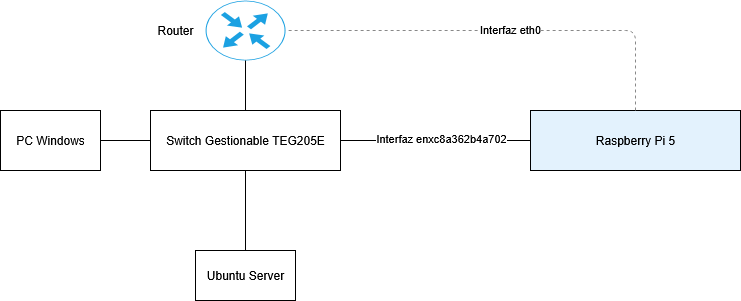
\includegraphics[scale=0.4]{script_automatico/network.png}
	\caption{Esquema de red utilizado en la instalación.}
\end{figure}

\subsection{Hardware (Raspberry Pi 5)}

La \textbf{Raspberry Pi 5} se utiliza como base para la implementación del \textit{NIDS} debido a su bajo consumo energético y su potencia suficiente para analizar tráfico de red en pequeños entornos. Sus características principales incluyen:

\begin{itemize}
	\item \textbf{CPU}: ARM Cortex-A76 (4 núcleos a 2.4 GHz)
	\item \textbf{GPU}: VideoCore VII
	\item \textbf{RAM}: Modelos de 8\,GB LPDDR4X
	\item \textbf{Conectividad}:
	\begin{itemize}
		\item 2 puertos USB 3.0
		\item 2 puertos USB 2.0
		\item 1 puerto Ethernet Gigabit
		\item WiFi 802.11ac y Bluetooth 5.0 (\textit{deshabilitados por seguridad})
	\end{itemize}
	\item \textbf{Almacenamiento}:
	\begin{itemize}
		\item MicroSD de 32\,GB
		\item Soporte para SSD a través de USB 3.0
	\end{itemize}
\end{itemize}

\subsection{Software (Snort y sus complementos)}
\textbf{Snort 3} es un sistema de prevención y detección de intrusos en la red (\textit{NIDS/NIPS}) que introduce una serie de mejoras significativas sobre sus versiones anteriores, incluyendo mayor eficiencia, modularidad y una arquitectura basada en plugins. Estas mejoras hacen que \textbf{Snort 3} sea más \textit{adaptable, eficiente y personalizable} \cite{snort3_vs_snort2}.

\subsubsection{Comparación con Snort 2}
Snort 3 introduce una serie de mejoras sobre Snort 2:
\begin{itemize}
	\item Configuración más flexible y simplificada.
	\item Mayor rendimiento gracias al uso de múltiples hilos.
	\item Soporte para más de 200 plugins que permiten ampliar su funcionalidad.
	\item Sistema de reglas más eficiente y simplificado.
	\item Mejora en la detección de amenazas emergentes y reducción de falsos positivos.
\end{itemize}

\subsubsection{Plugins y complementos utilizados}
Para potenciar las capacidades de detección de \textbf{Snort 3} en este proyecto, se han seleccionado los siguientes \textit{preprocesadores} y herramientas adicionales:

\begin{itemize}
	\item \textbf{HTTP Inspect:} analiza tráfico HTTP/HTTPS para detectar ataques \textit{SQL/XSS} e irregularidades en los encabezados.
	\item \textbf{SSL/TLS:} inspecciona metadatos del tráfico cifrado y detecta conexiones sospechosas o anómalas.
	\item \textbf{Stream IP:} ensambla paquetes IP fragmentados para detectar intentos de evasión.
	\item \textbf{Stream TCP:} reensambla flujos TCP/UDP para un análisis más preciso.
	\item \textbf{Reputation Preprocessor:} bloquea tráfico de fuentes maliciosas basado en listas de reputación. 
	\item \textbf{Conjunto de reglas de datos sensibles:} detecta información sensible como números de tarjetas de crédito o credenciales expuestas.
	\item \textbf{ClamAV:} sistema antivirus de código abierto que complementa la detección de amenazas de Snort con análisis basado en firmas.
\end{itemize}


\newpage

\section{Instalación y personalización de complementos}
\subsection{Instalación de Snort V3}
% Contenido de la sección 2.4
El desarrollo de lo que será \textbf{R-SNORT} empezará con la instalación de \textbf{Snort} \cite{snort3_installation_pdf} mismo en su versión actual. Para ello, es buena práctica actualizar los repositorios y el equipo mediante un \texttt{update} y un \texttt{upgrade} antes de comenzar la instalación. Una vez hecho esto, empezaremos con la instalación de las distintas librerías y dependencias de \textbf{Snort V3}.
\newline

Primero, instalamos un par de herramientas necesarias (\texttt{libtool} y \texttt{autoconf}) para compilar Snort 3. Luego, nos movemos al directorio \texttt{/usr/local/src} y clonamos el repositorio de \texttt{libdnet} desde GitHub, que es una librería importante para que Snort funcione correctamente. Finalmente, entramos en el directorio \texttt{libdnet} para seguir con la instalación.

\begin{figure}[H]
	\centering
	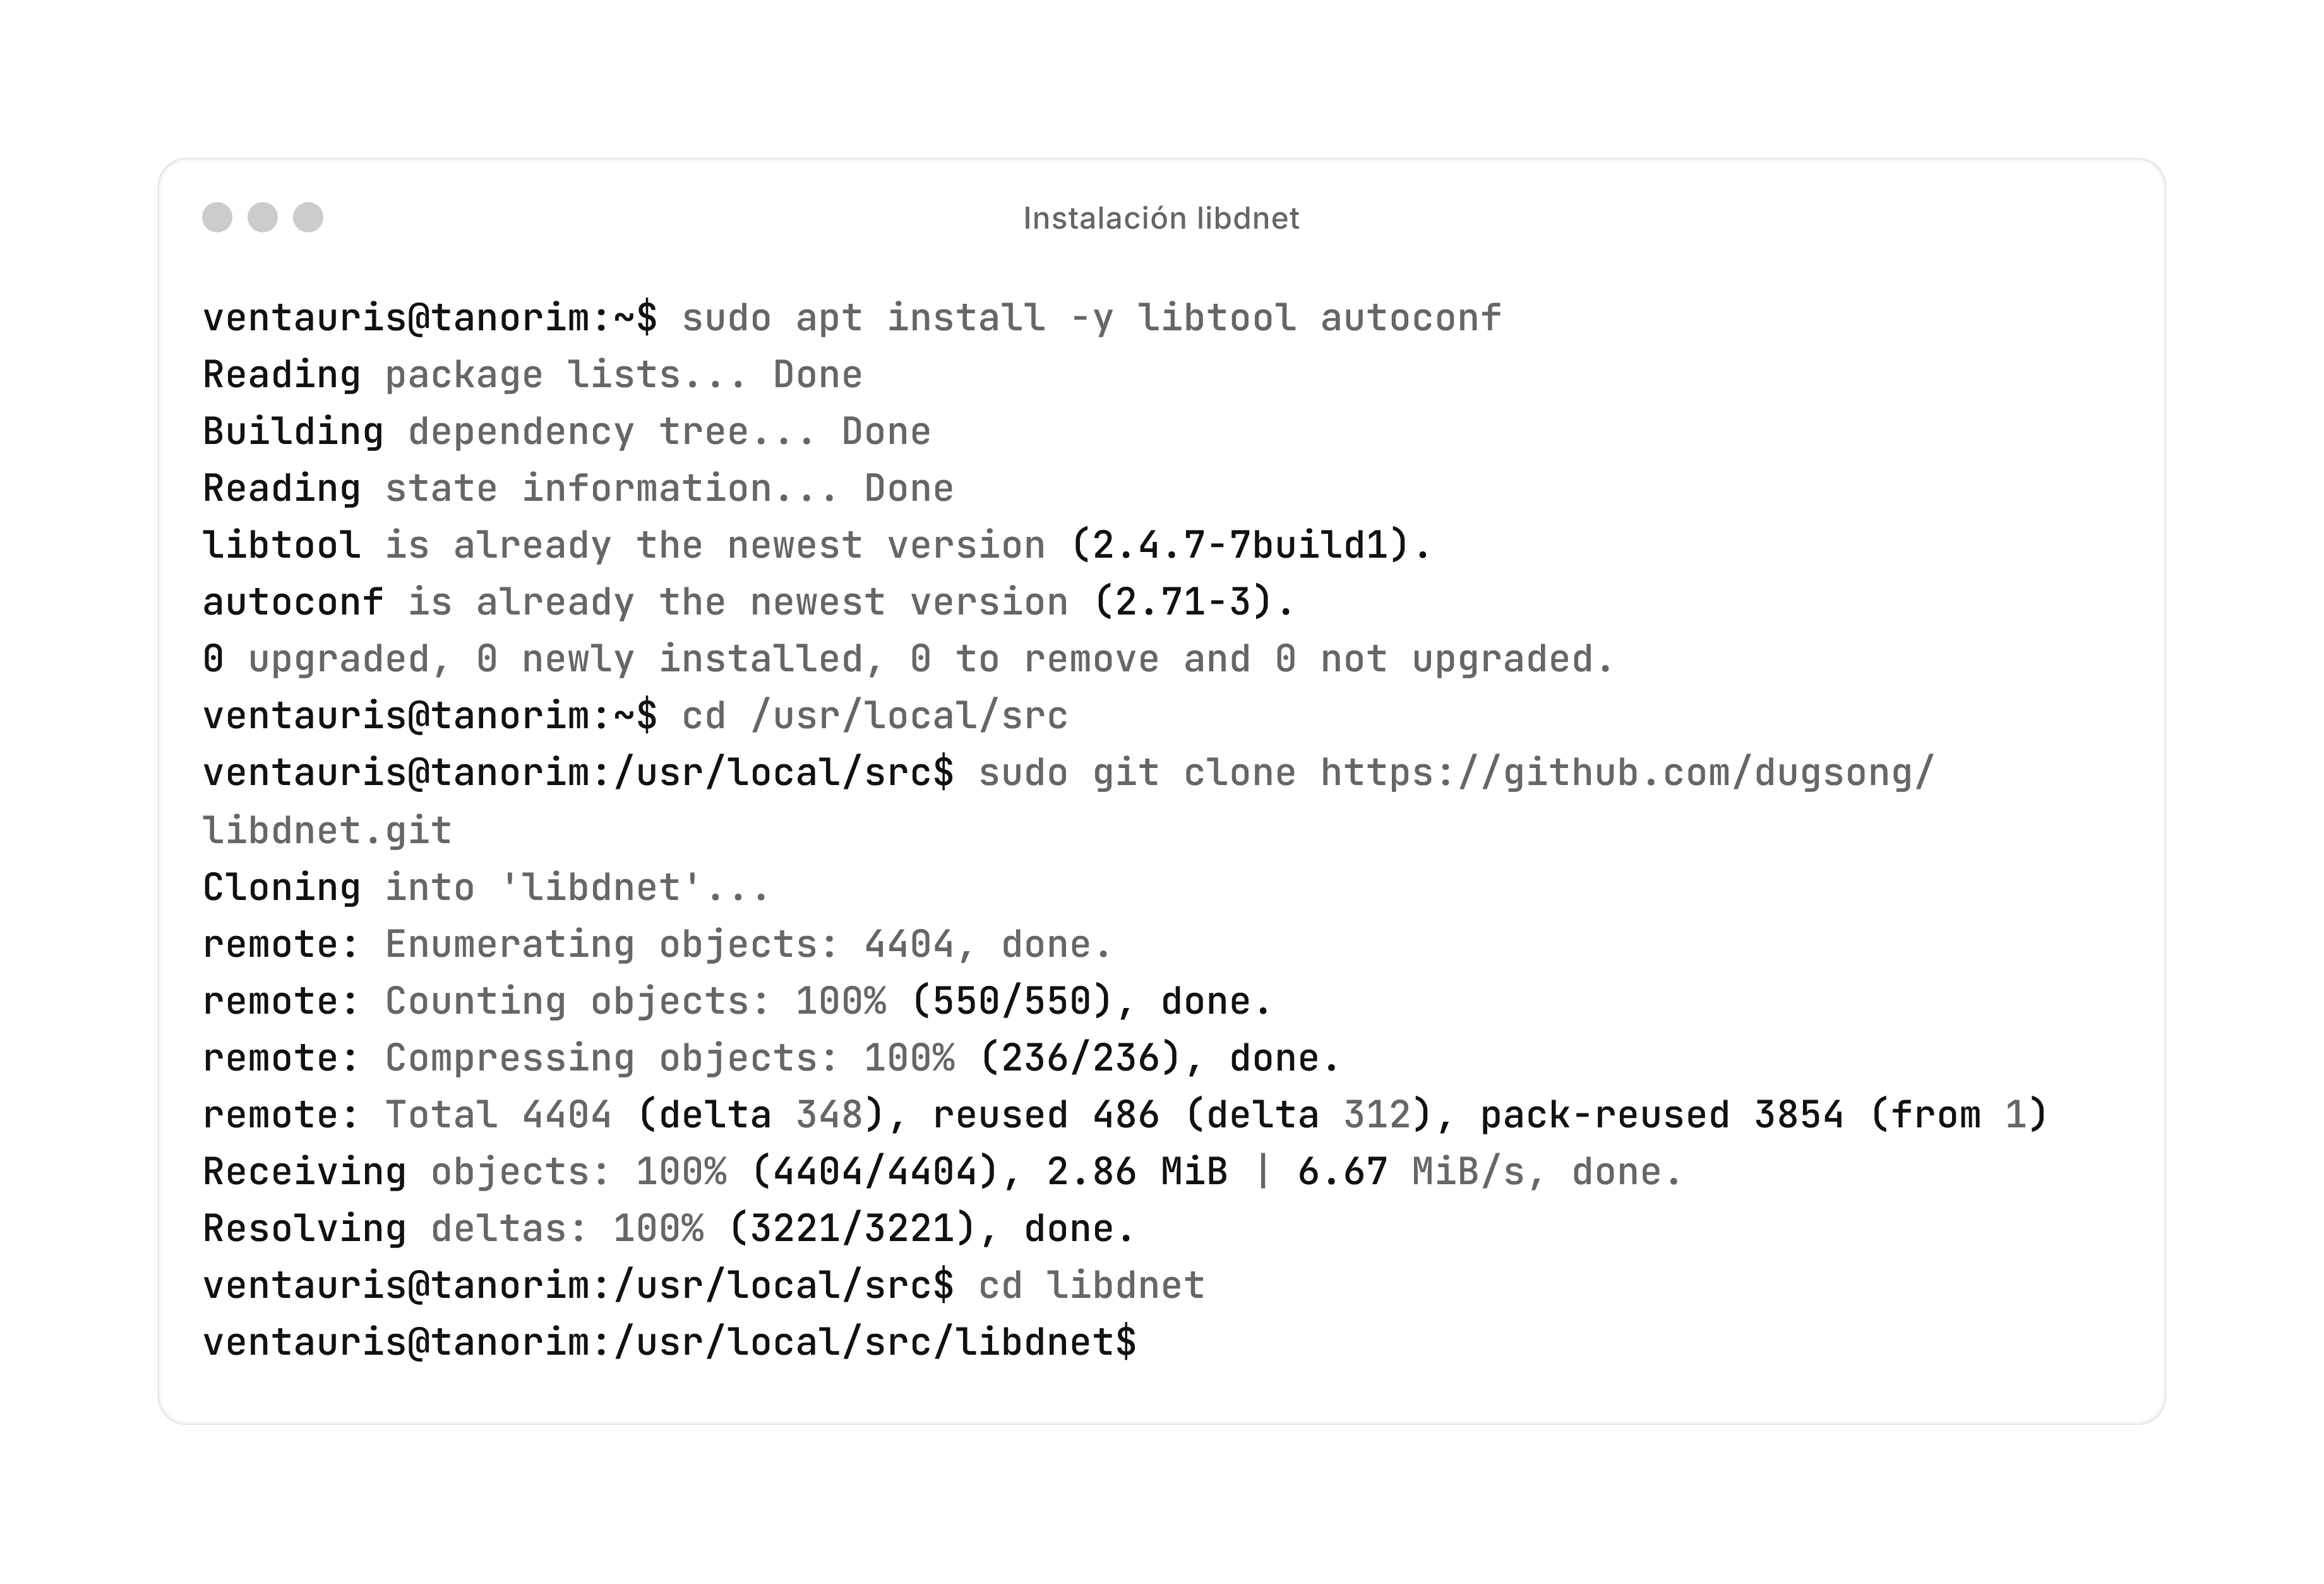
\includegraphics[scale=0.12]{instalacion_snort/1-1.png}
	\caption{Instalando dependencias necesarias.}
\end{figure}

\newpage

A continuación, el paquete \texttt{check} es instalado. Esta herramienta servirá principalmente para ejecutar algunas pruebas en C. Es un requisito para poder compilar \texttt{libdnet} correctamente. Gracias a estas preparaciones, estamos configurando el entorno para la correcta compilación de Snort.

\begin{figure}[H]
	\centering
	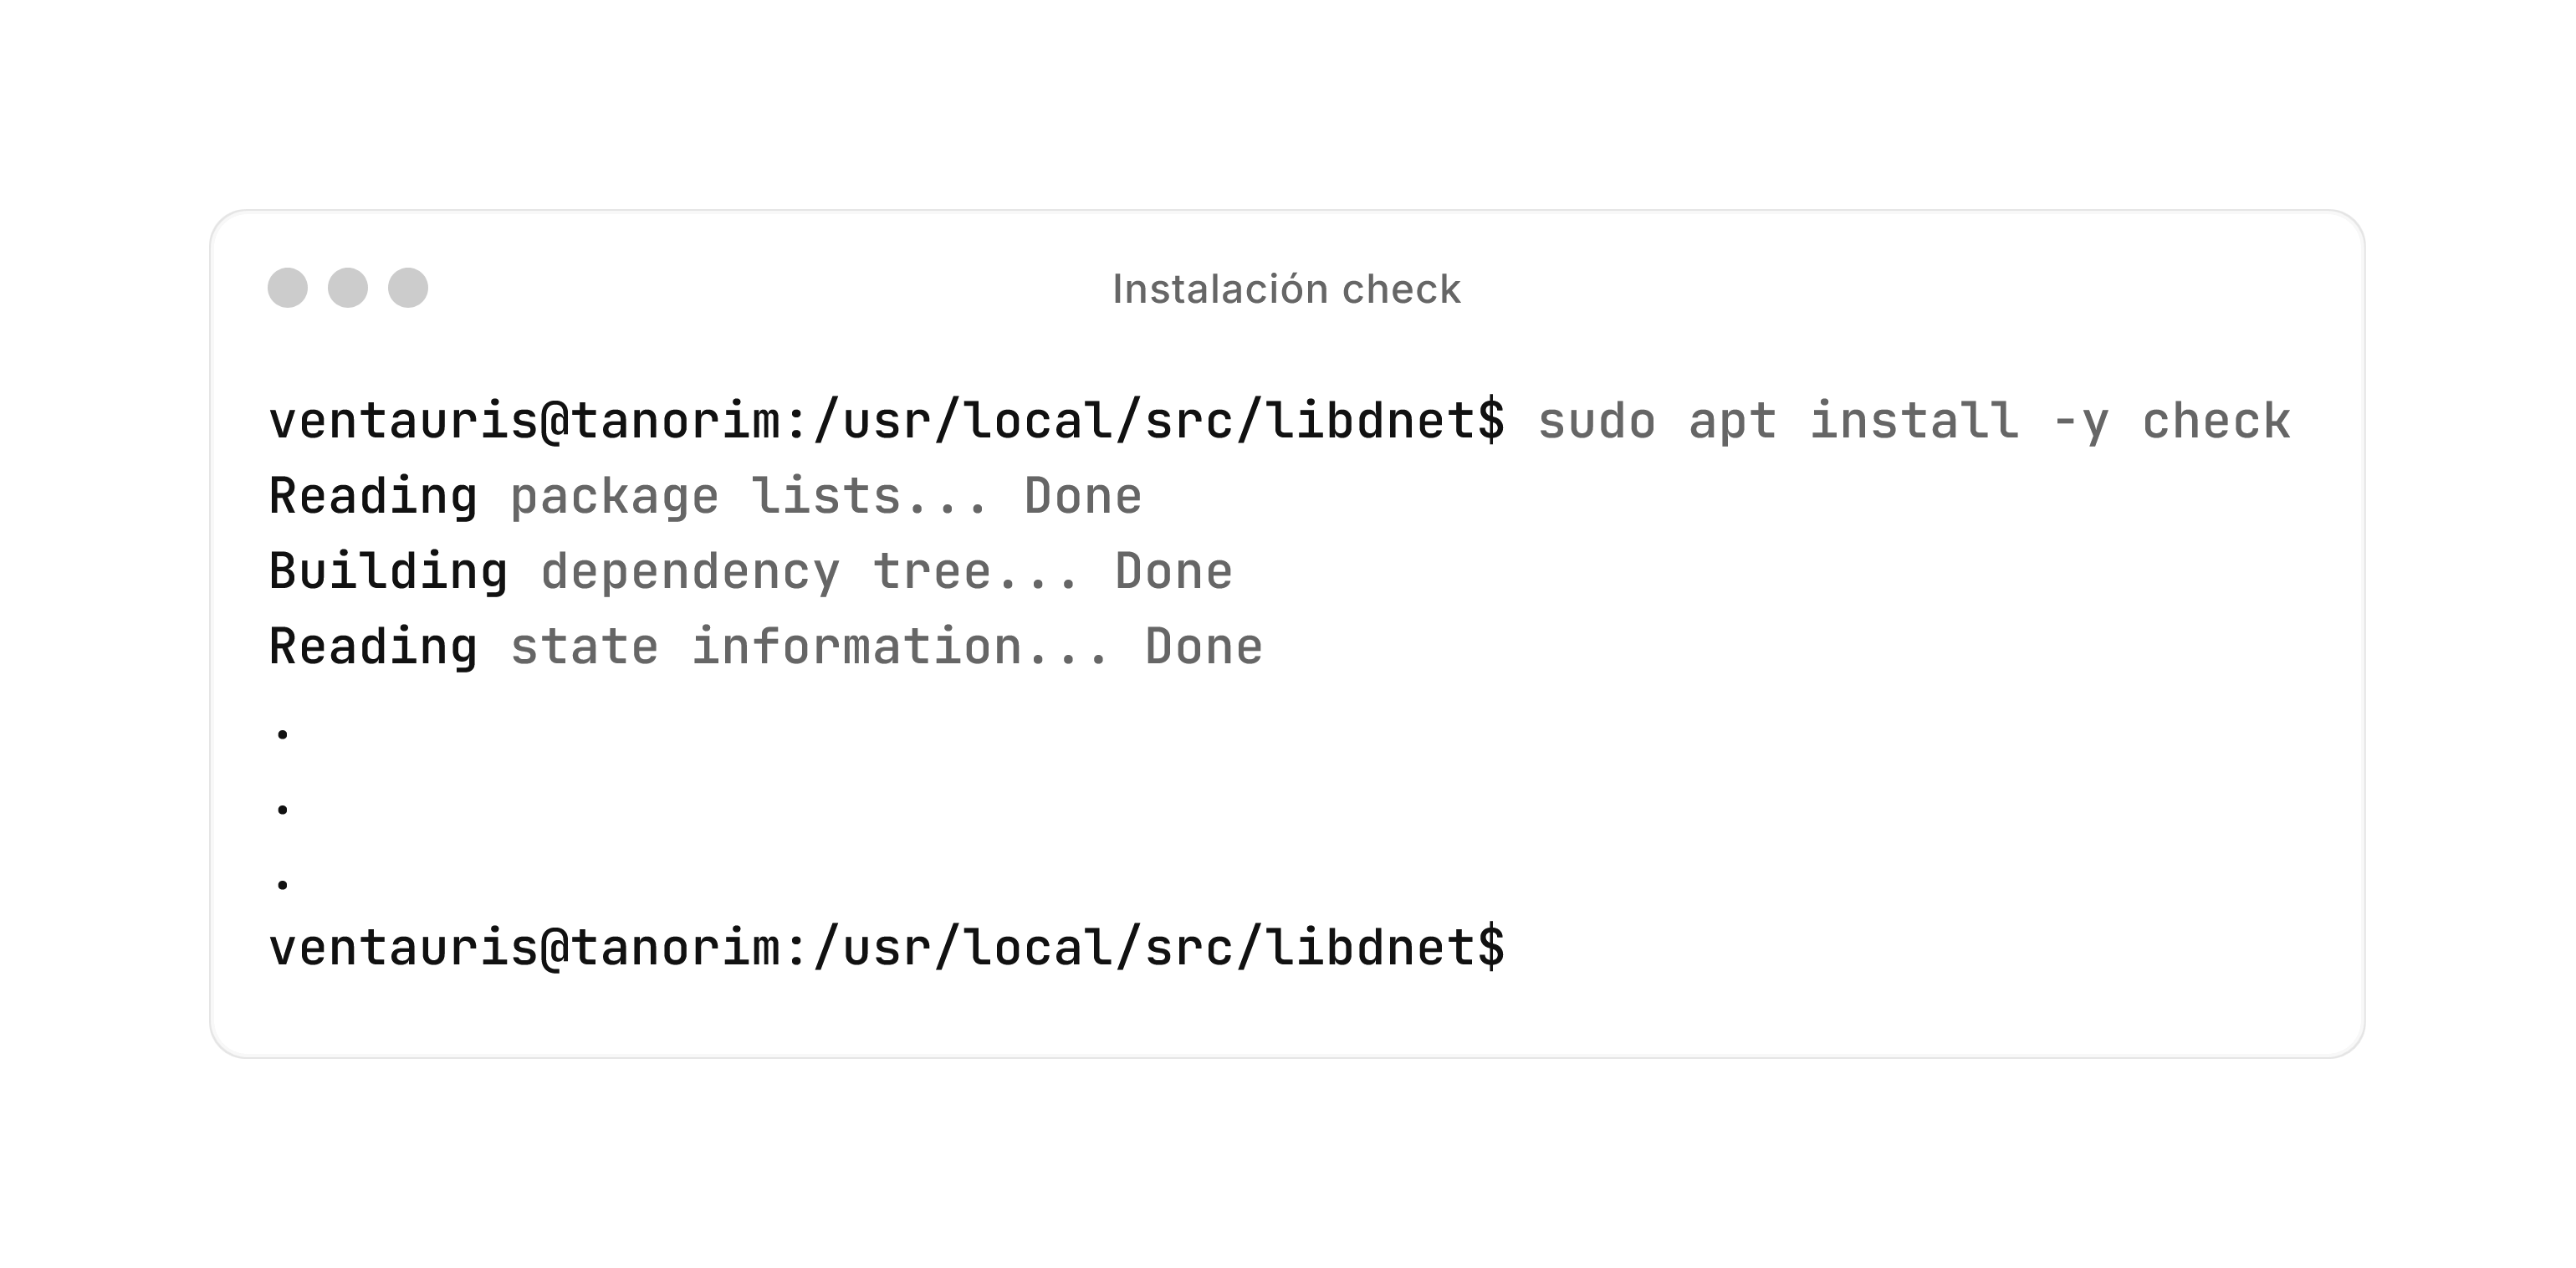
\includegraphics[scale=0.12]{instalacion_snort/2-2.png}
	\caption{Instalando dependencia \texttt{check}.}
\end{figure}

La ejecución de \texttt{./configure} prepara el entorno para la compilación de \texttt{libdnet}, dependencia fundamental para el correcto funcionamiento del desarrollo posterior y de Snort. Su funcionamiento consiste en la revisión del sistema, verifica dependencias y configura los archivos necesarios para compilar código correctamente.

\begin{figure}[H]
	\centering
	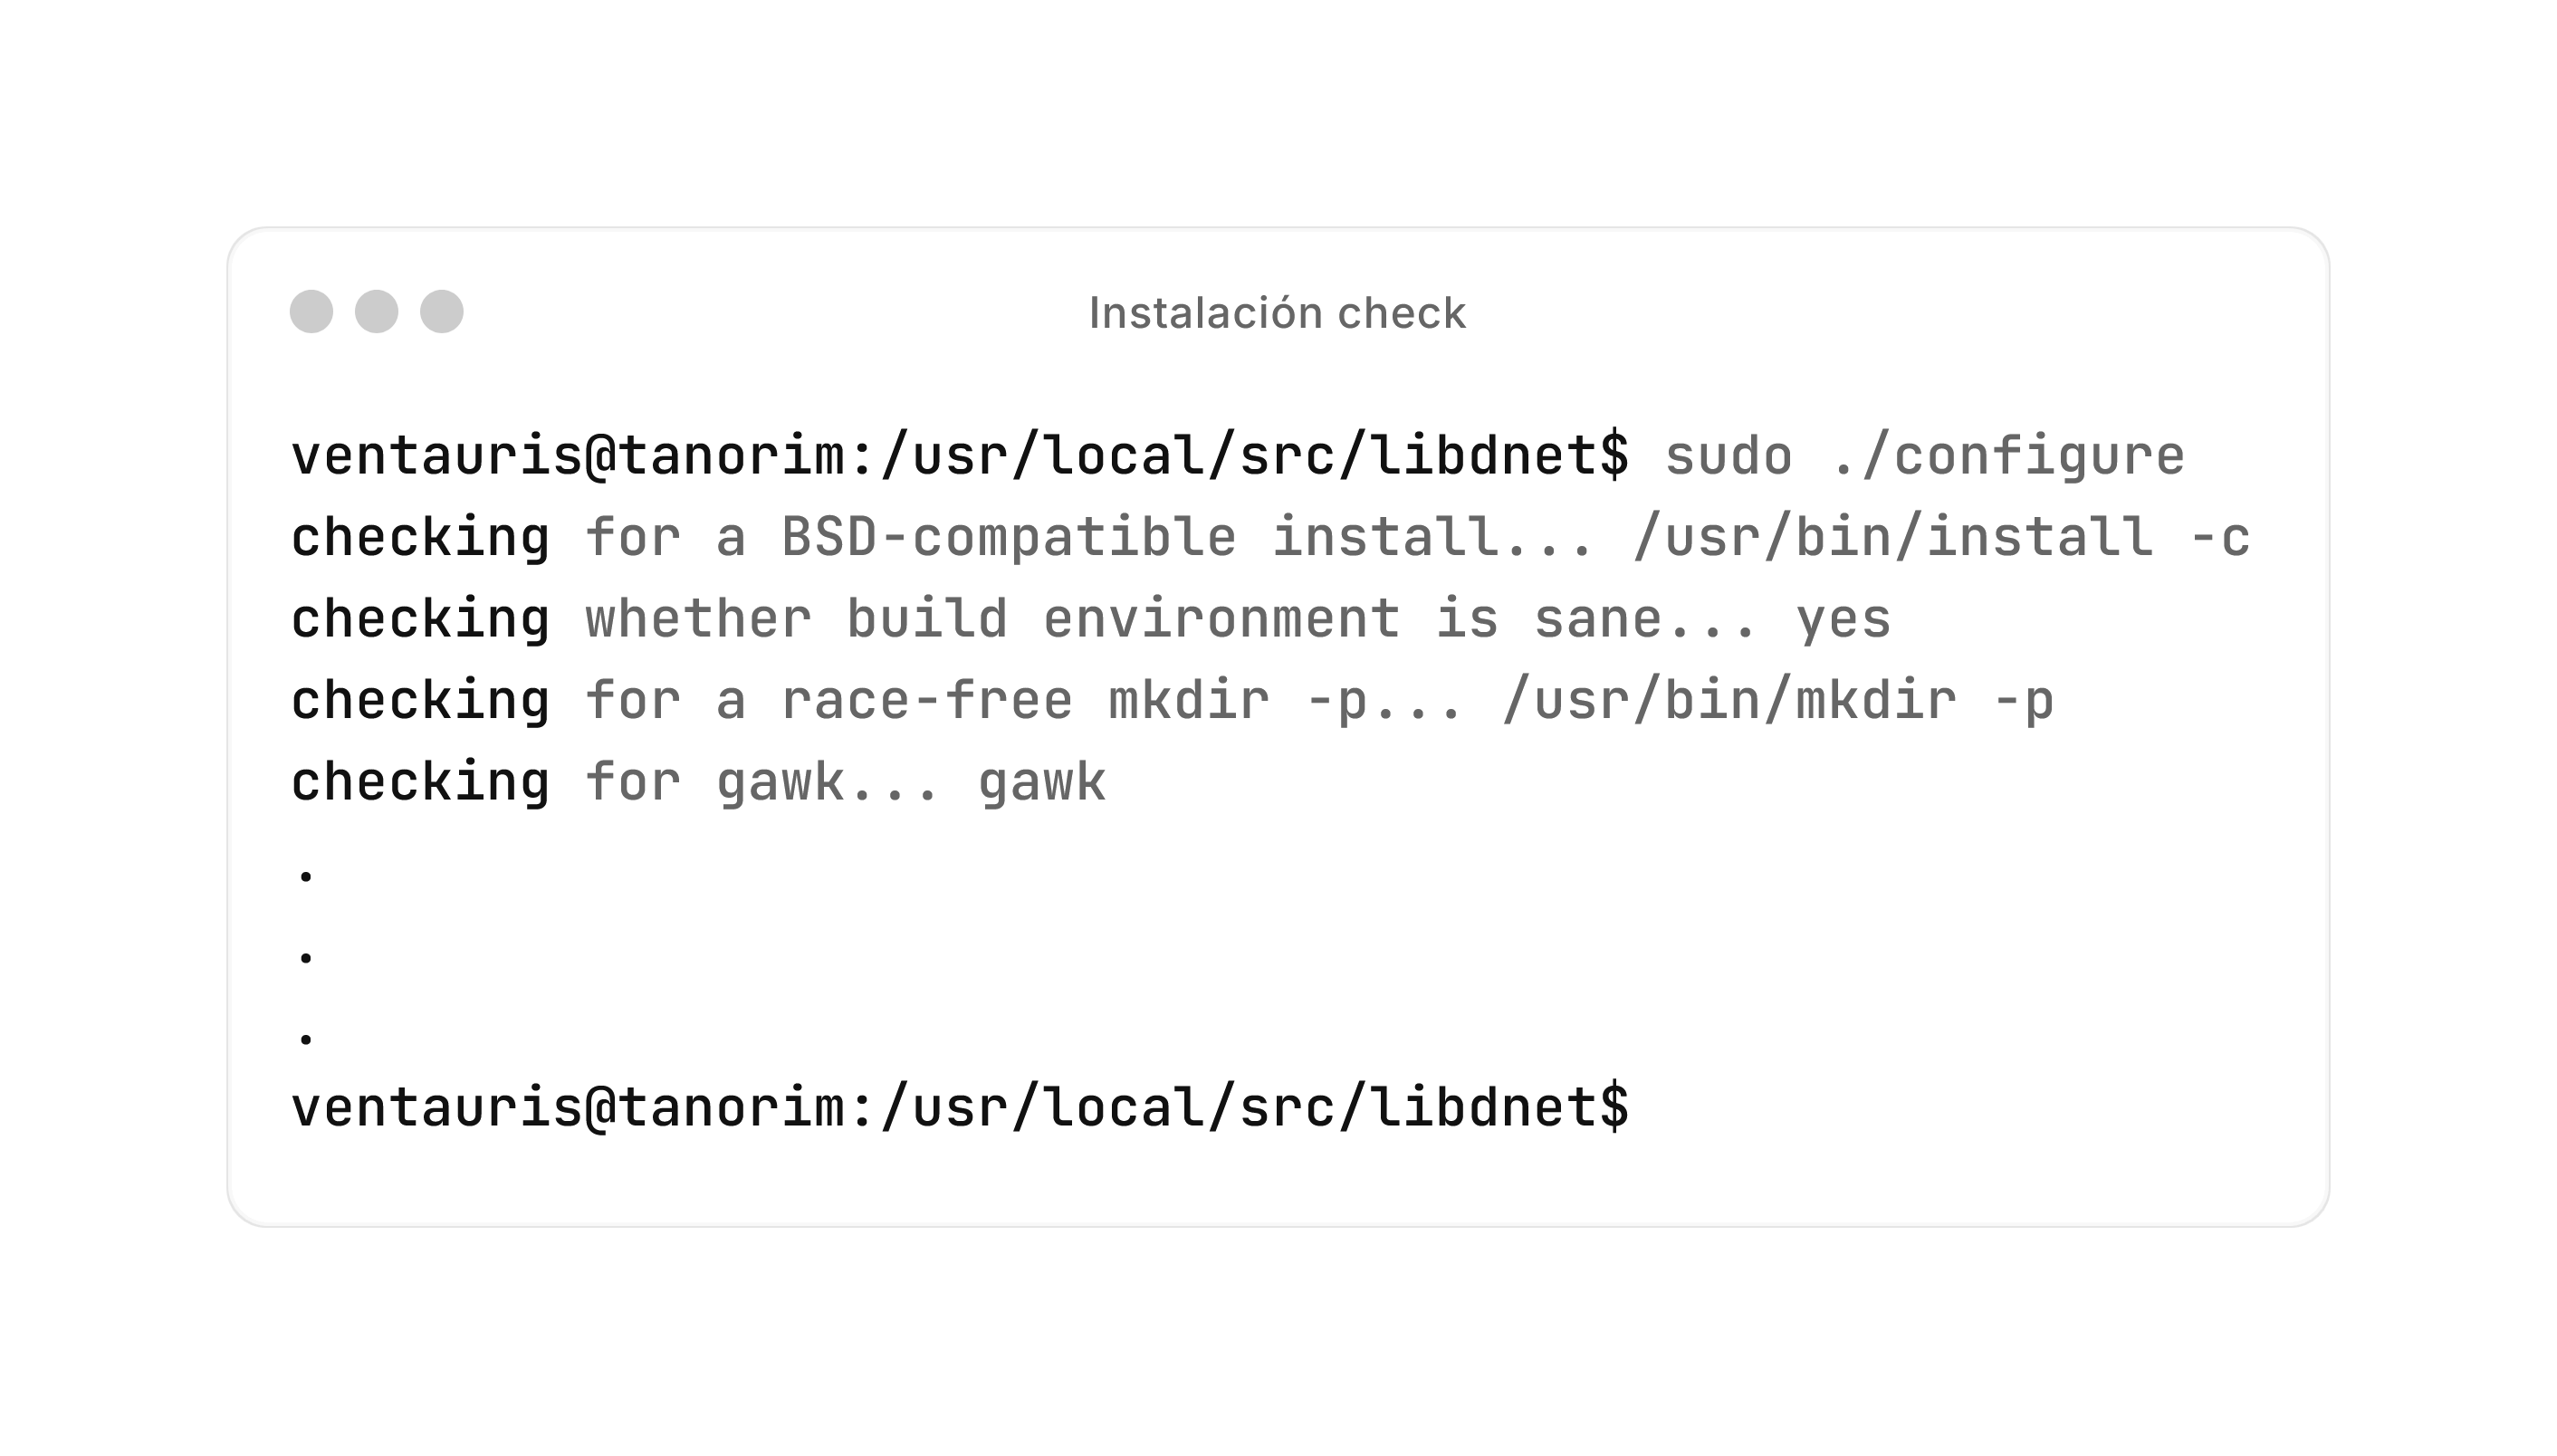
\includegraphics[scale=0.12]{instalacion_snort/3-3.png}
	\caption{Configurando \texttt{libdnet} antes de la compilación.}
\end{figure}

\newpage

Llevamos a cabo la compilación de \texttt{libdnet} mediante \texttt{sudo make}; este comando convierte el código fuente de la dependencia en un ejecutable con bibliotecas a disposición para la instalación. Recorre los directorios del proyecto asegurándose de que todos los archivos necesarios sean procesados.

\begin{figure}[H]
	\centering
	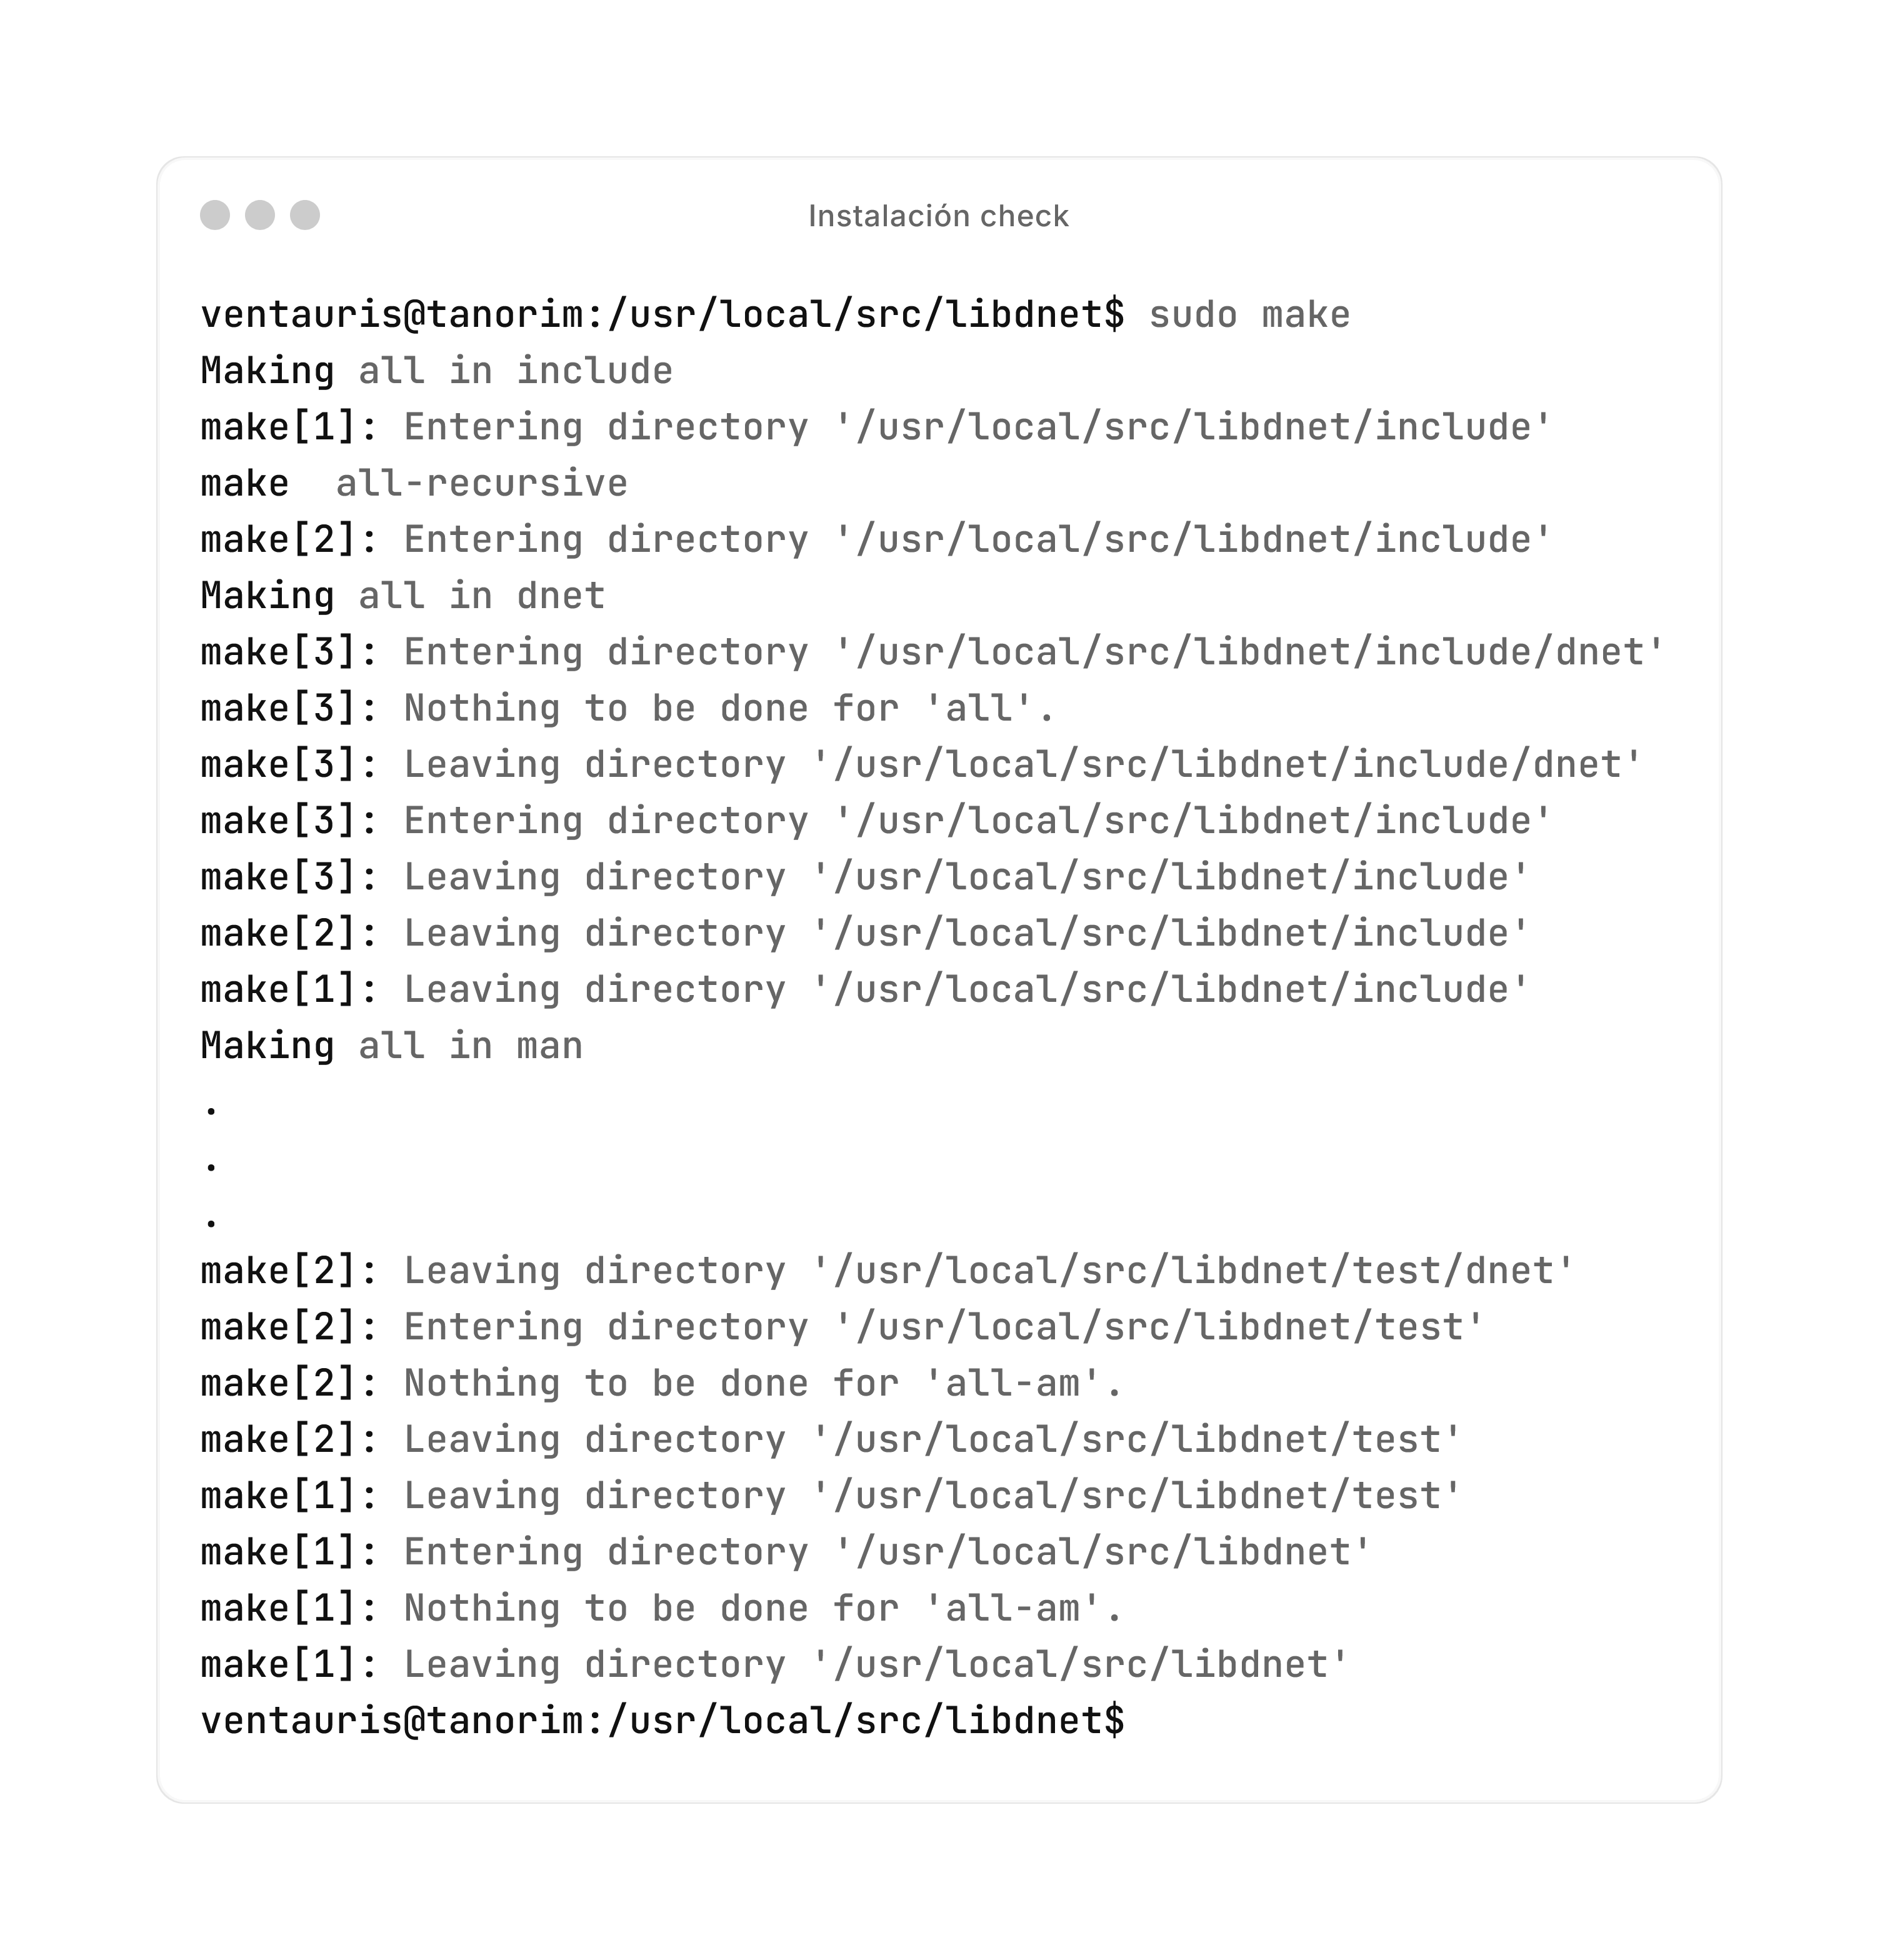
\includegraphics[scale=0.12]{instalacion_snort/4-4.png}
	\caption{Compilando \texttt{libdnet} con \texttt{make}.}
\end{figure}


\newpage

Ahora usamos \texttt{sudo make install} para instalar \texttt{libdnet} en el sistema. Este comando copia los archivos compilados a sus directorios correspondientes, asegurando que puedan ser utilizados por otras aplicaciones y librerías.

\begin{figure}[H]
	\centering
	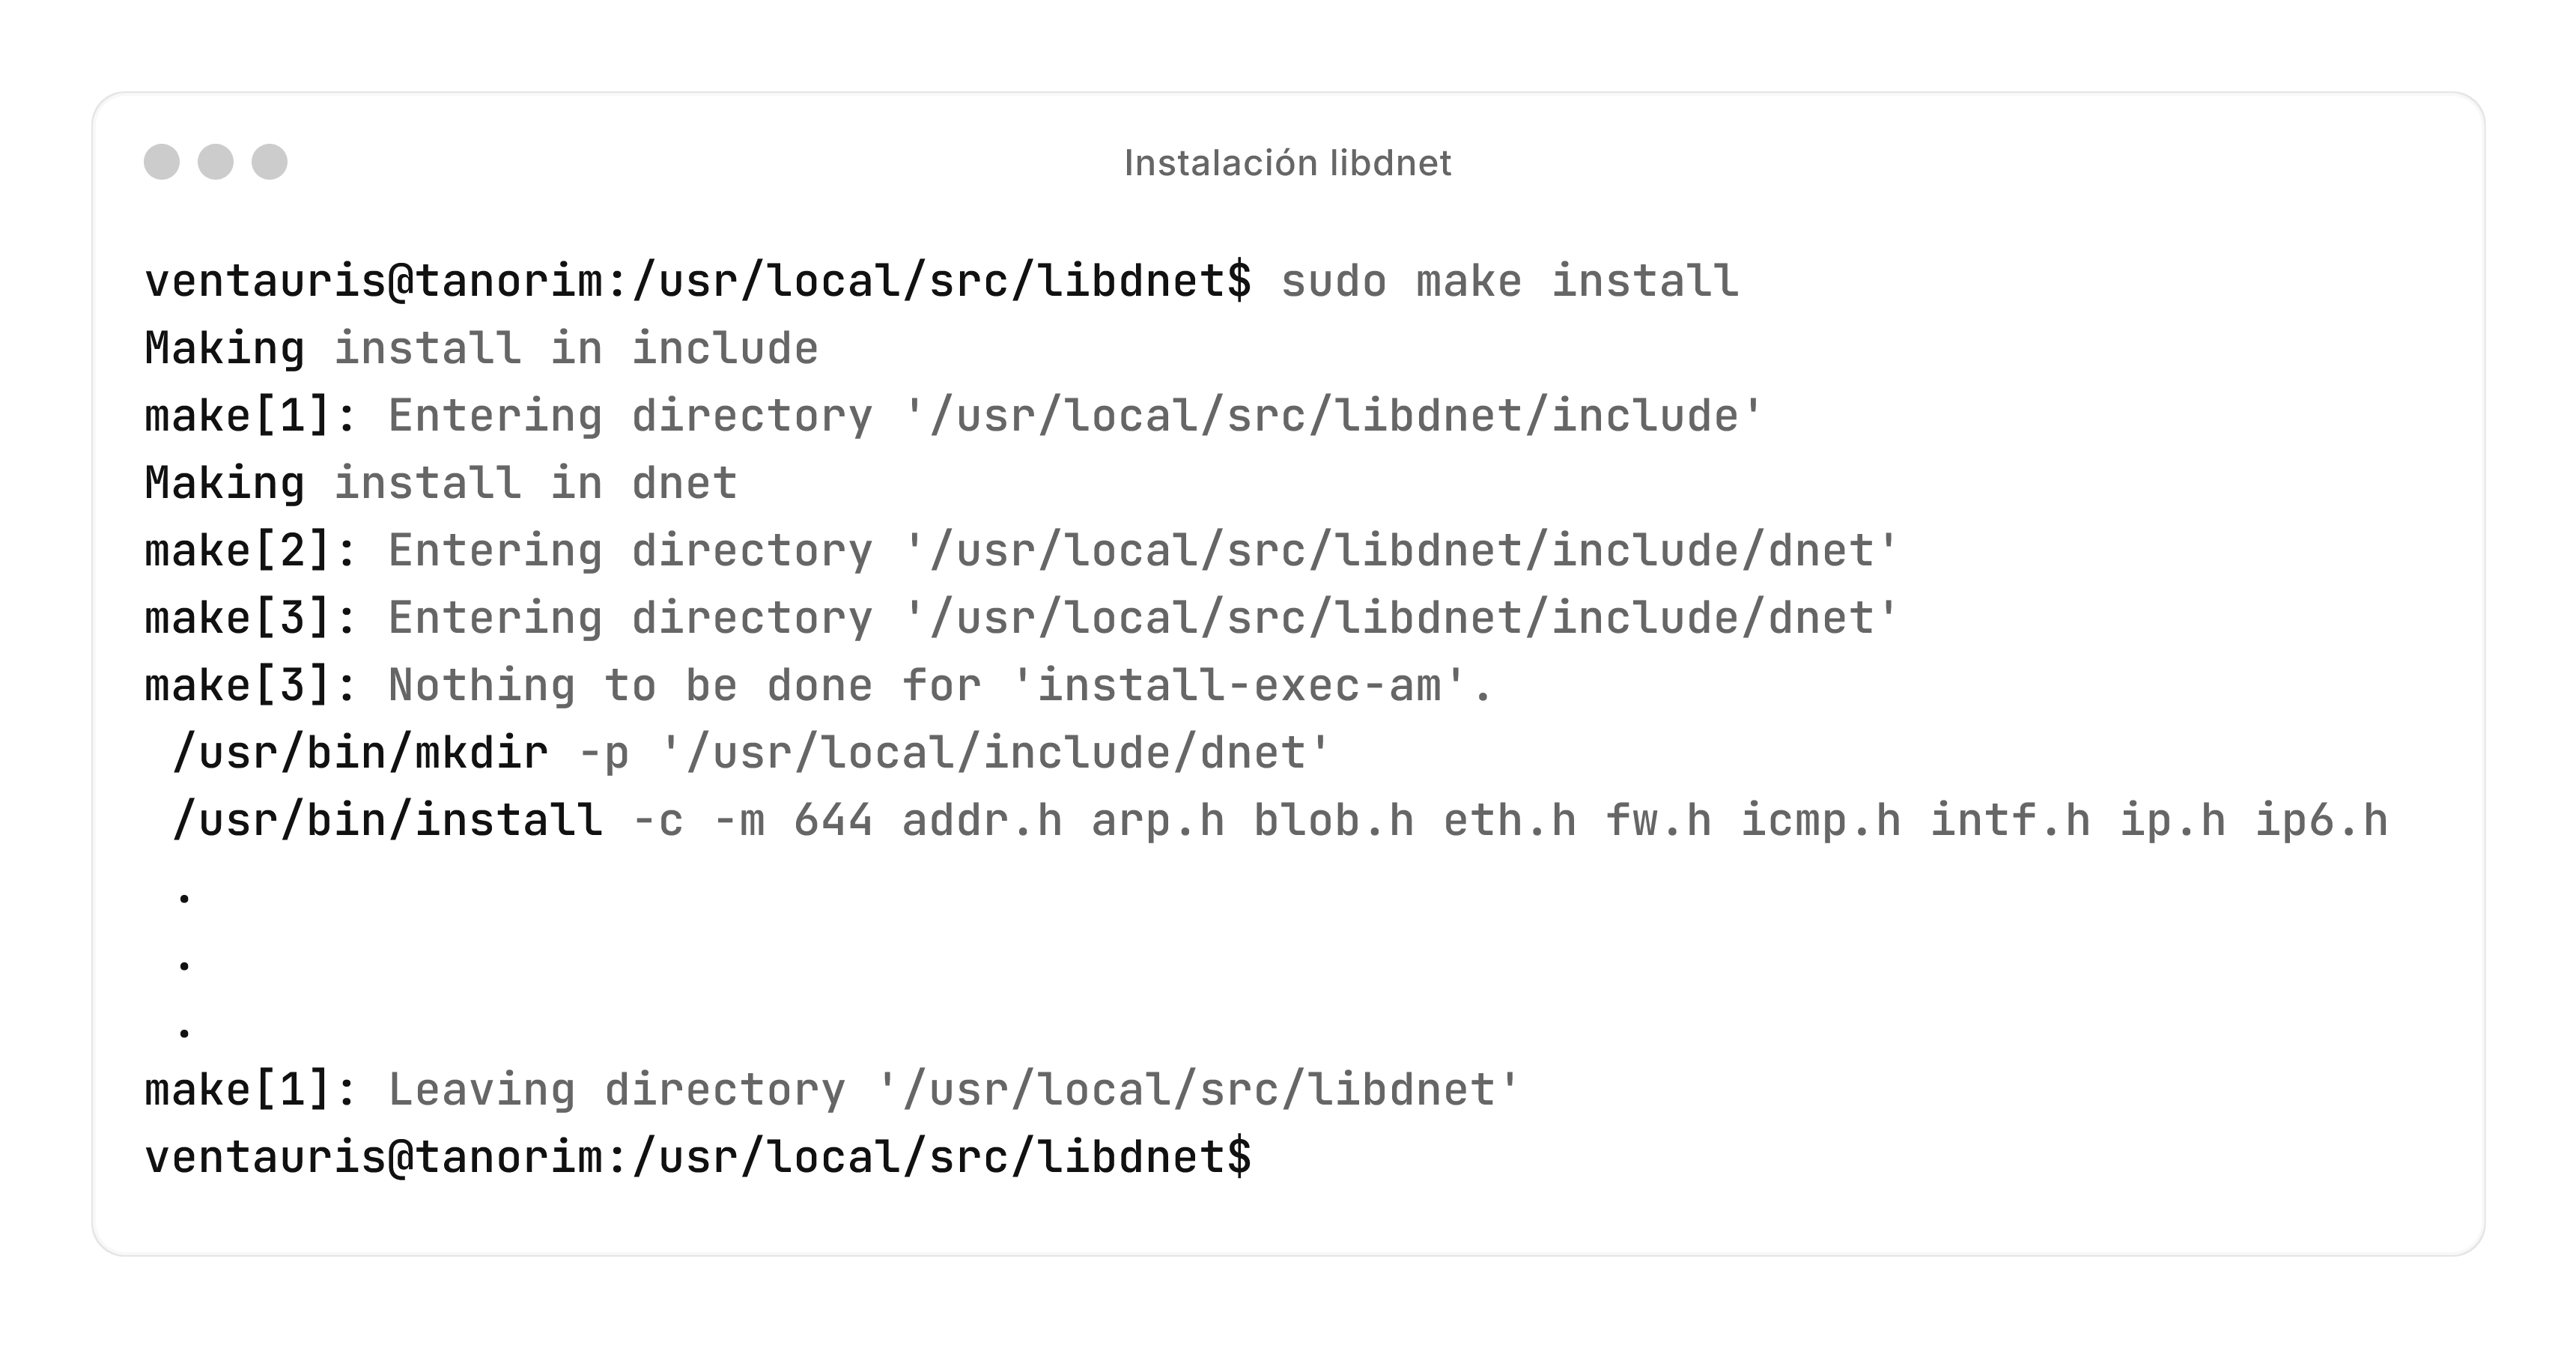
\includegraphics[scale=0.12]{instalacion_snort/5-5.png}
	\caption{Instalando \texttt{libdnet} en el sistema.}
\end{figure}

Listamos los archivos de \texttt{libdnet} en \texttt{/usr/local/lib} para asegurarnos de que se instalaron correctamente. Luego, intentamos verificar su versión con \texttt{pkg-config --modversion dnet}, pero aparece un error indicando que no se encuentra en el \texttt{PKG\_CONFIG\_PATH}. Esto indica que es necesario añadir la ruta correcta para que el sistema reconozca la librería.

\begin{figure}[H]
	\centering
	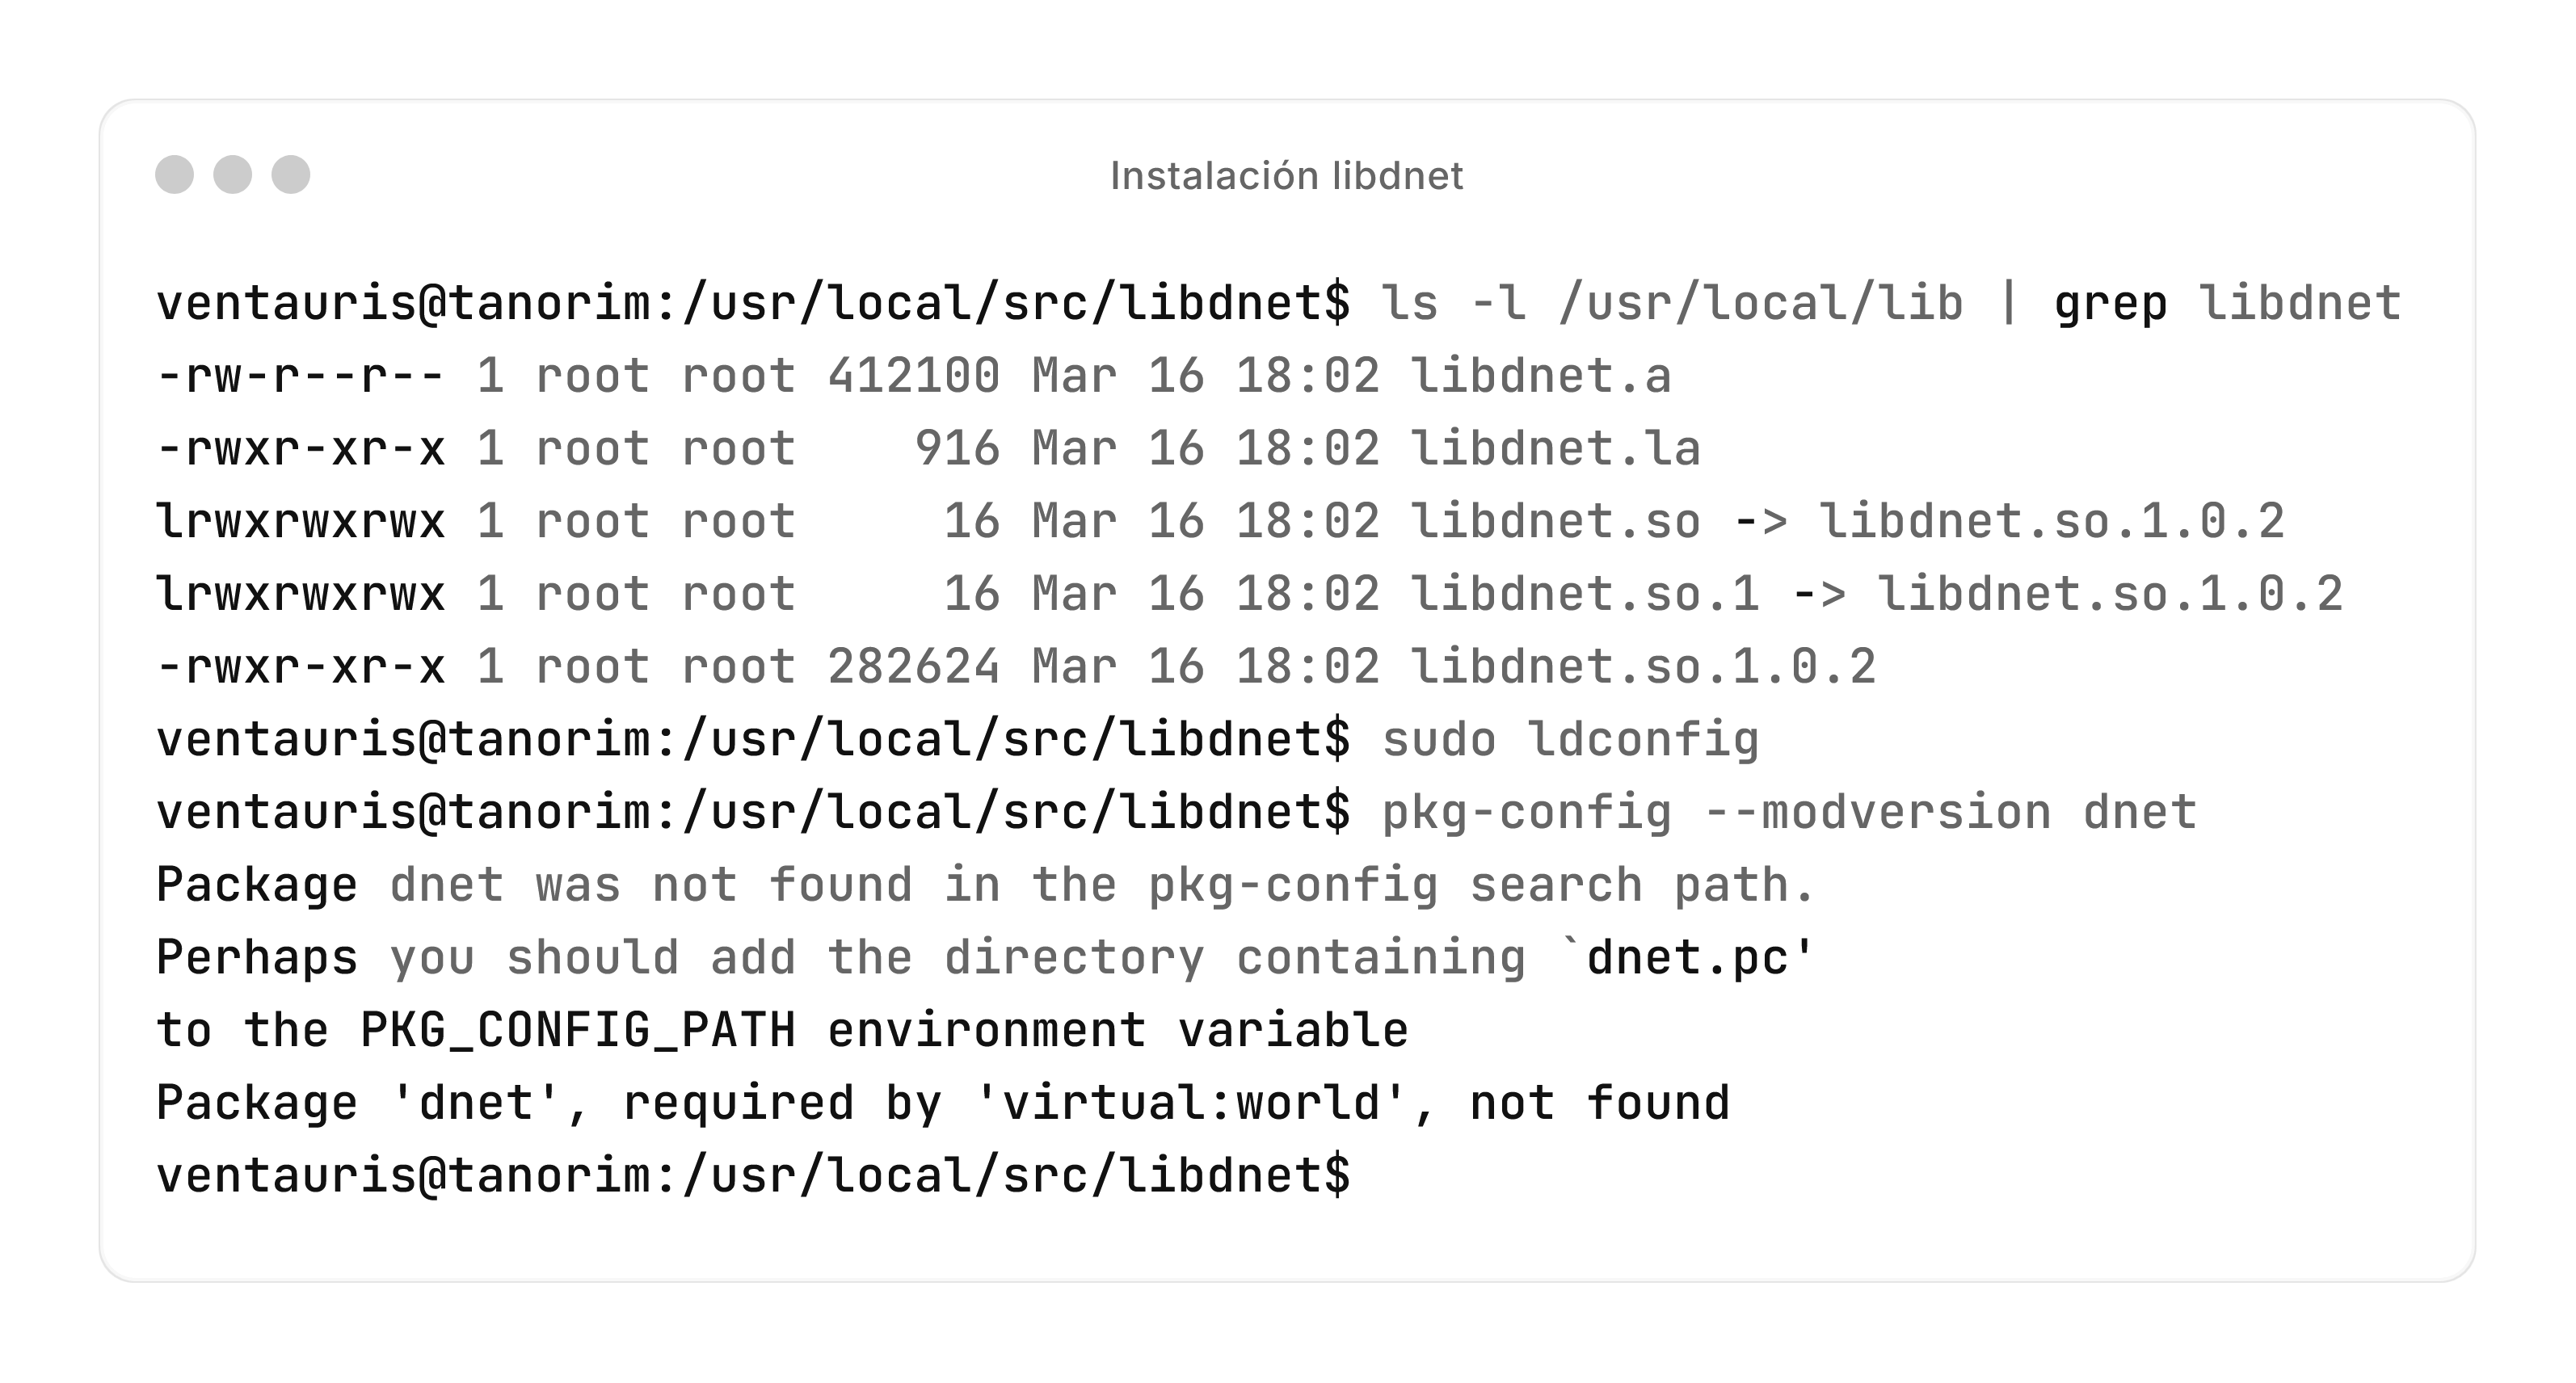
\includegraphics[scale=0.12]{instalacion_snort/6-6.png}
	\caption{Verificación de la instalación de \texttt{libdnet}.}
\end{figure}

\newpage

Hemos editado el archivo \texttt{dnet.pc} usando \texttt{nano}, añadiendo las rutas correctas para que \texttt{pkg-config} pueda encontrar \texttt{libdnet}. Definimos las variables \texttt{libdir} e \texttt{includedir}, asegurándonos de que apunten a \texttt{/usr/local/lib} y \texttt{/usr/local/include}, respectivamente. Esto soluciona el problema anterior donde \texttt{pkg-config} no encontraba la librería.

\begin{figure}[H]
	\centering
	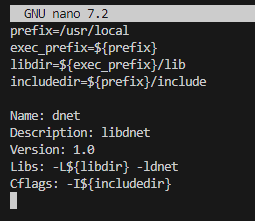
\includegraphics[scale=1]{instalacion_snort/7.png}
	\caption{Configurando \texttt{libdnet} para que sea reconocido por el sistema.}
\end{figure}

Ahora configuramos el entorno para que \texttt{pkg-config} pueda encontrar \texttt{libdnet}. Primero, exportamos la variable \texttt{PKG\_CONFIG\_PATH} con la ruta correcta y la agregamos permanentemente al archivo \texttt{\~{}/.bashrc}. Luego, recargamos la configuración con \texttt{source ~/.bashrc}, actualizamos las librerías con \texttt{ldconfig} y verificamos que \texttt{libdnet} es reconocido correctamente ejecutando \texttt{pkg-config --modversion dnet}, confirmando la versión instalada.

\begin{figure}[H]
	\centering
	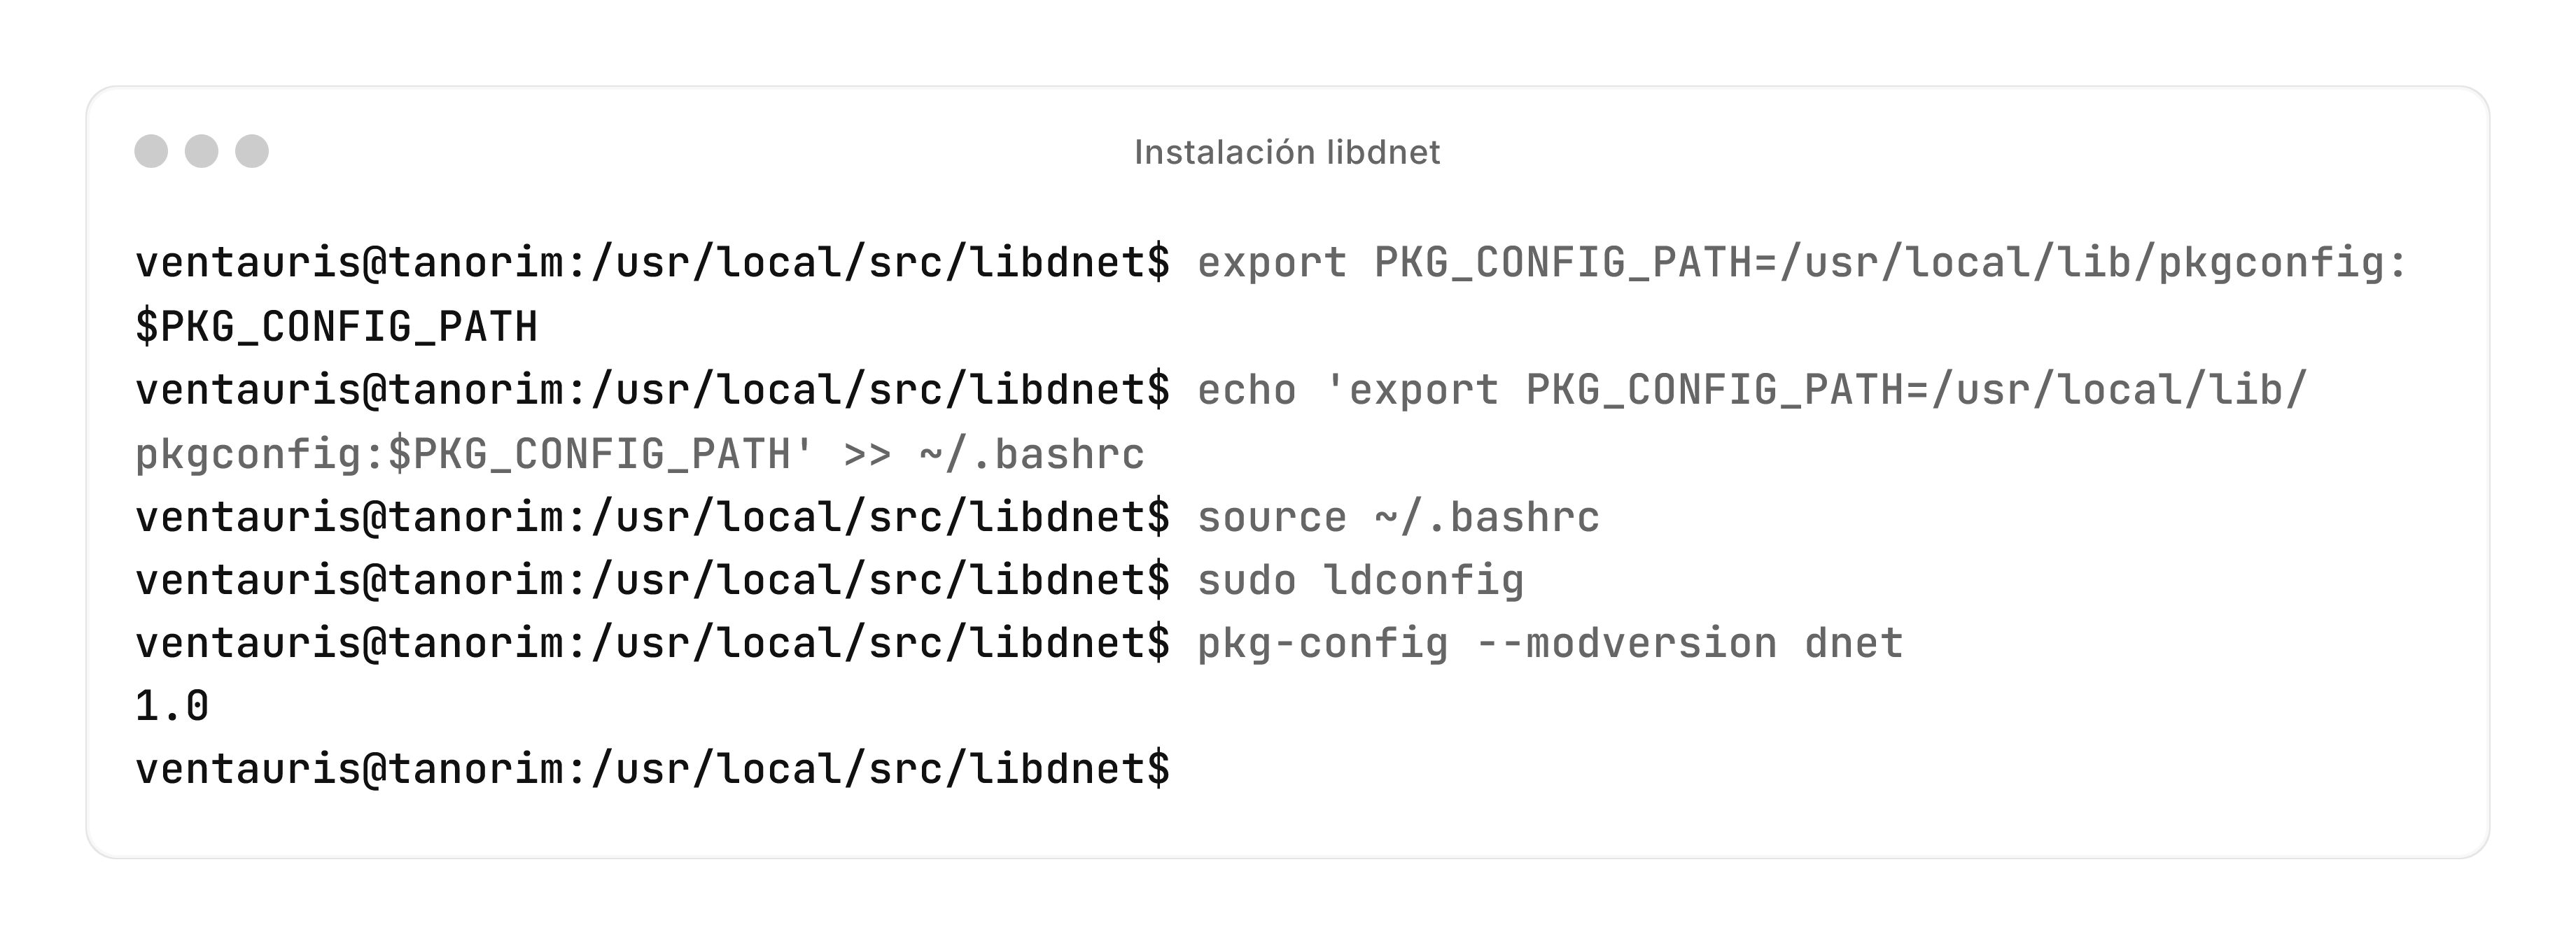
\includegraphics[scale=0.12]{instalacion_snort/8-8.png}
	\caption{Añadiendo \texttt{libdnet} al \texttt{PATH} y verificando su reconocimiento.}
\end{figure}

\newpage

Clonamos el repositorio de \texttt{libdaq}, un componente necesario para \textbf{Snort 3}, desde su fuente oficial en GitHub. Este paso descarga el código fuente necesario para su compilación e instalación en la \textbf{Raspberry Pi}.

\begin{figure}[H]
	\centering
	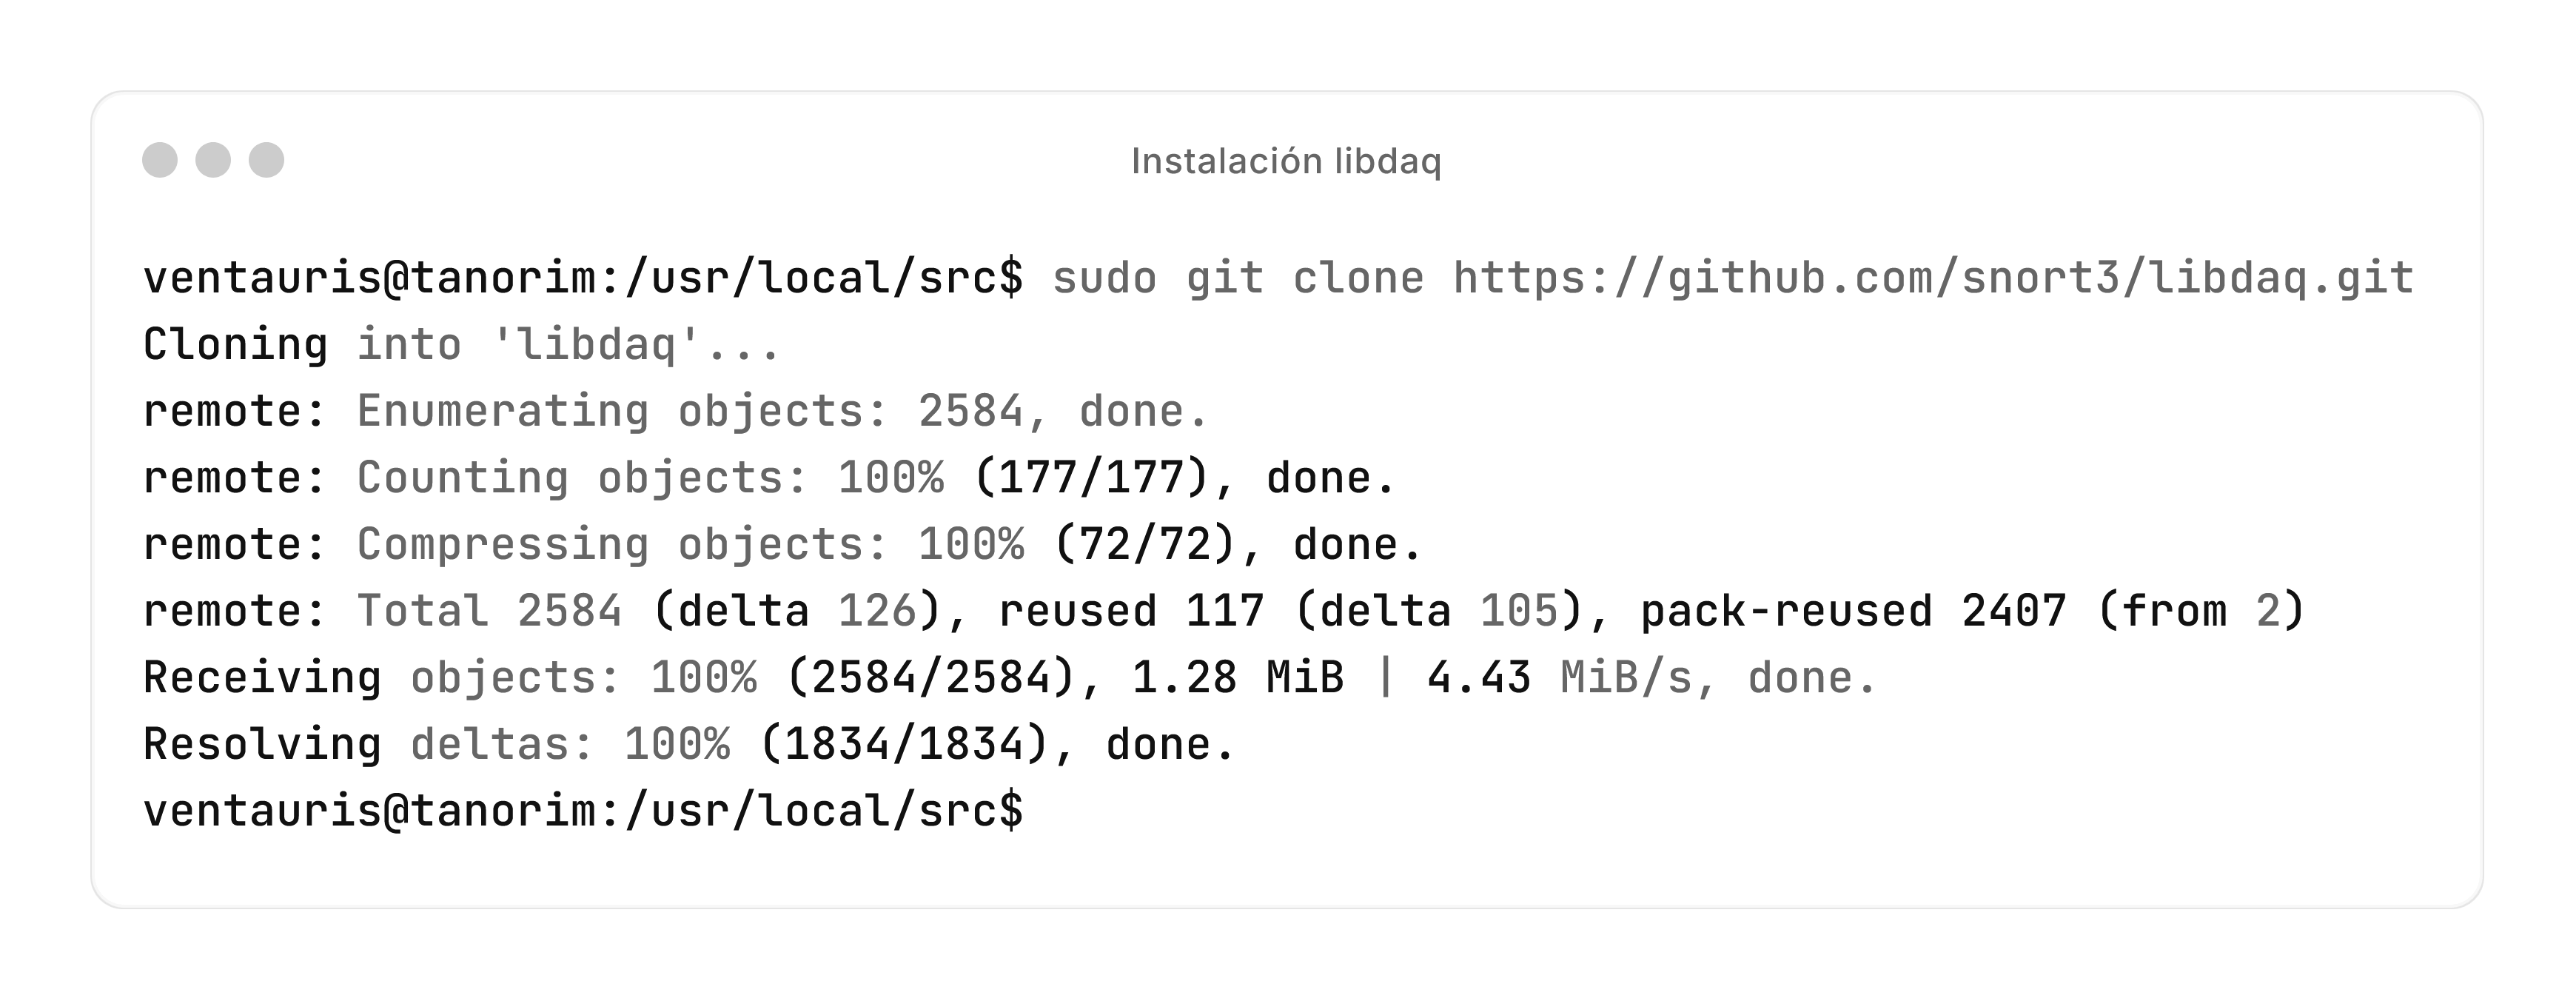
\includegraphics[scale=0.12]{instalacion_snort/9-9.png}
	\caption{Descargando \texttt{libdaq} desde el repositorio oficial.}
\end{figure}

Entramos en el directorio de \texttt{libdaq} y ejecutamos el script \texttt{bootstrap}, que se encarga de generar los archivos de configuración necesarios para compilar el software correctamente. Se usa \texttt{autoreconf} para asegurarse de que todos los scripts de compilación estén en orden.

\begin{figure}[H]
	\centering
	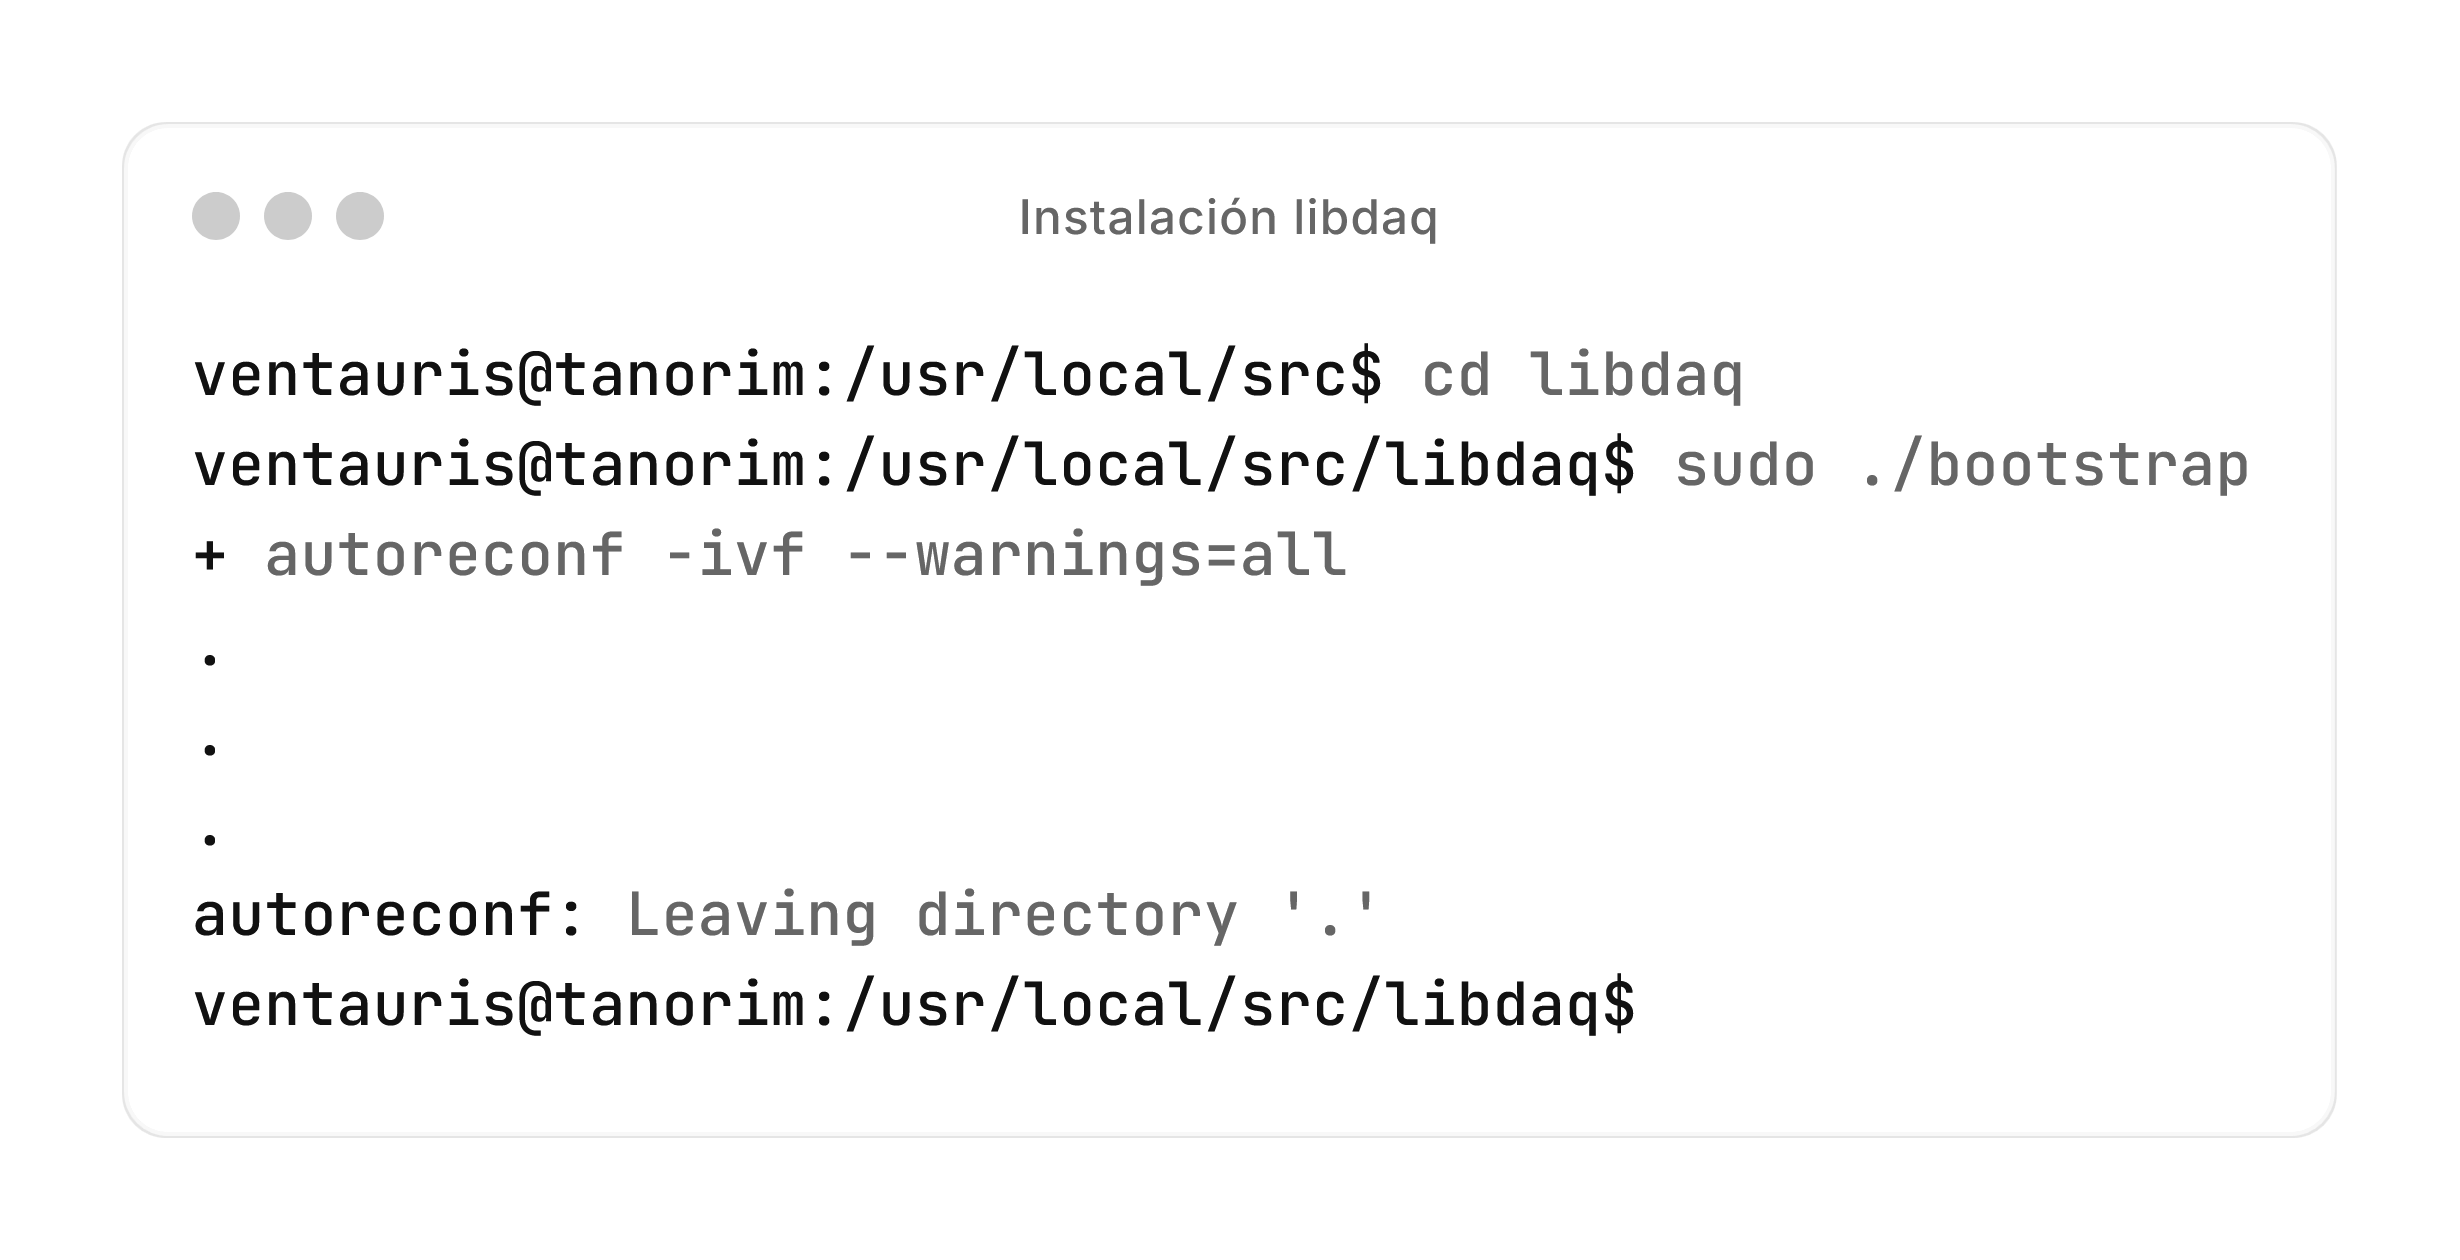
\includegraphics[scale=0.12]{instalacion_snort/10-10.png}
	\caption{Preparando \texttt{libdaq} para su compilación.}
\end{figure}

\newpage

%%%%%%%%%%%%%%%%%%%%%%%%%%%%%%%%%%%%%%%%%%%%%HECHO2%%%%%%%%%%%%%%%%%%%%%%%%%%%%%%%%%%%%%%%%%%%%%%%%%%%%%%%%%%%%%%%%%%%%%%%%%%%%%%%%%%%%%%%%%

Ejecutamos \texttt{./configure} para preparar el entorno de compilación de \texttt{libdaq}. Como se ha comentado anteriormente, este script revisa que el sistema tenga todas las dependencias necesarias y genera los archivos de configuración adecuados para compilar el software sin complicaciones.

\begin{figure}[H]
	\centering
	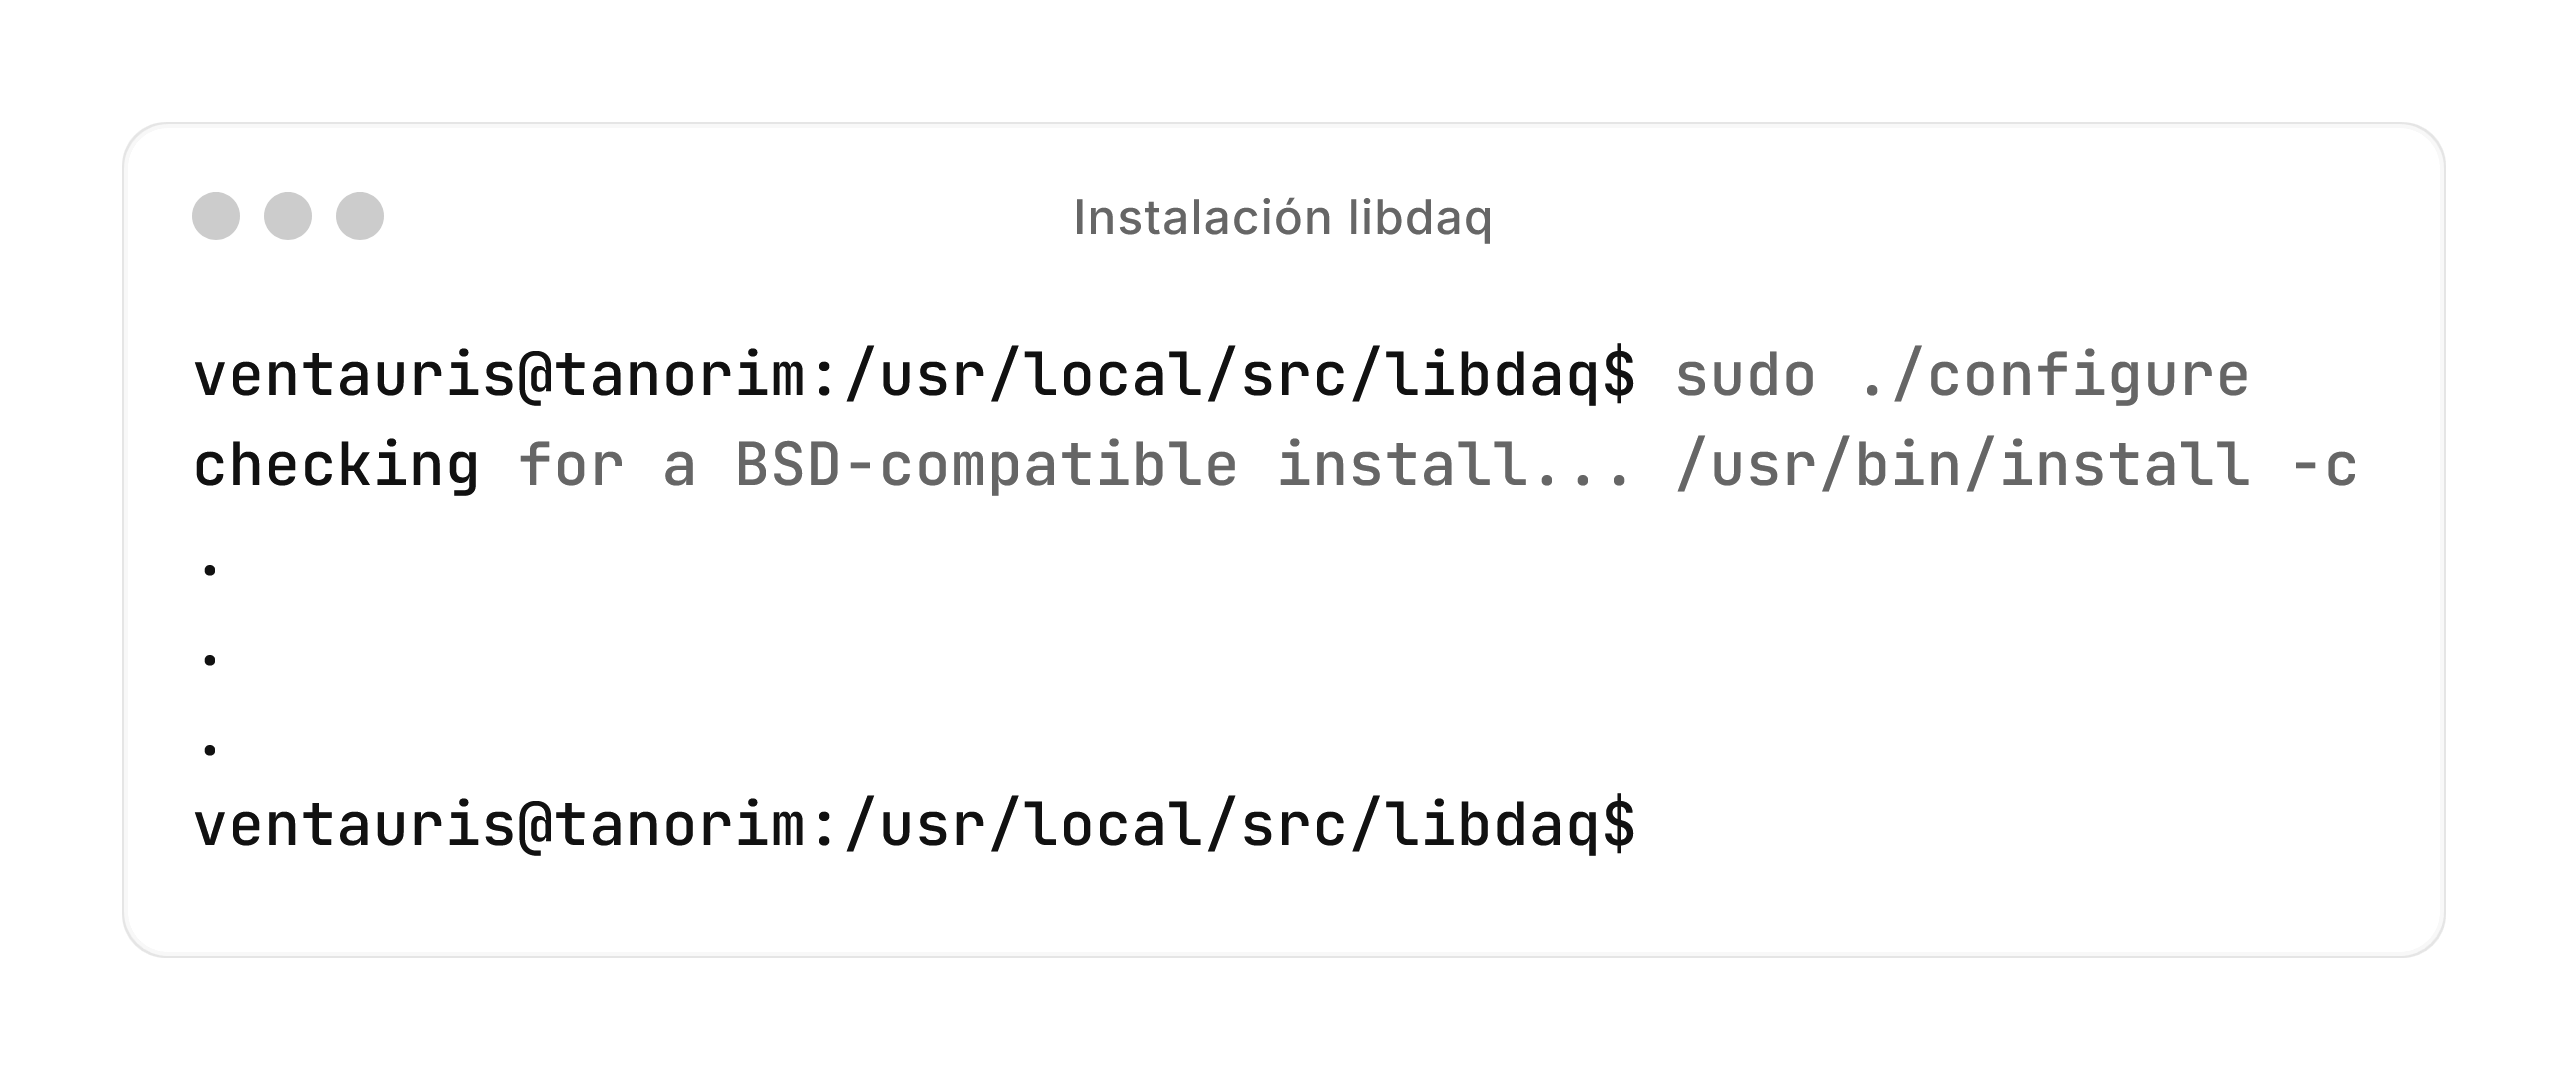
\includegraphics[scale=0.12]{instalacion_snort/11-11.png}
	\caption{Configurando \texttt{libdaq} antes de la compilación.}
\end{figure}

La ejecución de \texttt{make} llevará a cabo la compilación de \texttt{libdaq}. Este proceso traduce el código fuente a binarios ejecutables, asegurándose de que todas las dependencias y archivos necesarios se generen correctamente para su posterior instalación.

\begin{figure}[H]
	\centering
	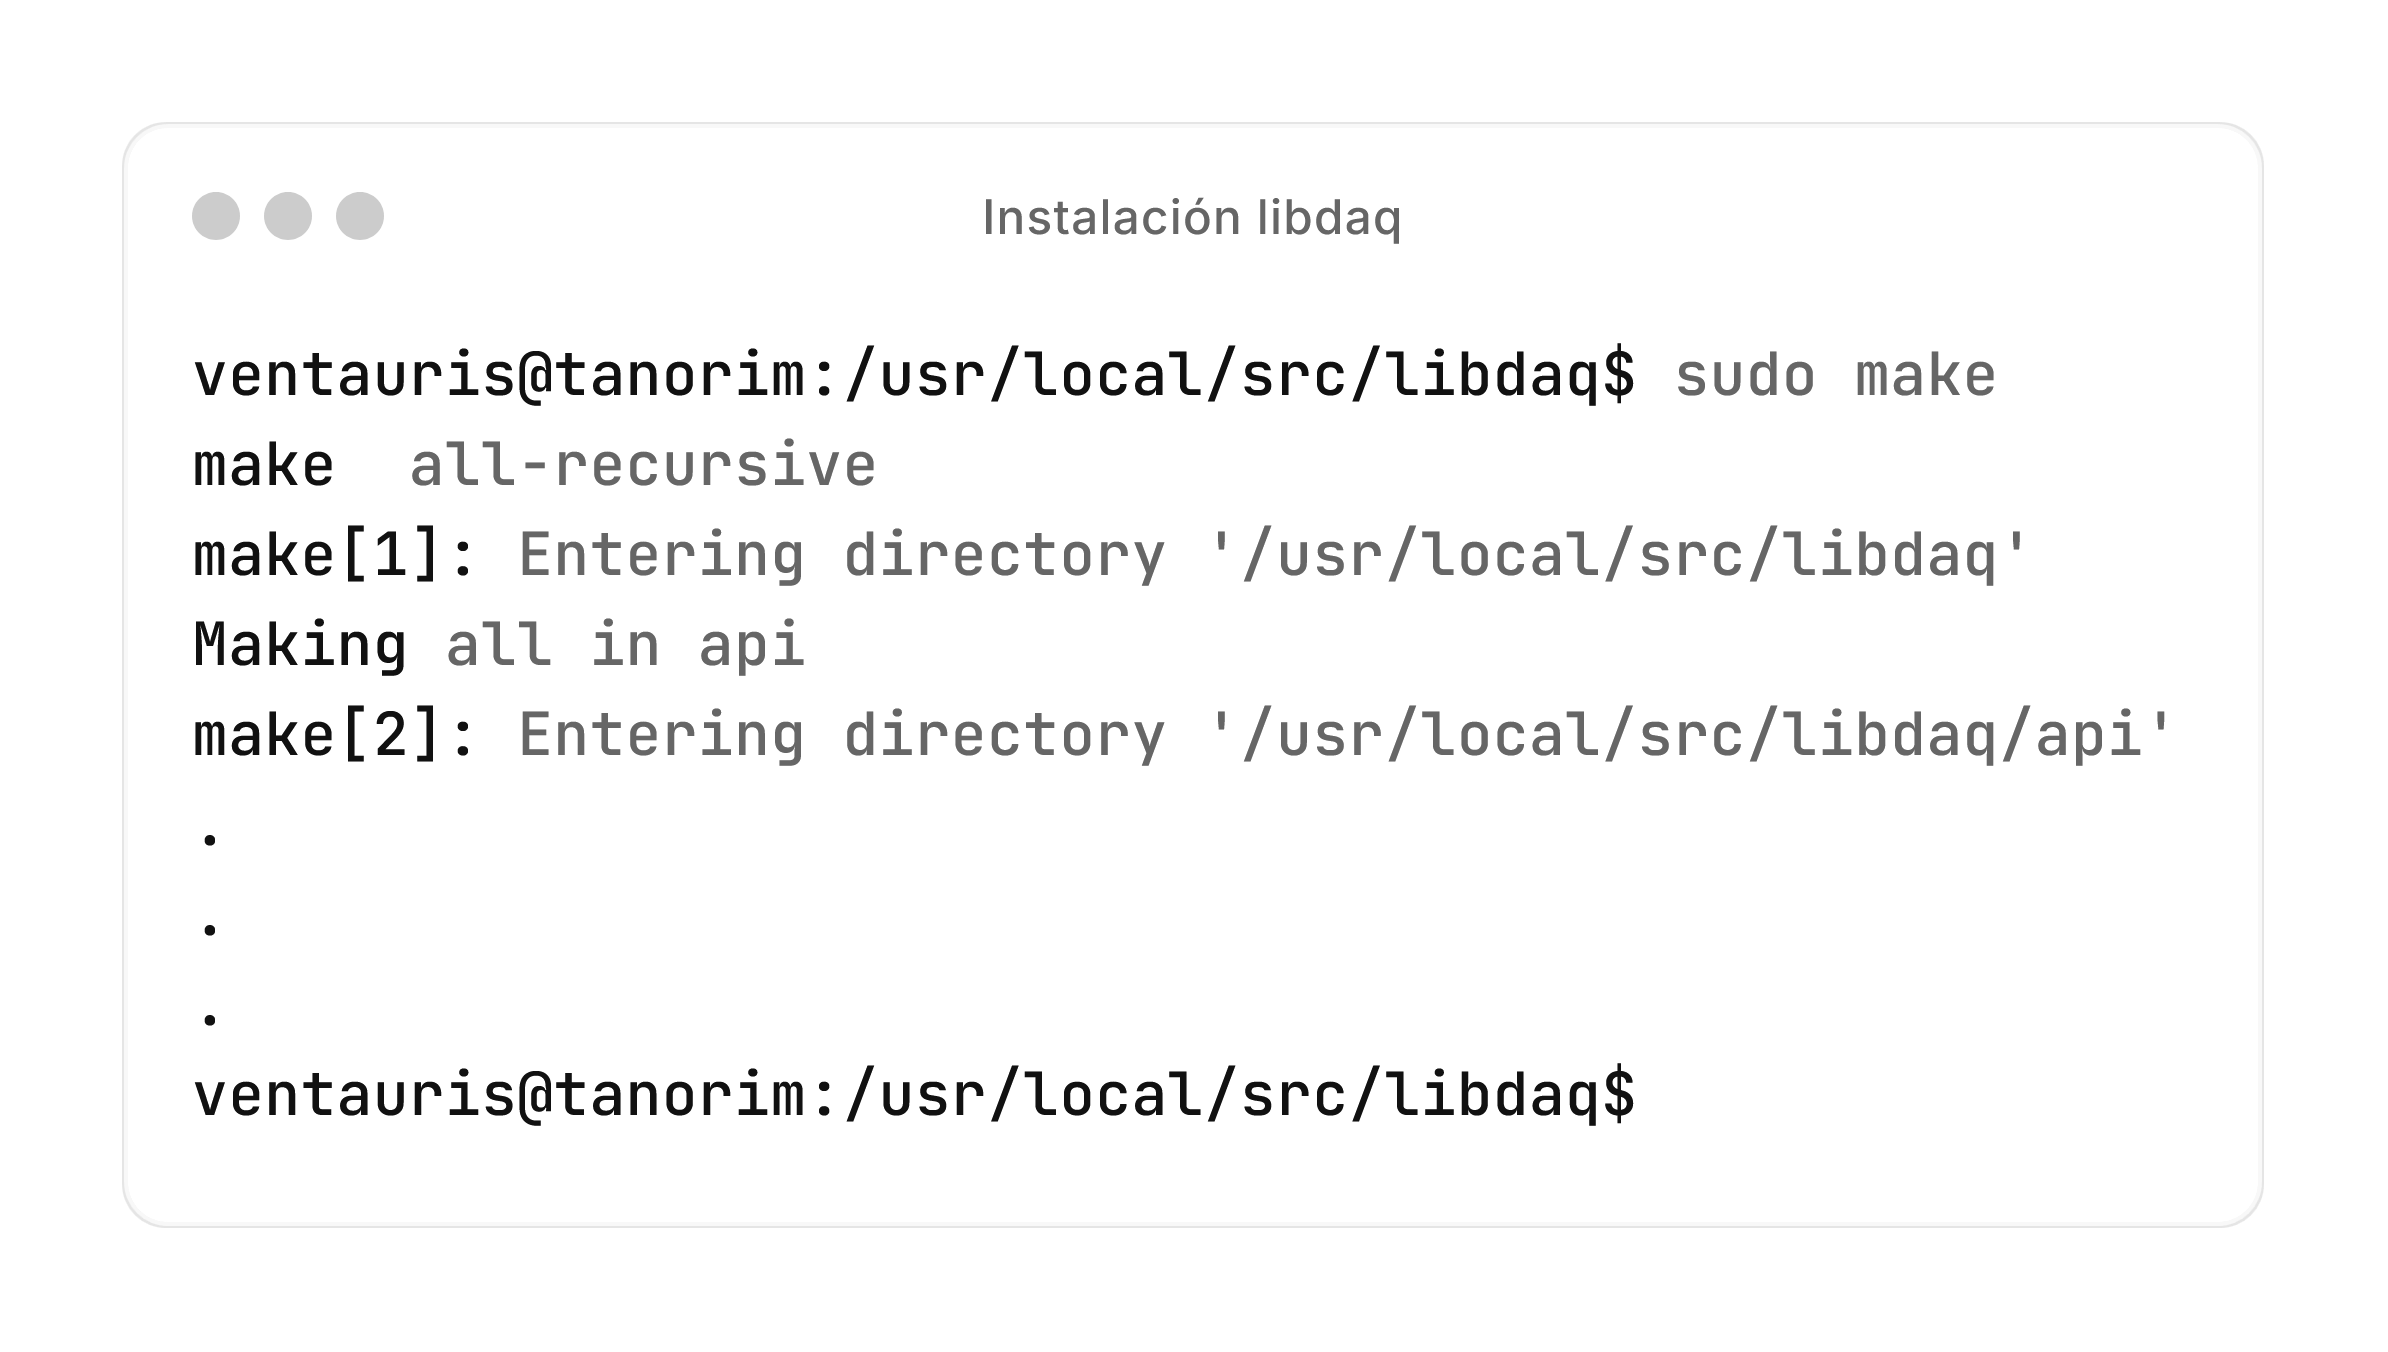
\includegraphics[scale=0.12]{instalacion_snort/12-12.png}
	\caption{Compilando \texttt{libdaq}.}
\end{figure}

\newpage

La instalación final la llevaremos a cabo mediante \texttt{sudo make install}. Esto copia los archivos compilados a sus ubicaciones correspondientes dentro del sistema para que puedan ser utilizados por \textbf{Snort} y otros programas que así lo requieran.

\begin{figure}[H]
	\centering
	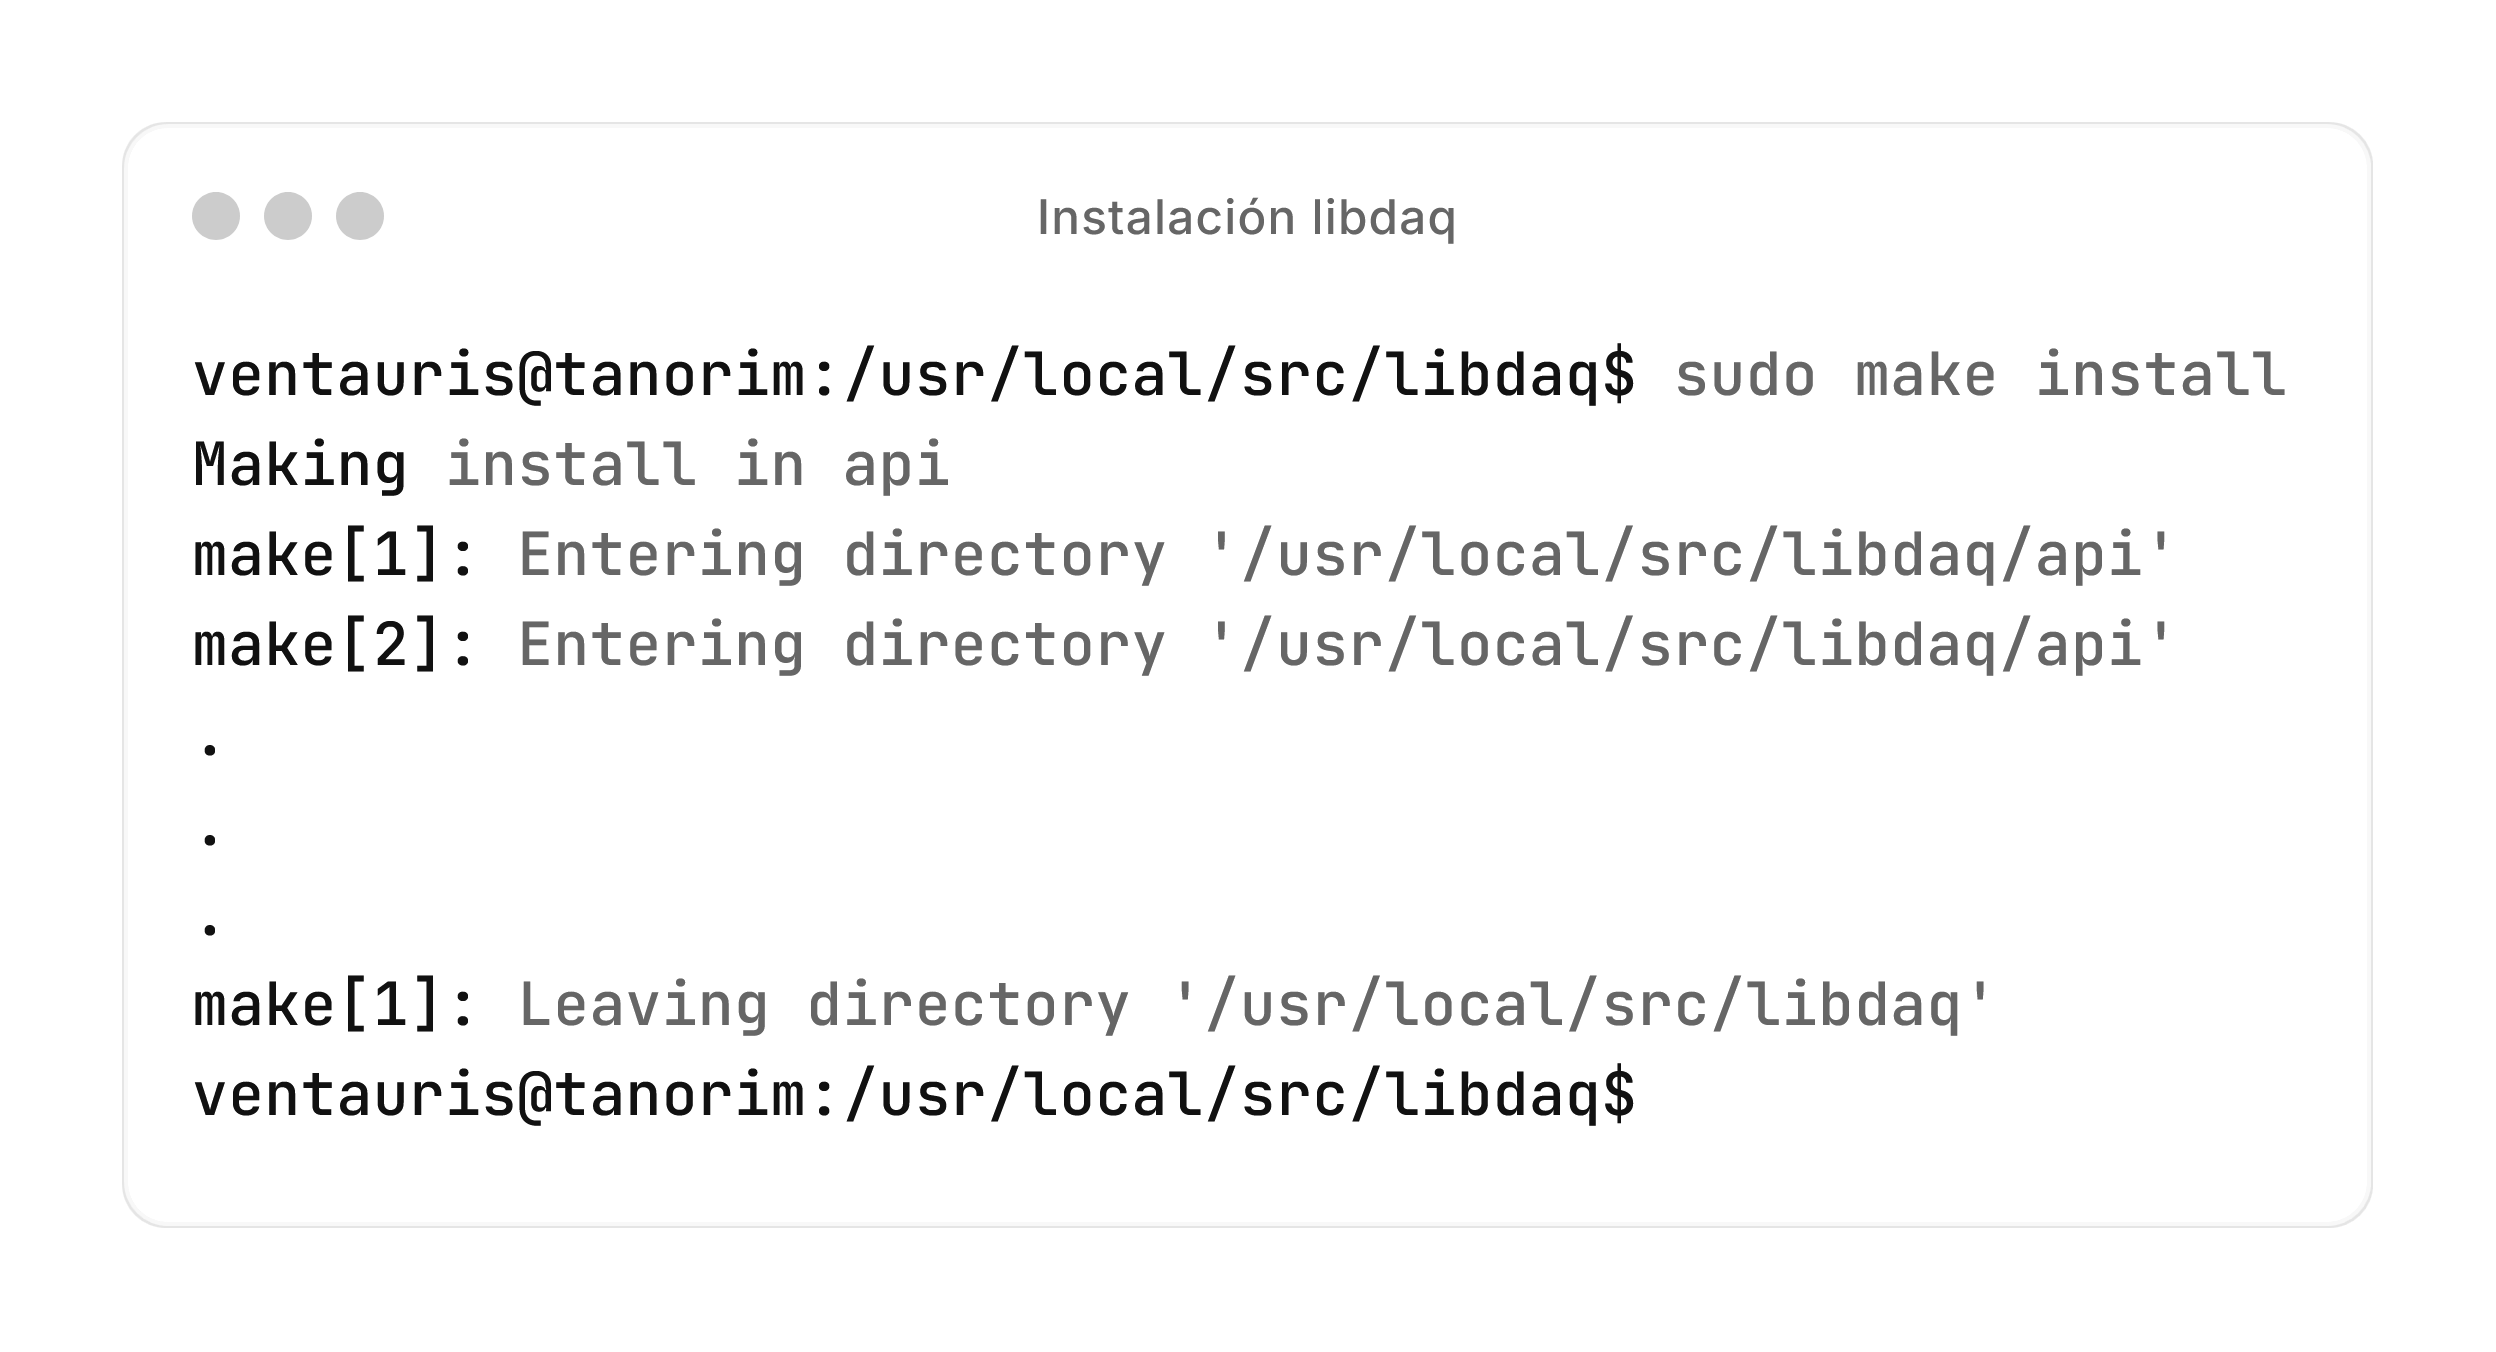
\includegraphics[scale=0.12]{instalacion_snort/13-13.png}
	\caption{Instalando \texttt{libdaq}.}
\end{figure}

Listamos los archivos de configuración de \texttt{libdaq} en \texttt{/usr/local/lib/pkgconfig/} para asegurarnos de que la instalación se haya completado correctamente. Después, exportamos la variable \texttt{PKG\_CONFIG\_PATH} para que el sistema reconozca la librería. Finalmente, usamos \texttt{pkg-config --modversion libdaq} para confirmar que la versión instalada es la \textbf{3.0.19}.

\begin{figure}[H]
	\centering
	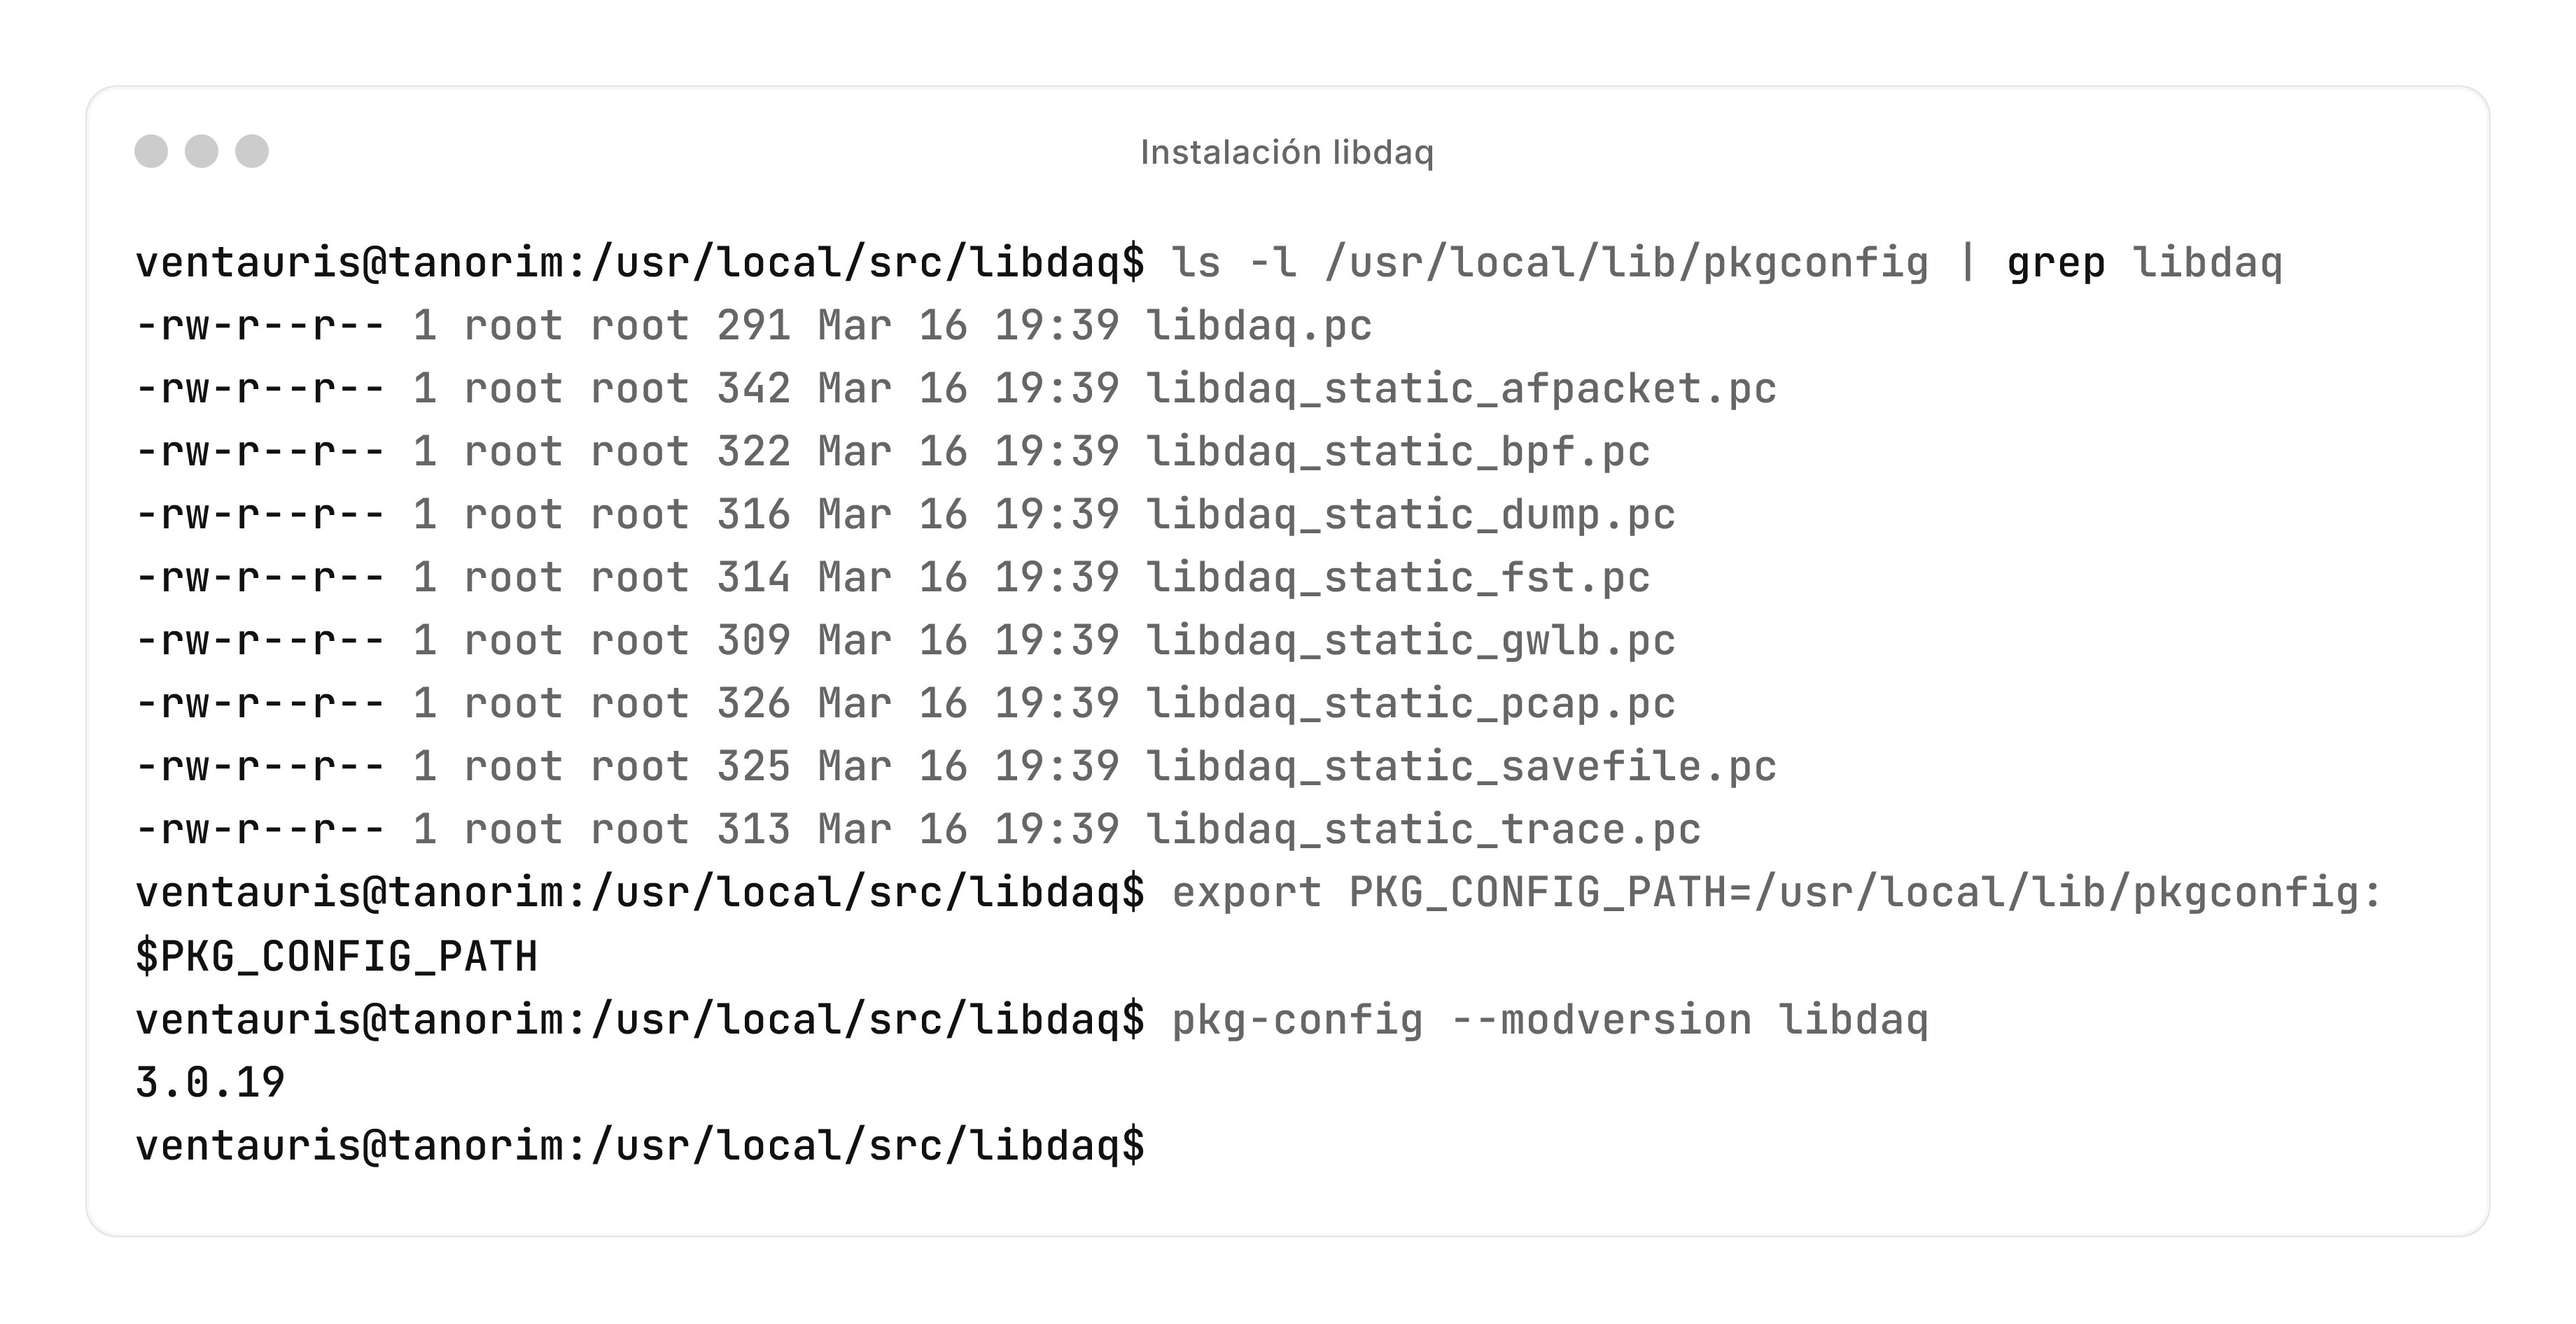
\includegraphics[scale=0.12]{instalacion_snort/14-14.png}
	\caption{Verificando la instalación de \texttt{libdaq}.}
\end{figure}

\newpage

Instalamos \texttt{libhwloc-dev}, una librería necesaria para la ejecución de \textbf{Snort 3} y sus dependencias. Se incluyen automáticamente otros paquetes adicionales como \texttt{libhwloc-plugins}, \texttt{libnuma-dev} y \texttt{libpciaccess0}, que ayudan en la gestión de hardware y optimización del rendimiento.

\begin{figure}[H]
	\centering
	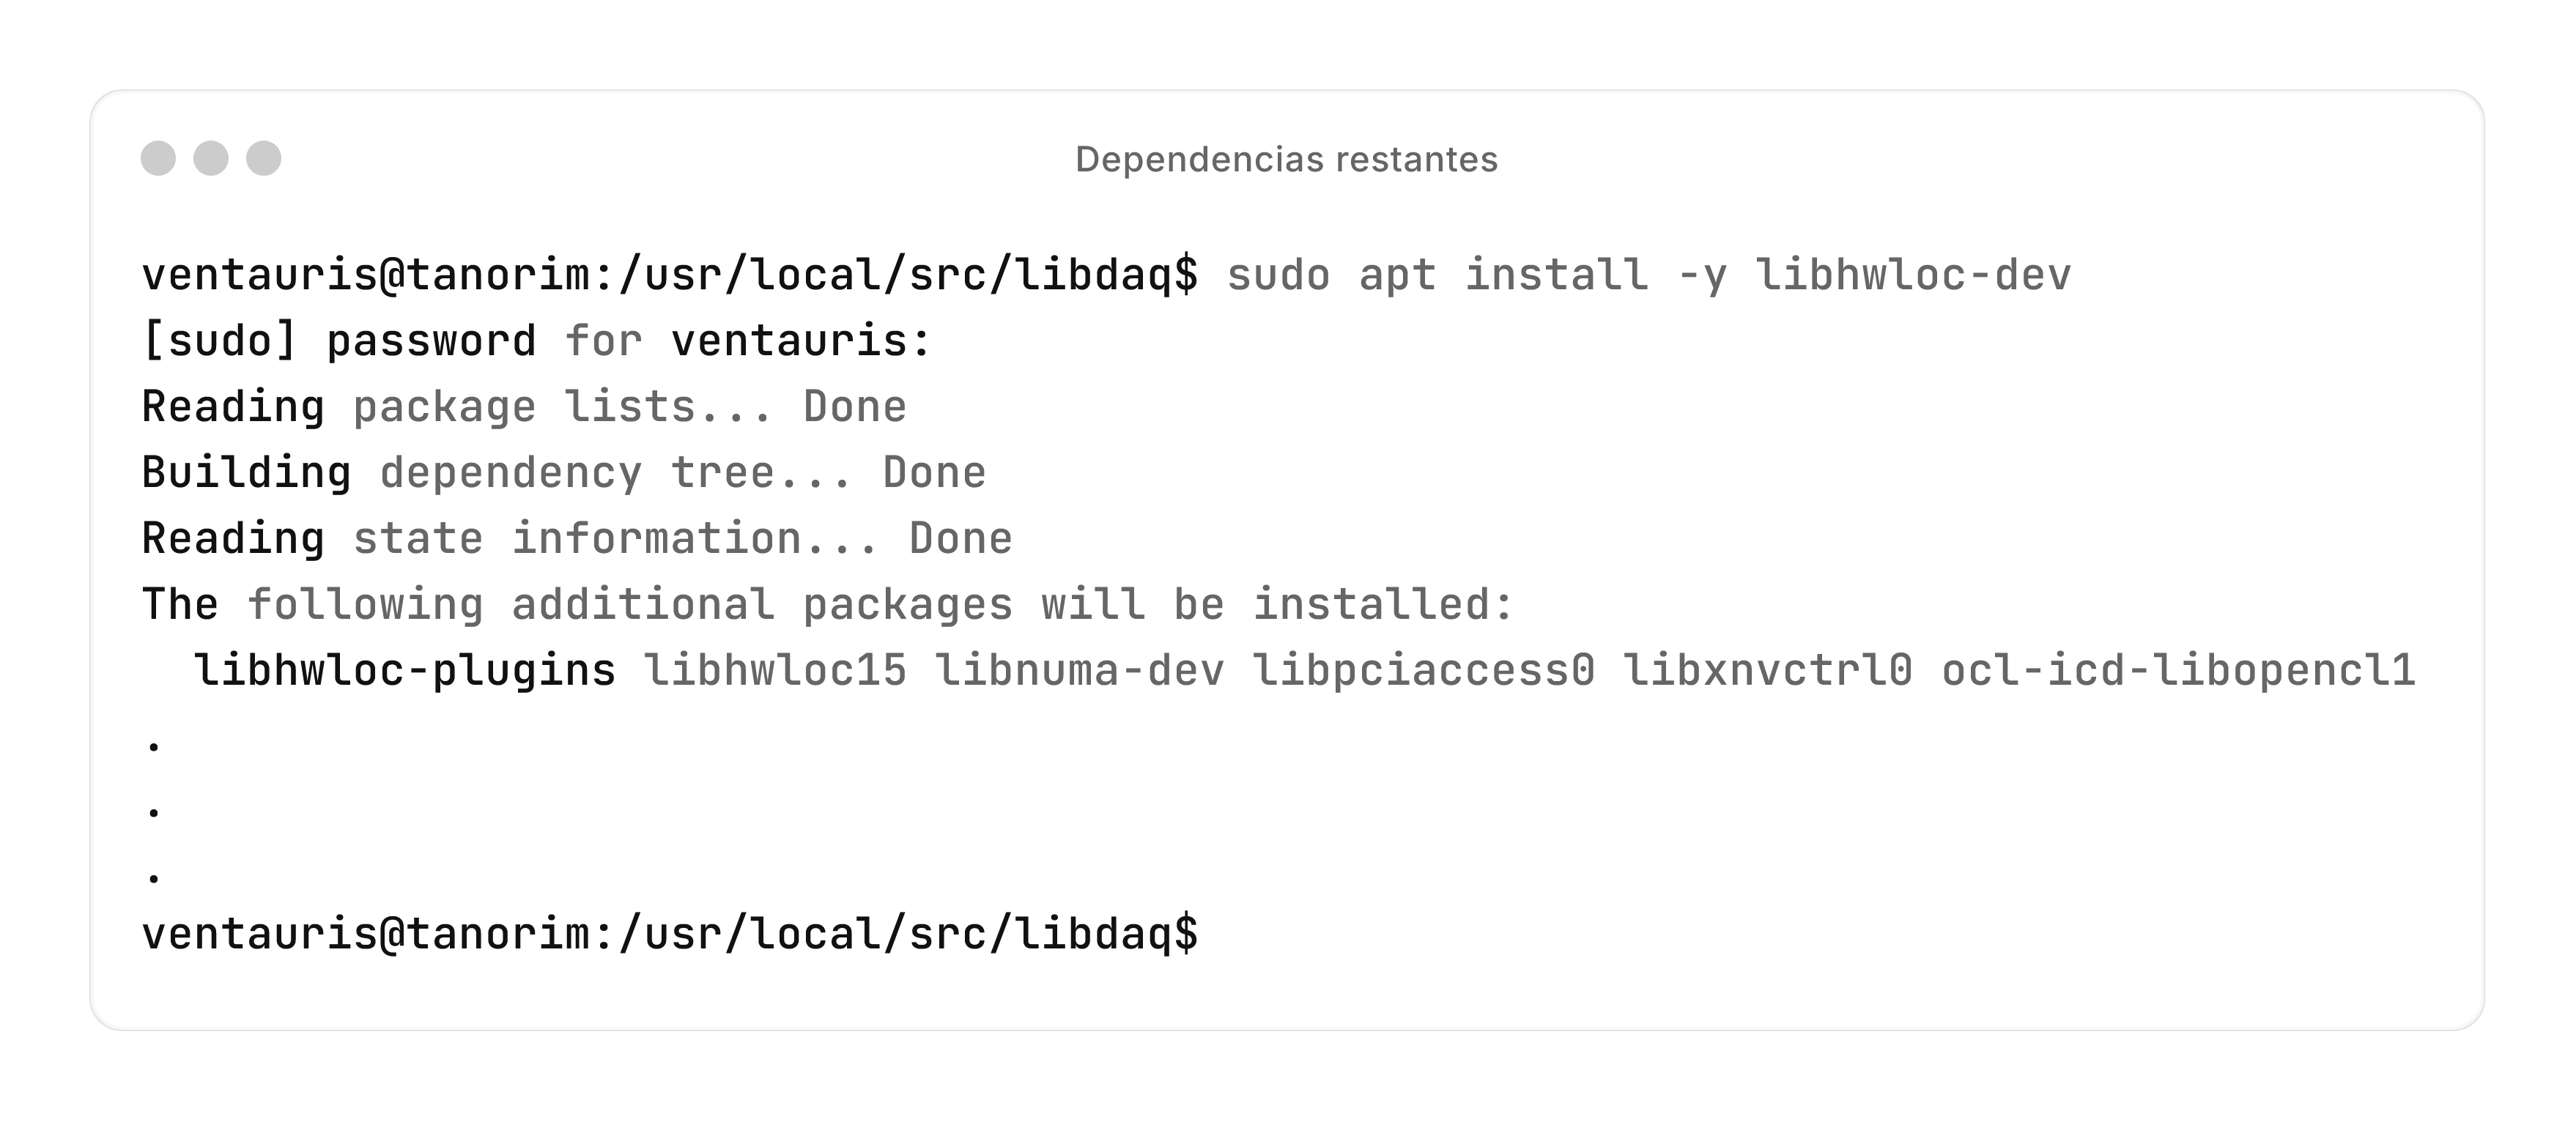
\includegraphics[scale=0.12]{instalacion_snort/15-15.png}
	\caption{Instalando dependencias necesarias.}
\end{figure}

Aquí instalamos \texttt{libluajit-5.1-dev}, más dependencias para \textbf{Snort 3}, ya que utiliza \textbf{LuaJIT} para la configuración y personalización de reglas. También se instalan automáticamente \texttt{libluajit-5.1-2} y \texttt{libluajit-5.1-common}, que contienen las bibliotecas compartidas necesarias para funcionar correctamente.

\begin{figure}[H]
	\centering
	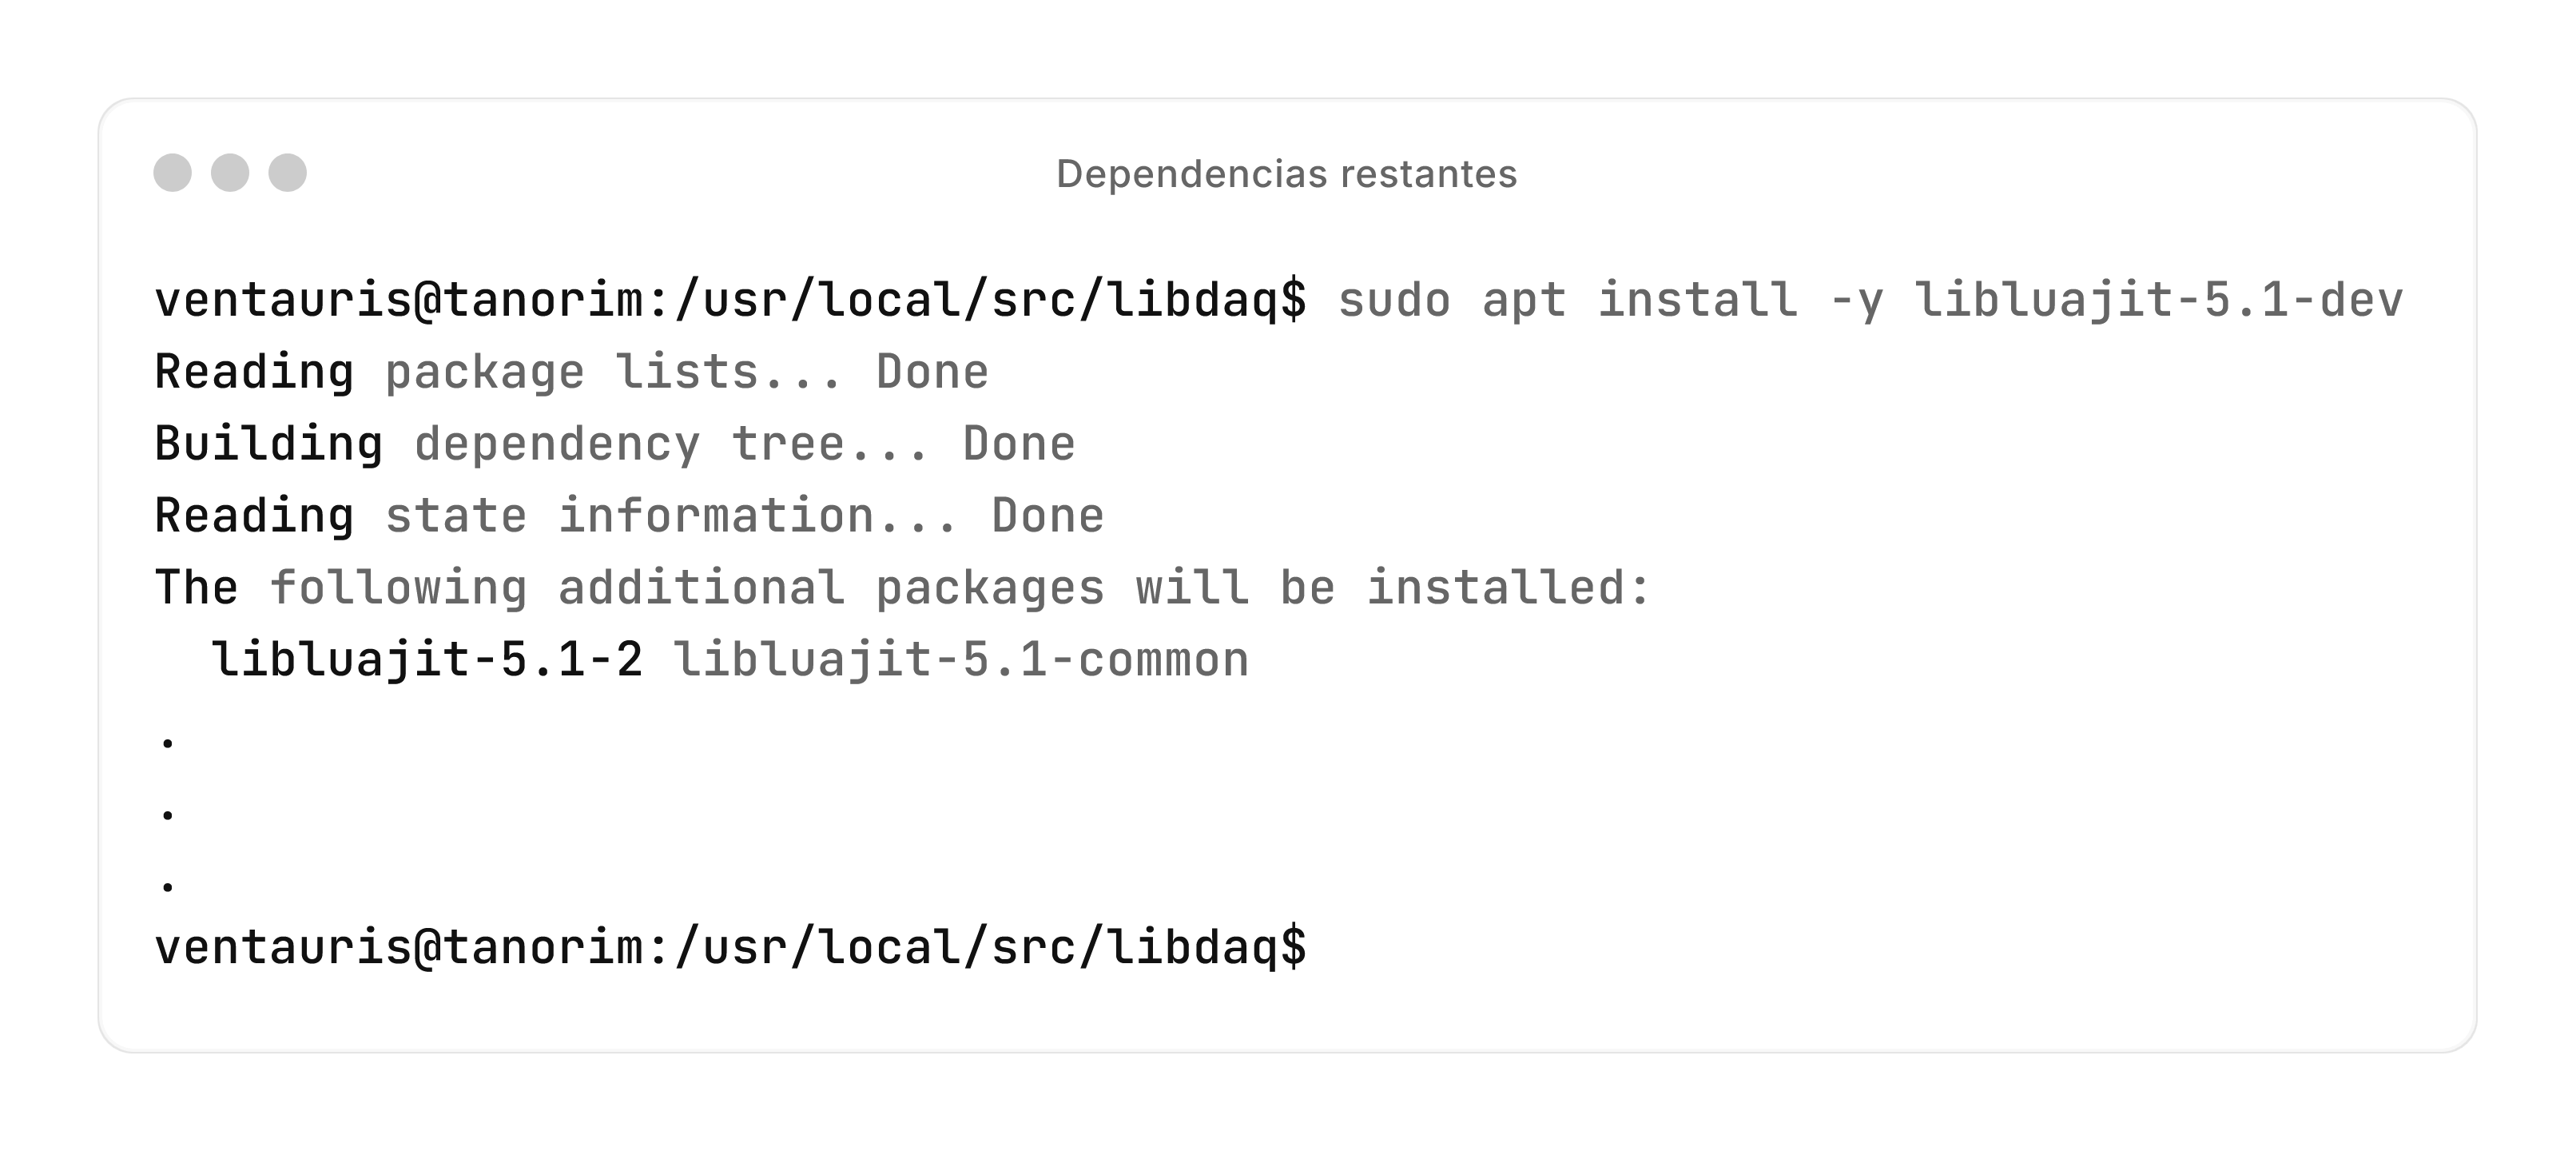
\includegraphics[scale=0.12]{instalacion_snort/16-16.png}
	\caption{Instalando \textbf{LuaJIT} para Snort.}
\end{figure}

\newpage

Descargamos el código fuente de \textbf{Snort 3} directamente desde su repositorio oficial en GitHub mediante \texttt{git clone}.

\begin{figure}[H]
	\centering
	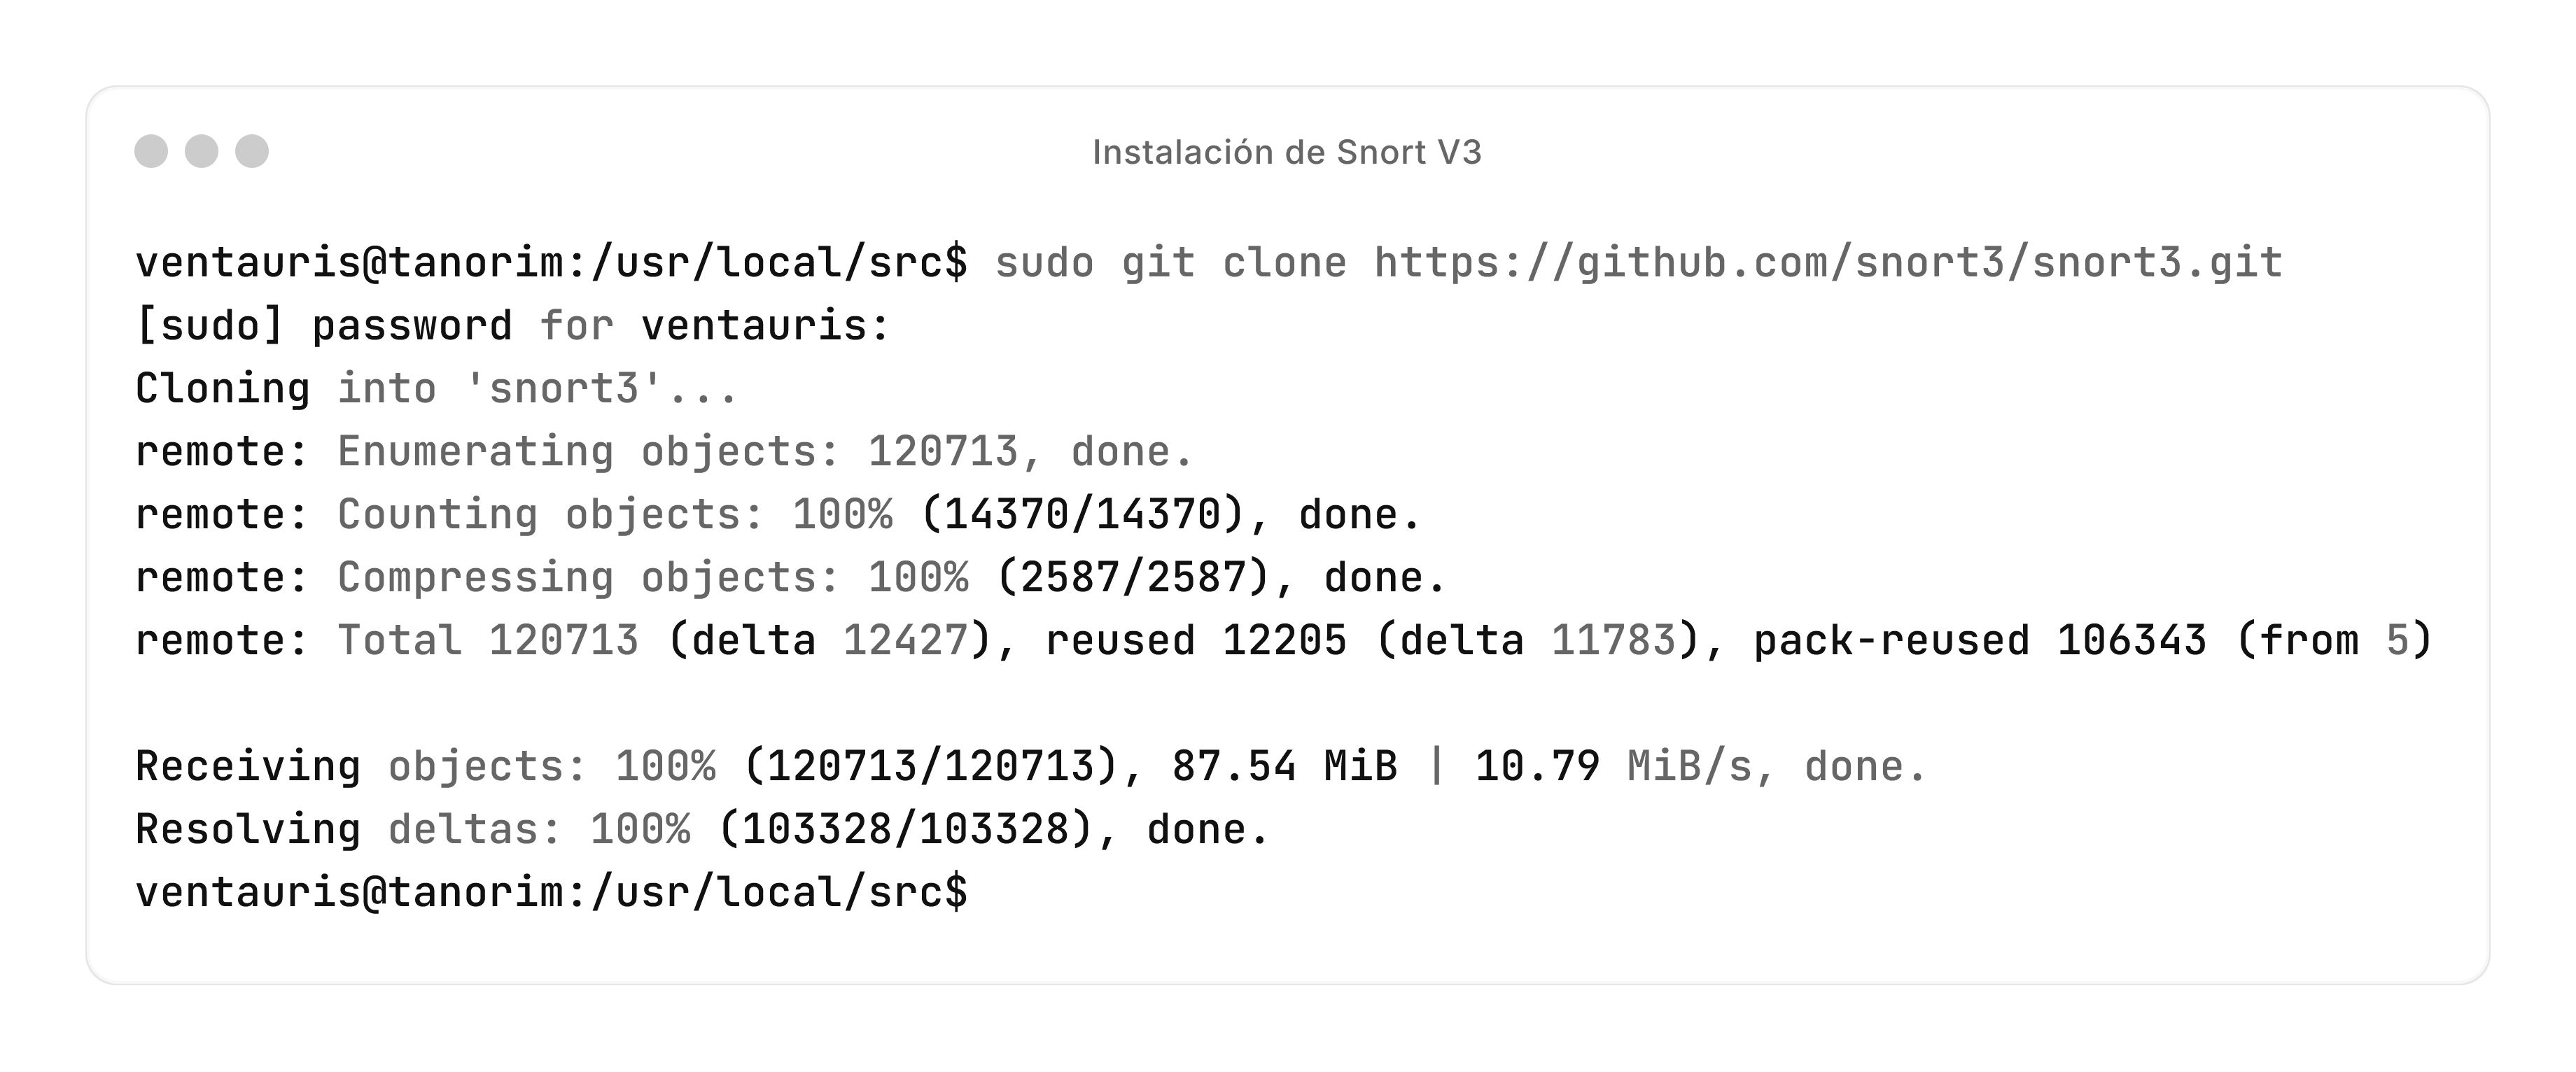
\includegraphics[scale=0.12]{instalacion_snort/17-17.png}
	\caption{Clonando el repositorio de Snort 3.}
\end{figure}

Aquí establecemos la variable \texttt{my\_path} para definir el directorio de instalación de Snort. Luego, agregamos esta configuración al archivo \texttt{~/.bashrc} para que se cargue automáticamente en futuras sesiones. Finalmente, usamos \texttt{source ~/.bashrc} para aplicar los cambios de inmediato.

\begin{figure}[H]
	\centering
	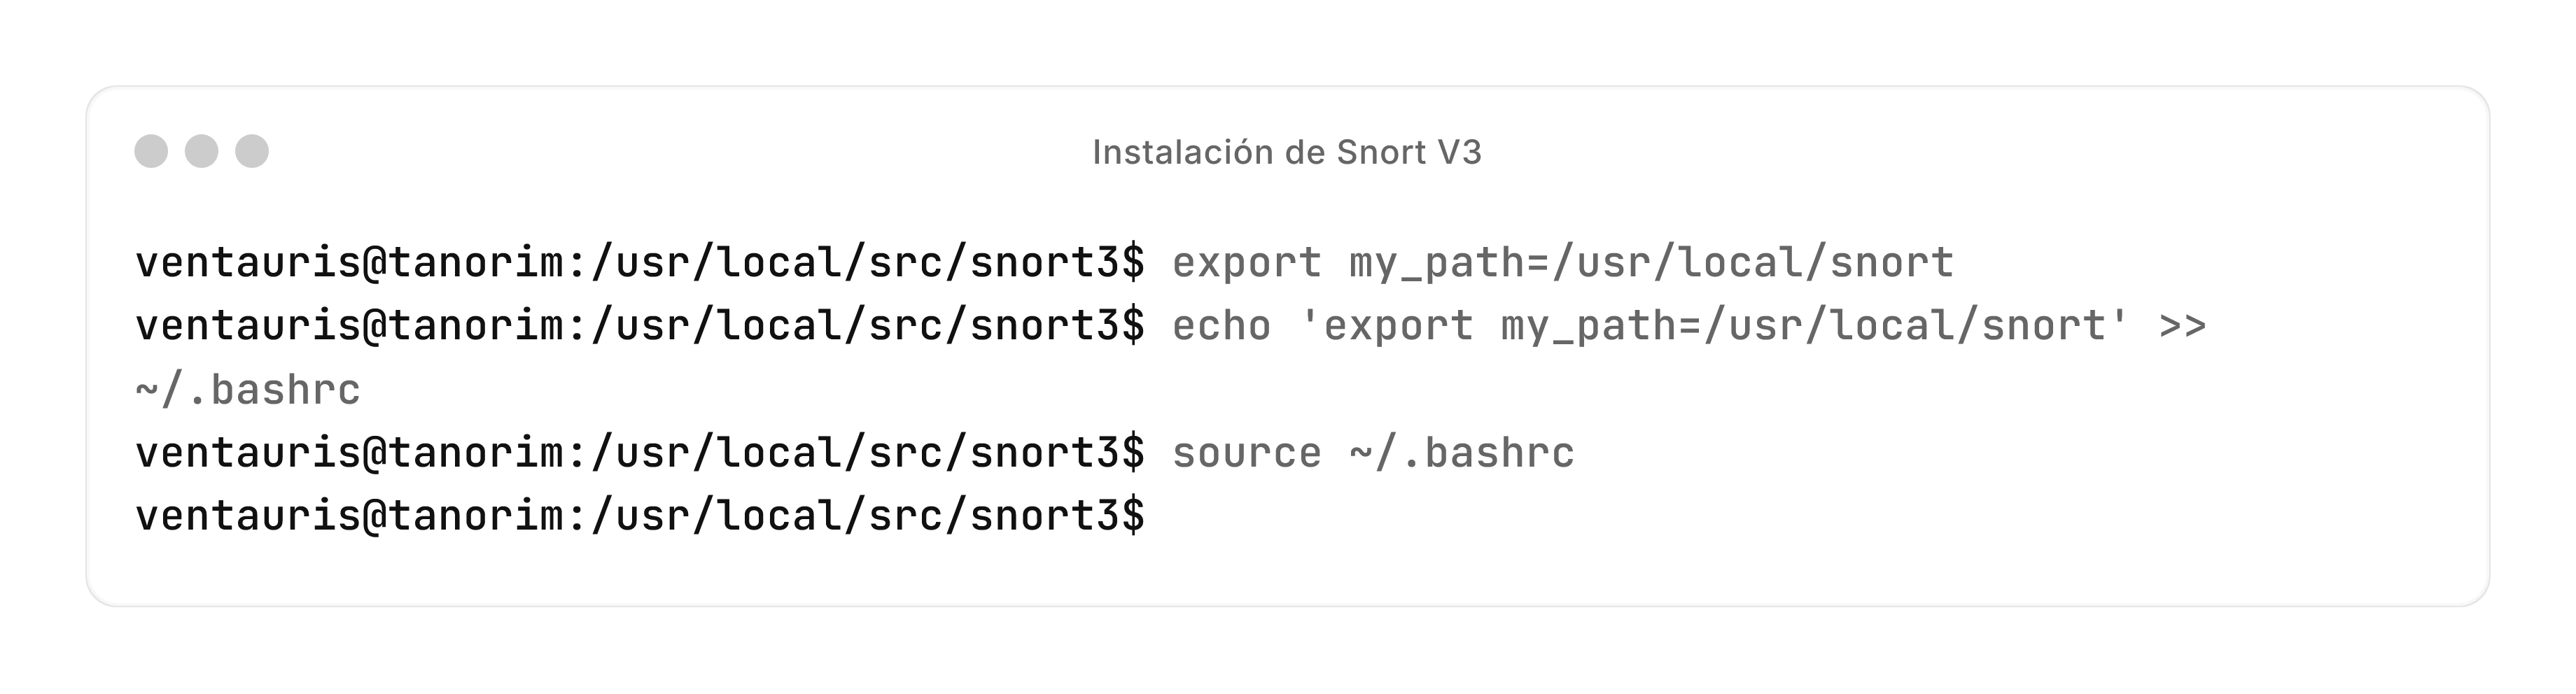
\includegraphics[scale=0.12]{instalacion_snort/18-18.png}
	\caption{Definiendo la ruta de instalación de Snort.}
\end{figure}

\newpage

Instalamos \texttt{Flex} y \texttt{Bison}, dos herramientas para el análisis léxico y sintáctico en la compilación de Snort. Después de la instalación, verificamos la versión de \texttt{Flex} con \texttt{flex --version} para asegurarnos de que se instaló correctamente.

\begin{figure}[H]
	\centering
	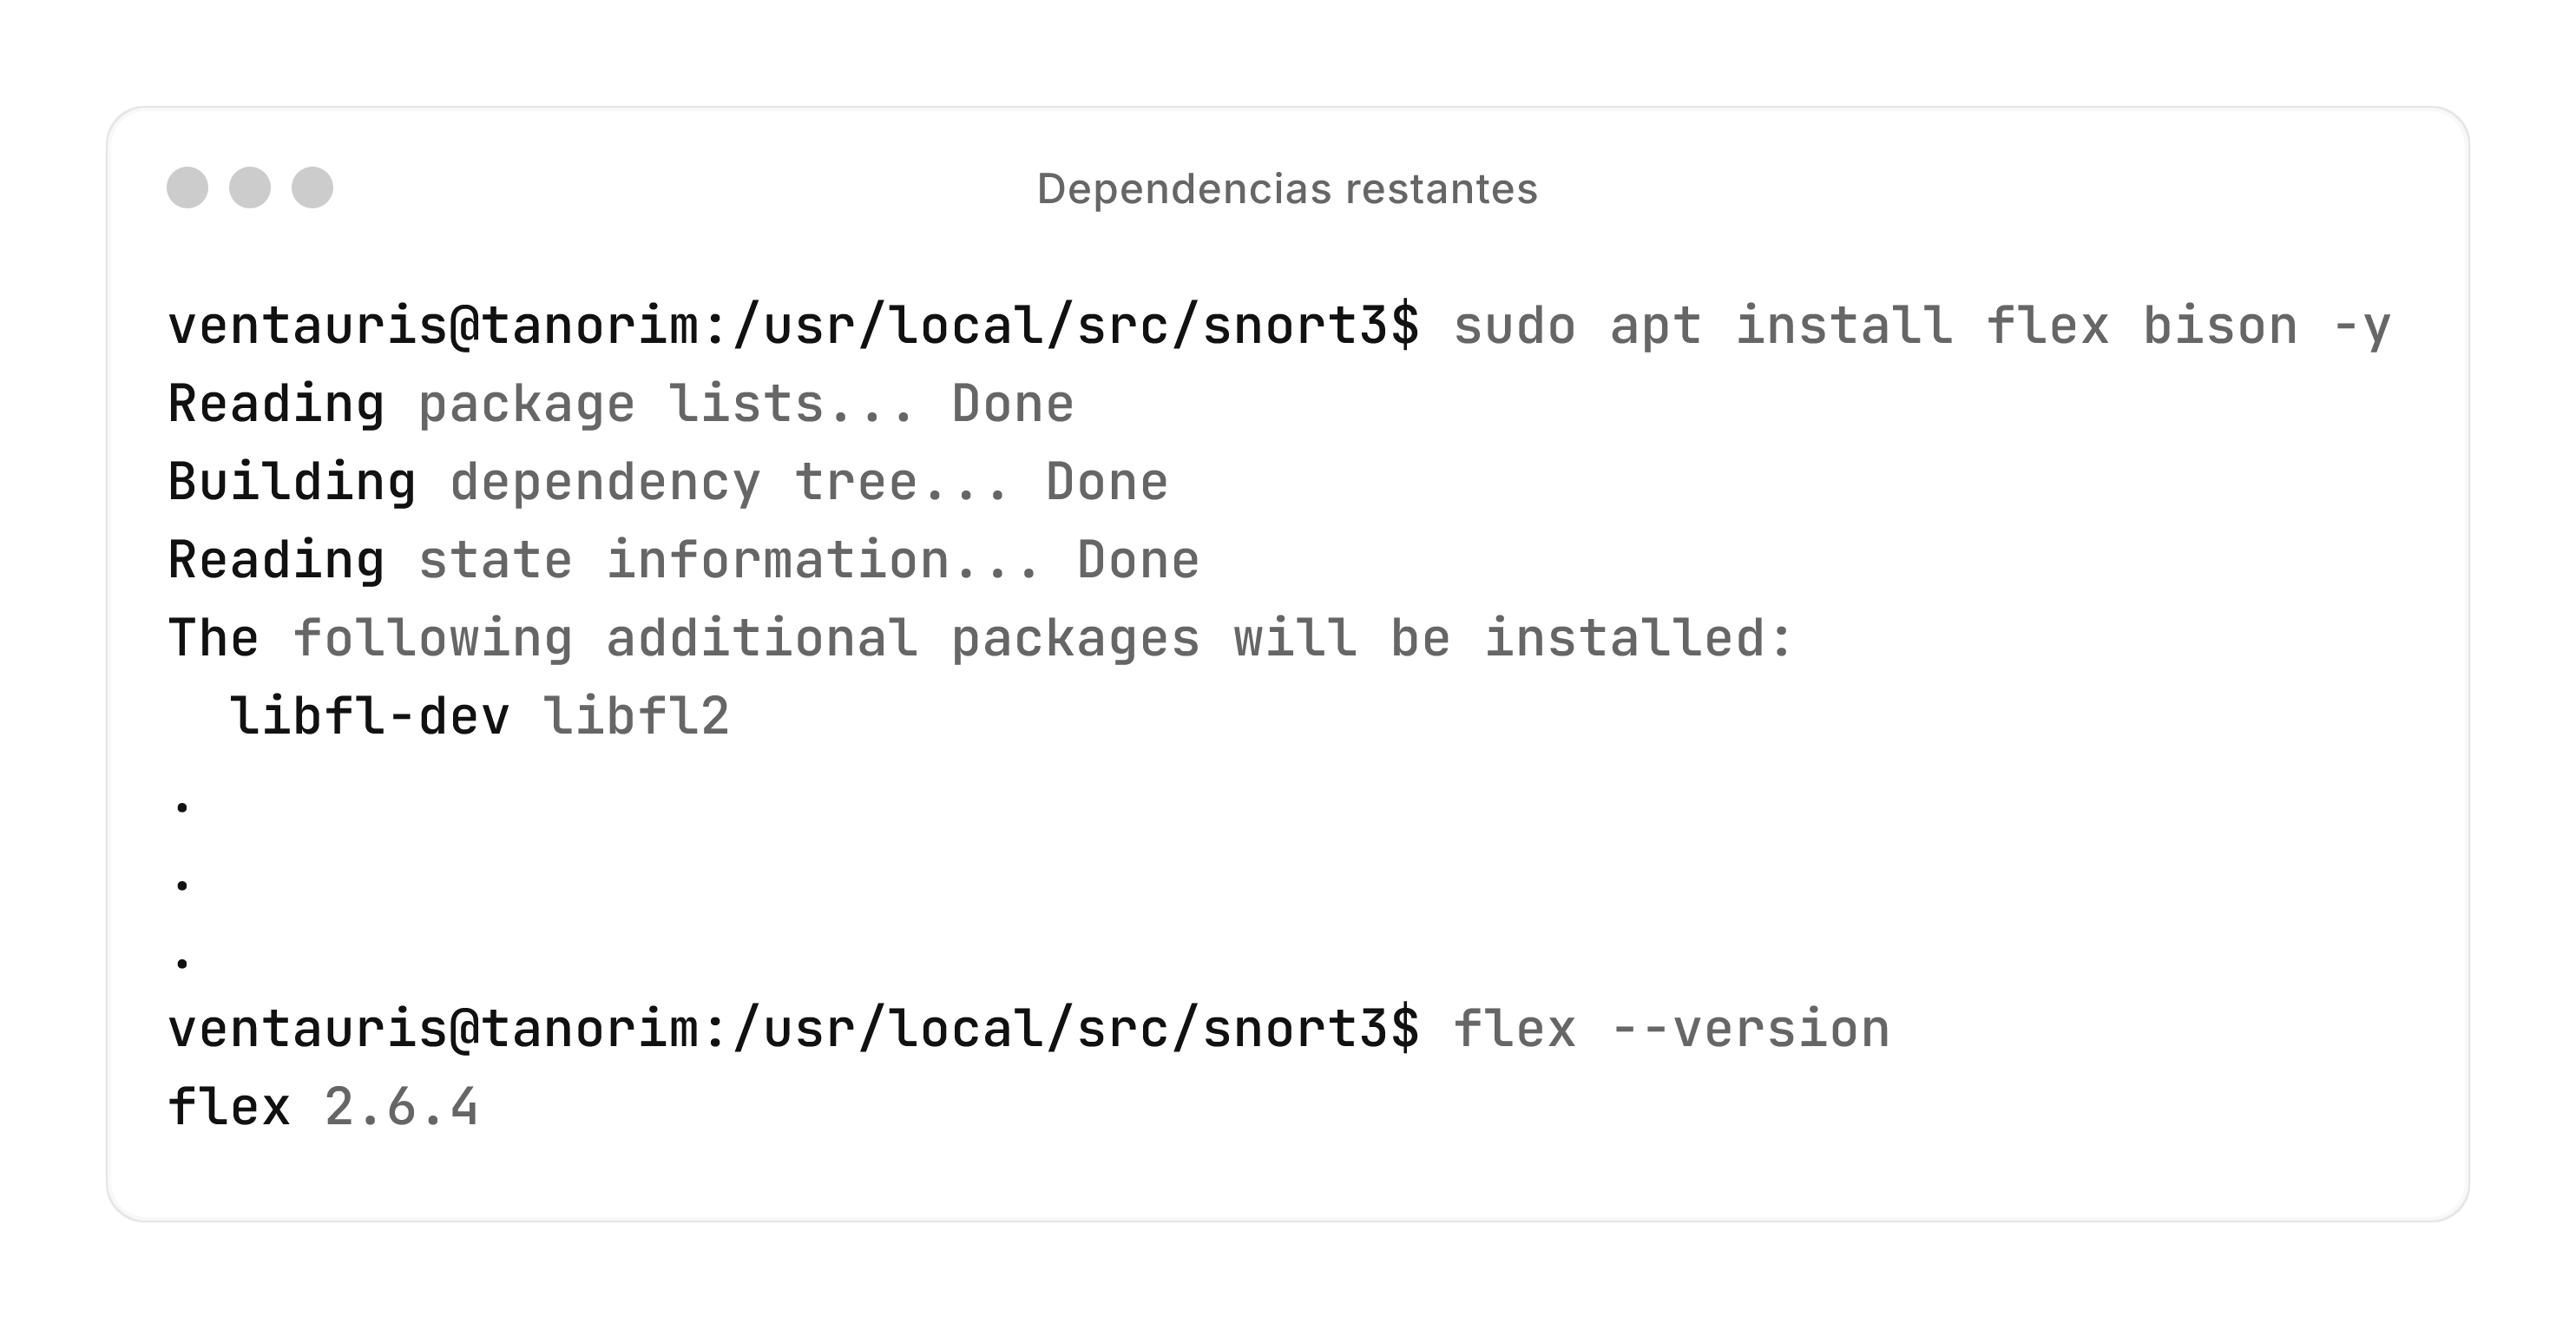
\includegraphics[scale=0.12]{instalacion_snort/19-19.png}
	\caption{Instalando \texttt{Flex} y \texttt{Bison}, herramientas necesarias para la compilación.}
\end{figure}

En este paso, instalamos \texttt{libpcre2-dev}, una biblioteca para el manejo de expresiones regulares en \textbf{Snort 3}. Nos es útil para la detección de patrones en el tráfico de red.

\begin{figure}[H]
	\centering
	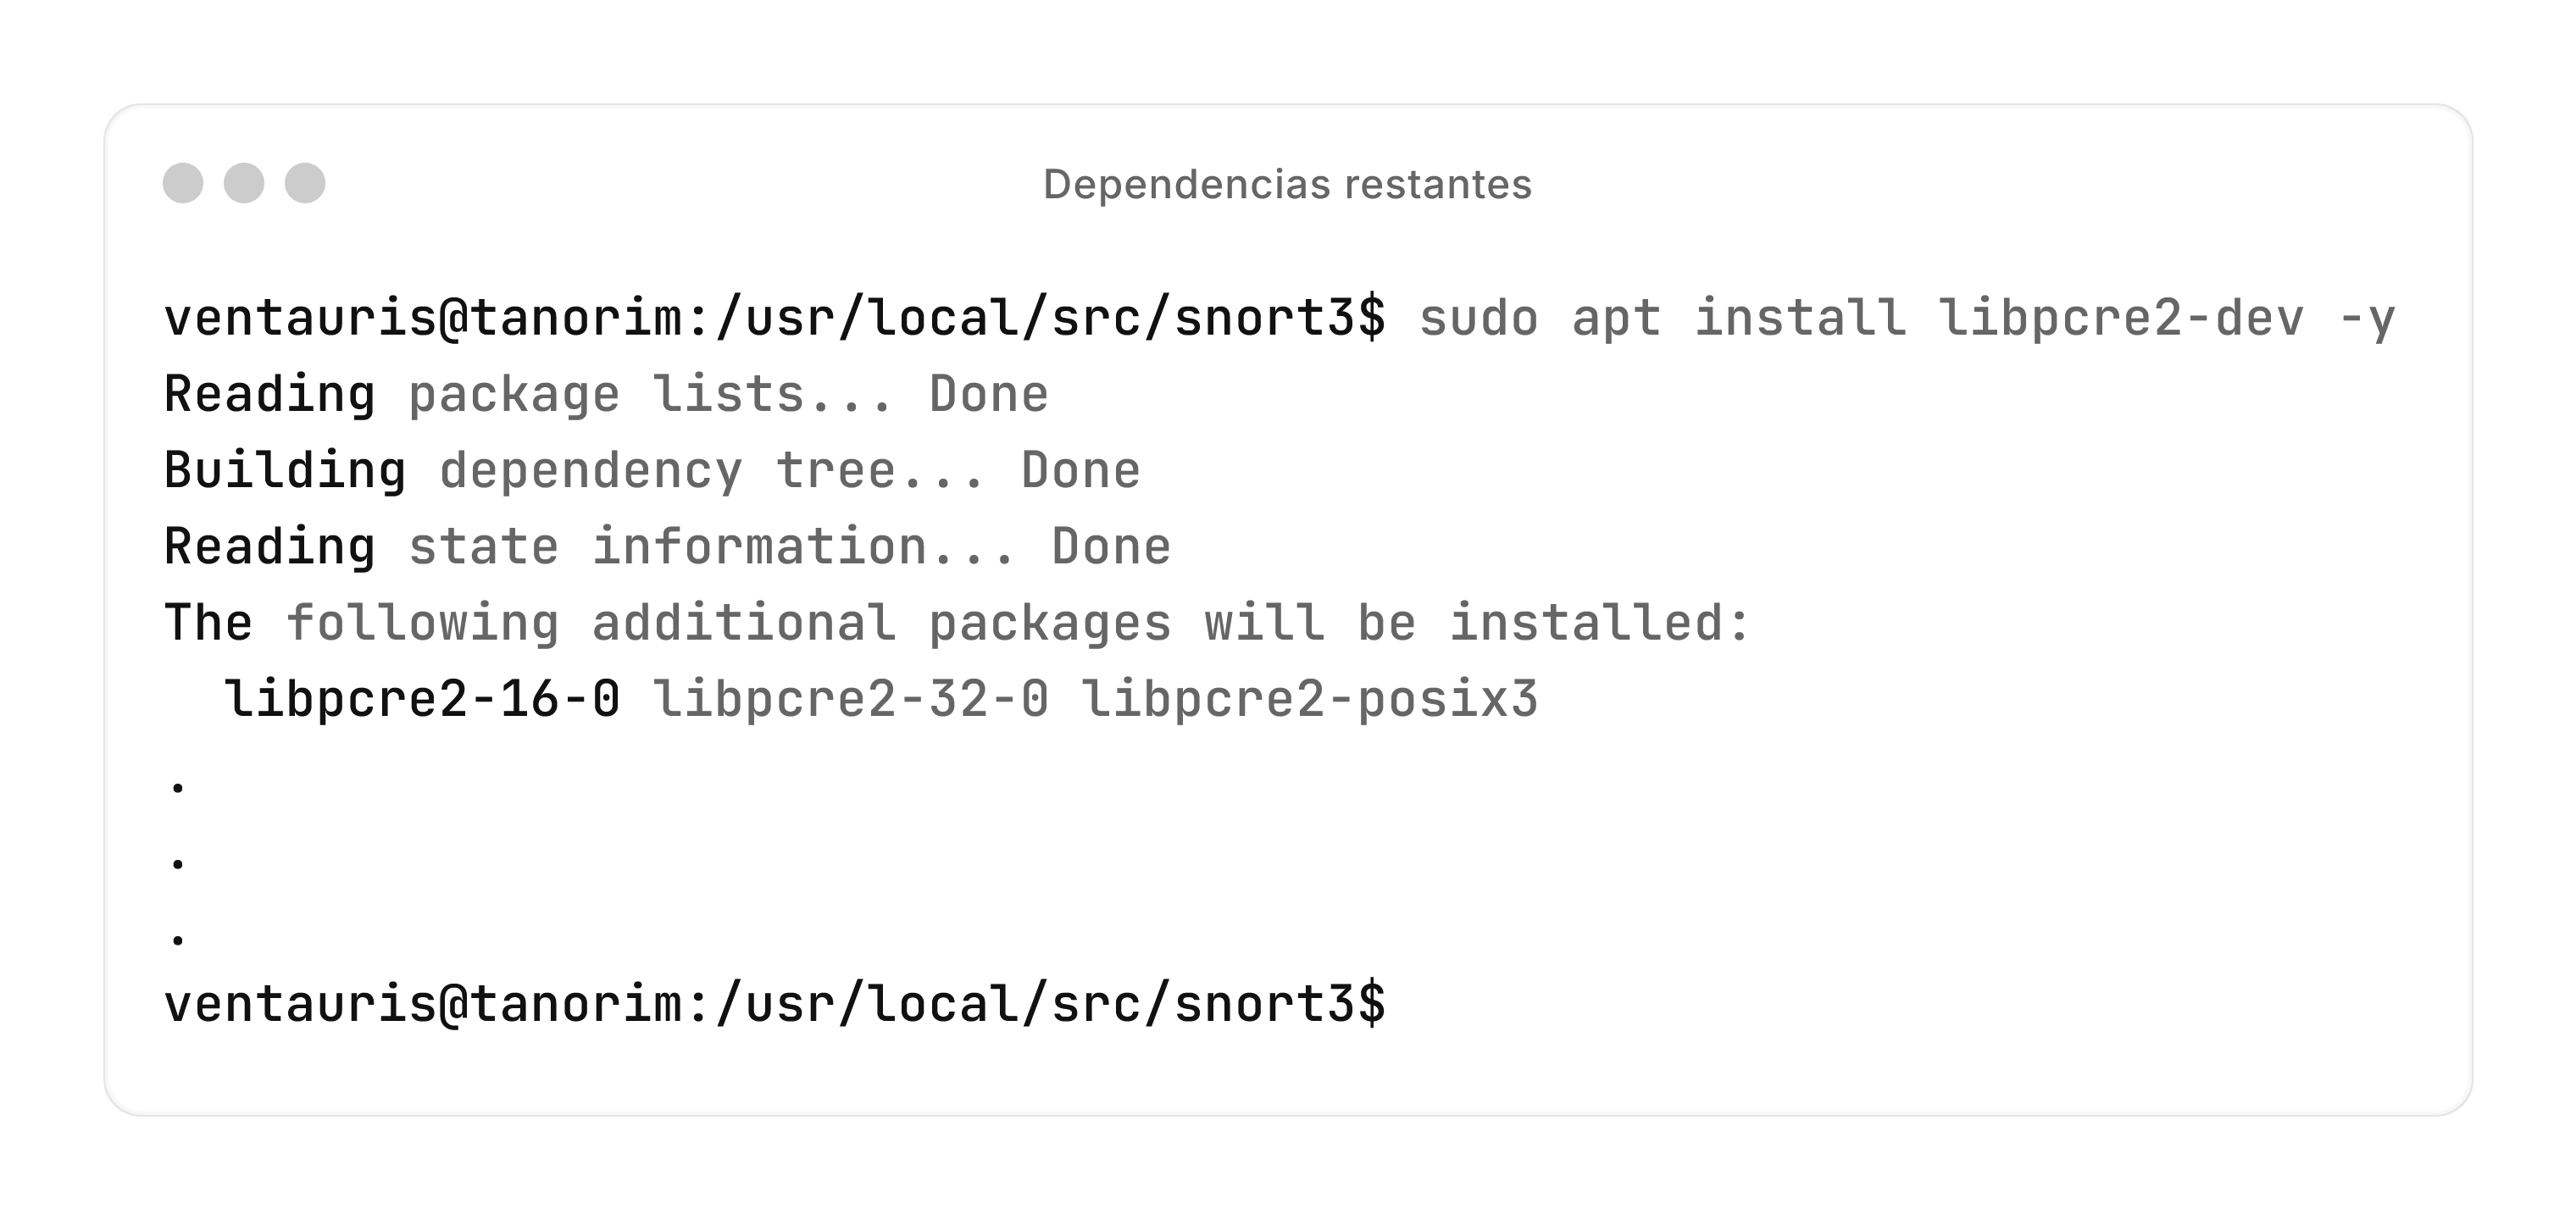
\includegraphics[scale=0.12]{instalacion_snort/20-20.png}
	\caption{Instalando la biblioteca \texttt{PCRE2} para el manejo de expresiones regulares.}
\end{figure}

\newpage

Ejecutamos el script \texttt{configure\_cmake.sh} para configurar la compilación de \textbf{Snort 3}. Se especifica el prefijo de instalación con \texttt{\$my\_path}. Se generan los archivos de configuración y se definen las opciones de características, incluyendo los módulos \texttt{DAQ} que se activarán.

\begin{figure}[H]
	\centering
	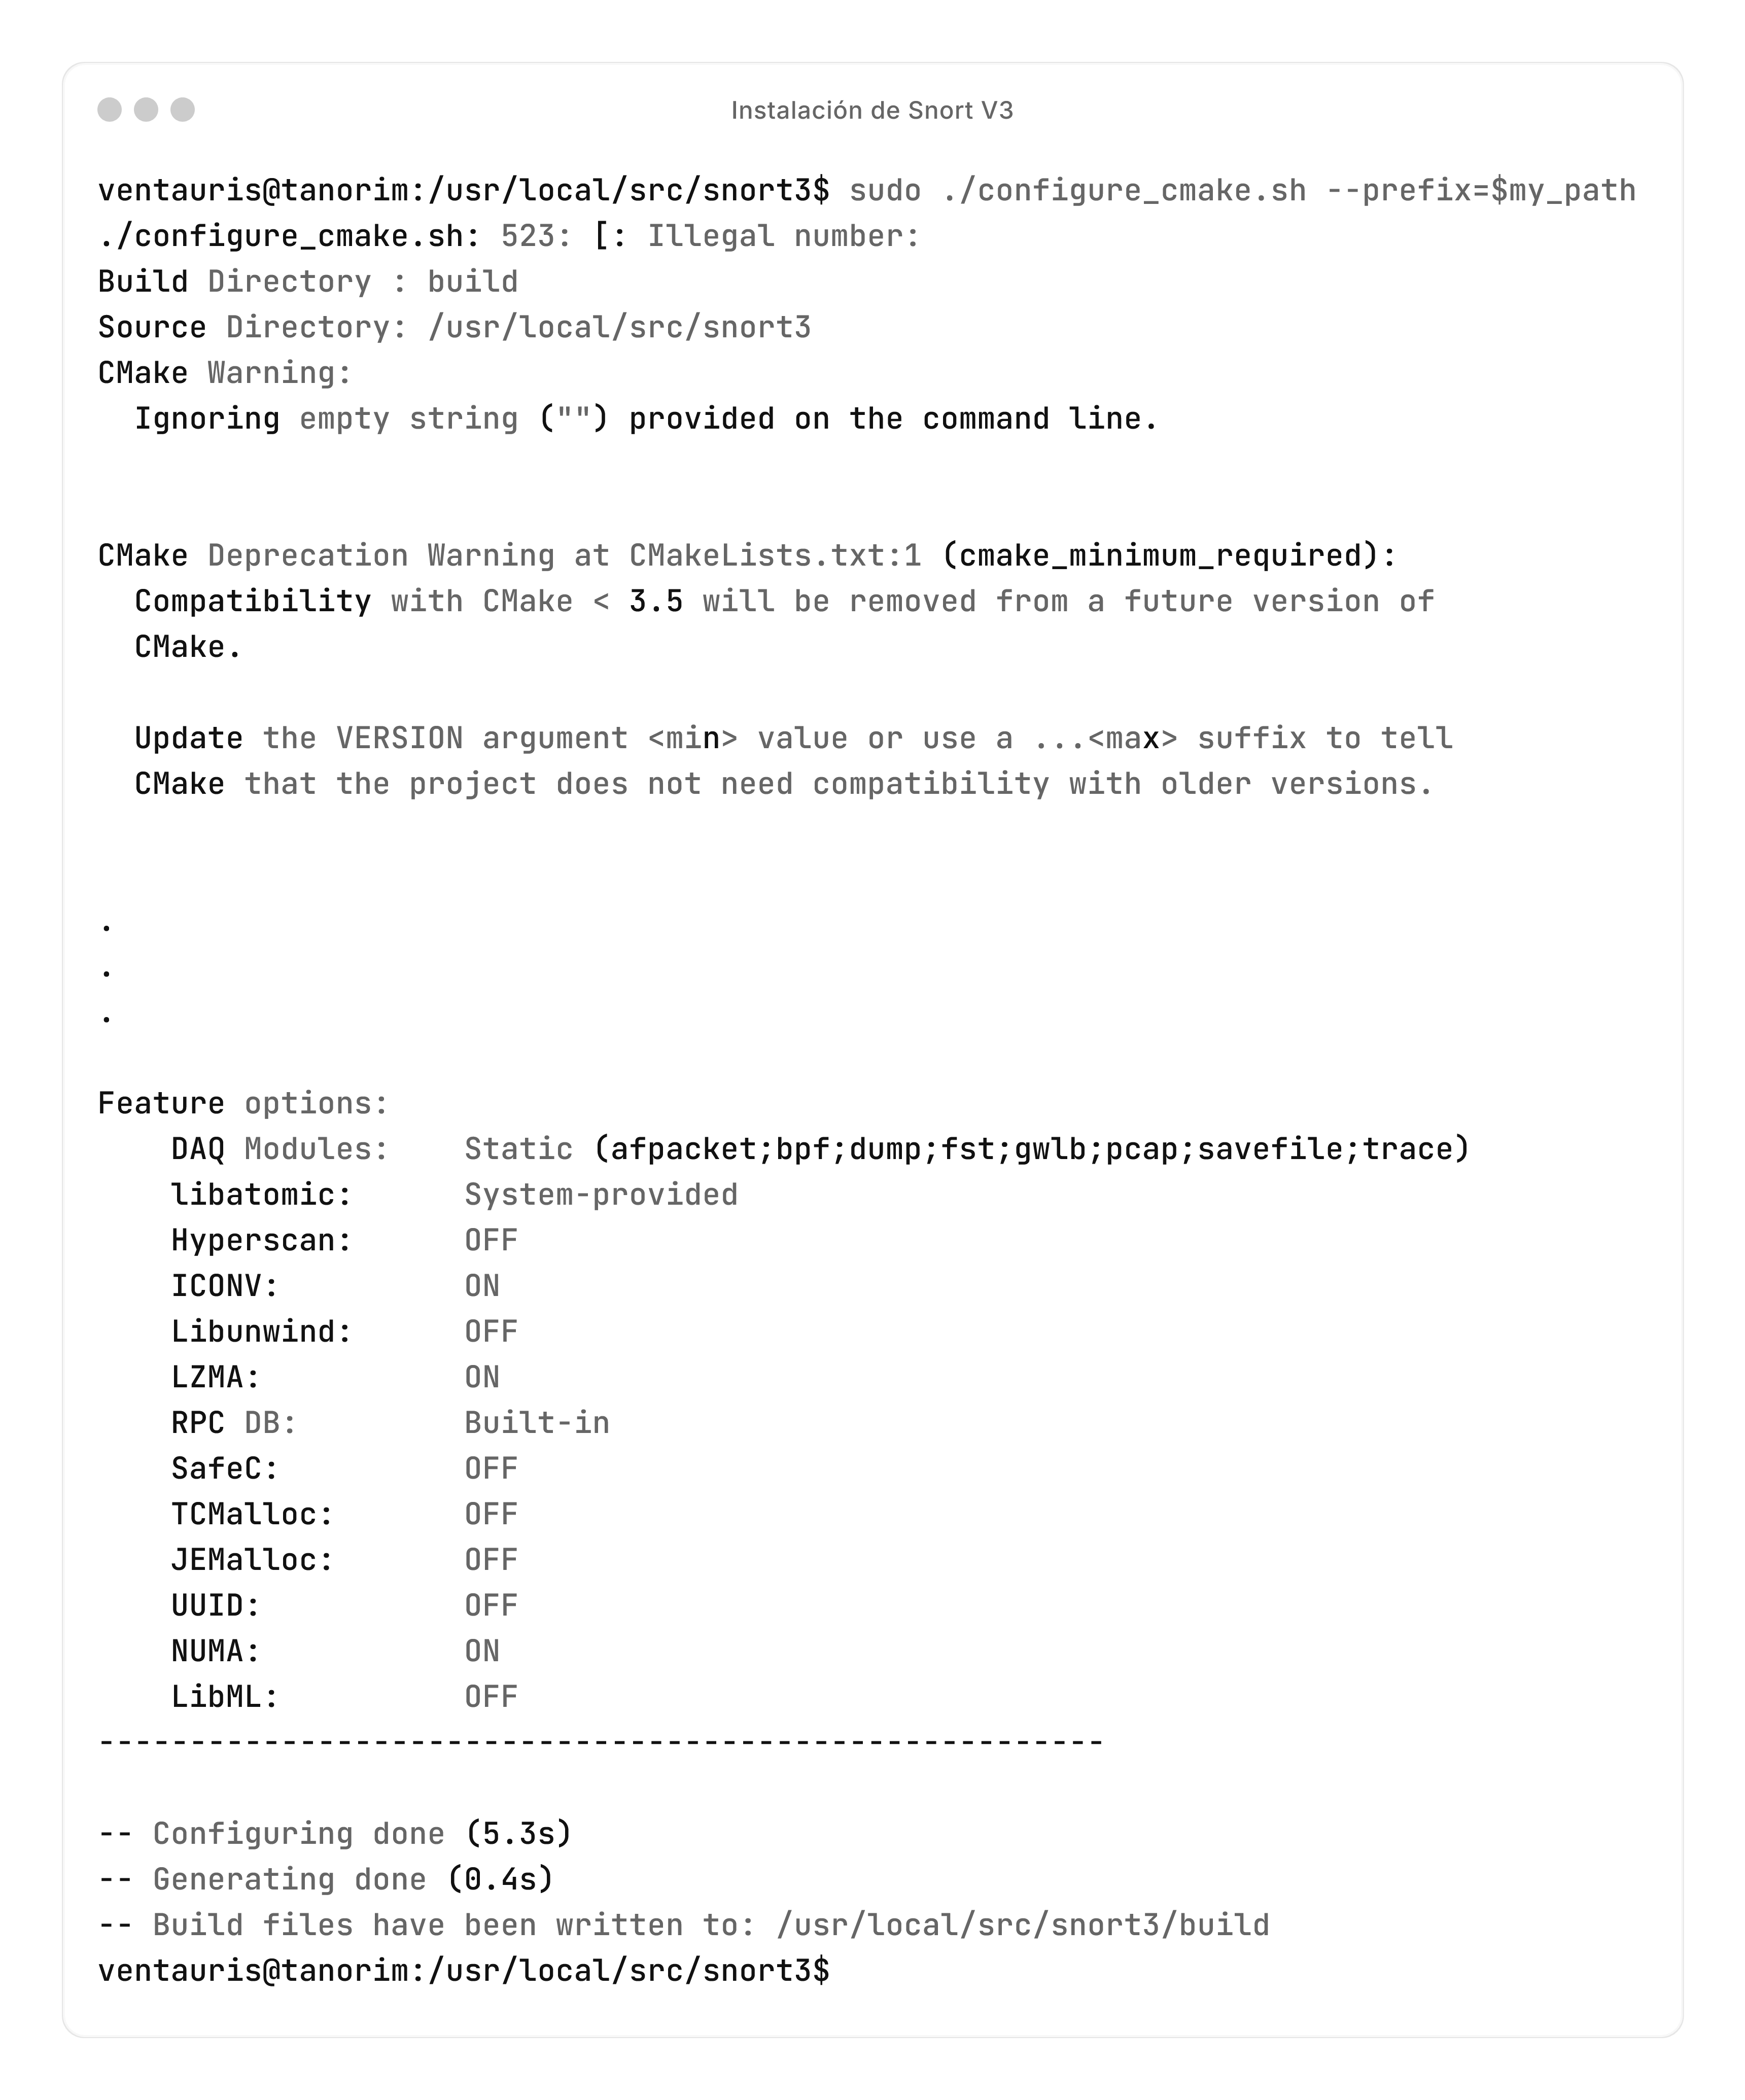
\includegraphics[scale=0.12]{instalacion_snort/21-21.png}
	\caption{Configurando Snort 3 con \texttt{CMake}.}
\end{figure}

\newpage

Compilamos \textbf{Snort} con \texttt{make -j \$(nproc)}, lo que nos permite aprovechar todos los núcleos del procesador para acelerar el proceso.

\begin{figure}[H]
	\centering
	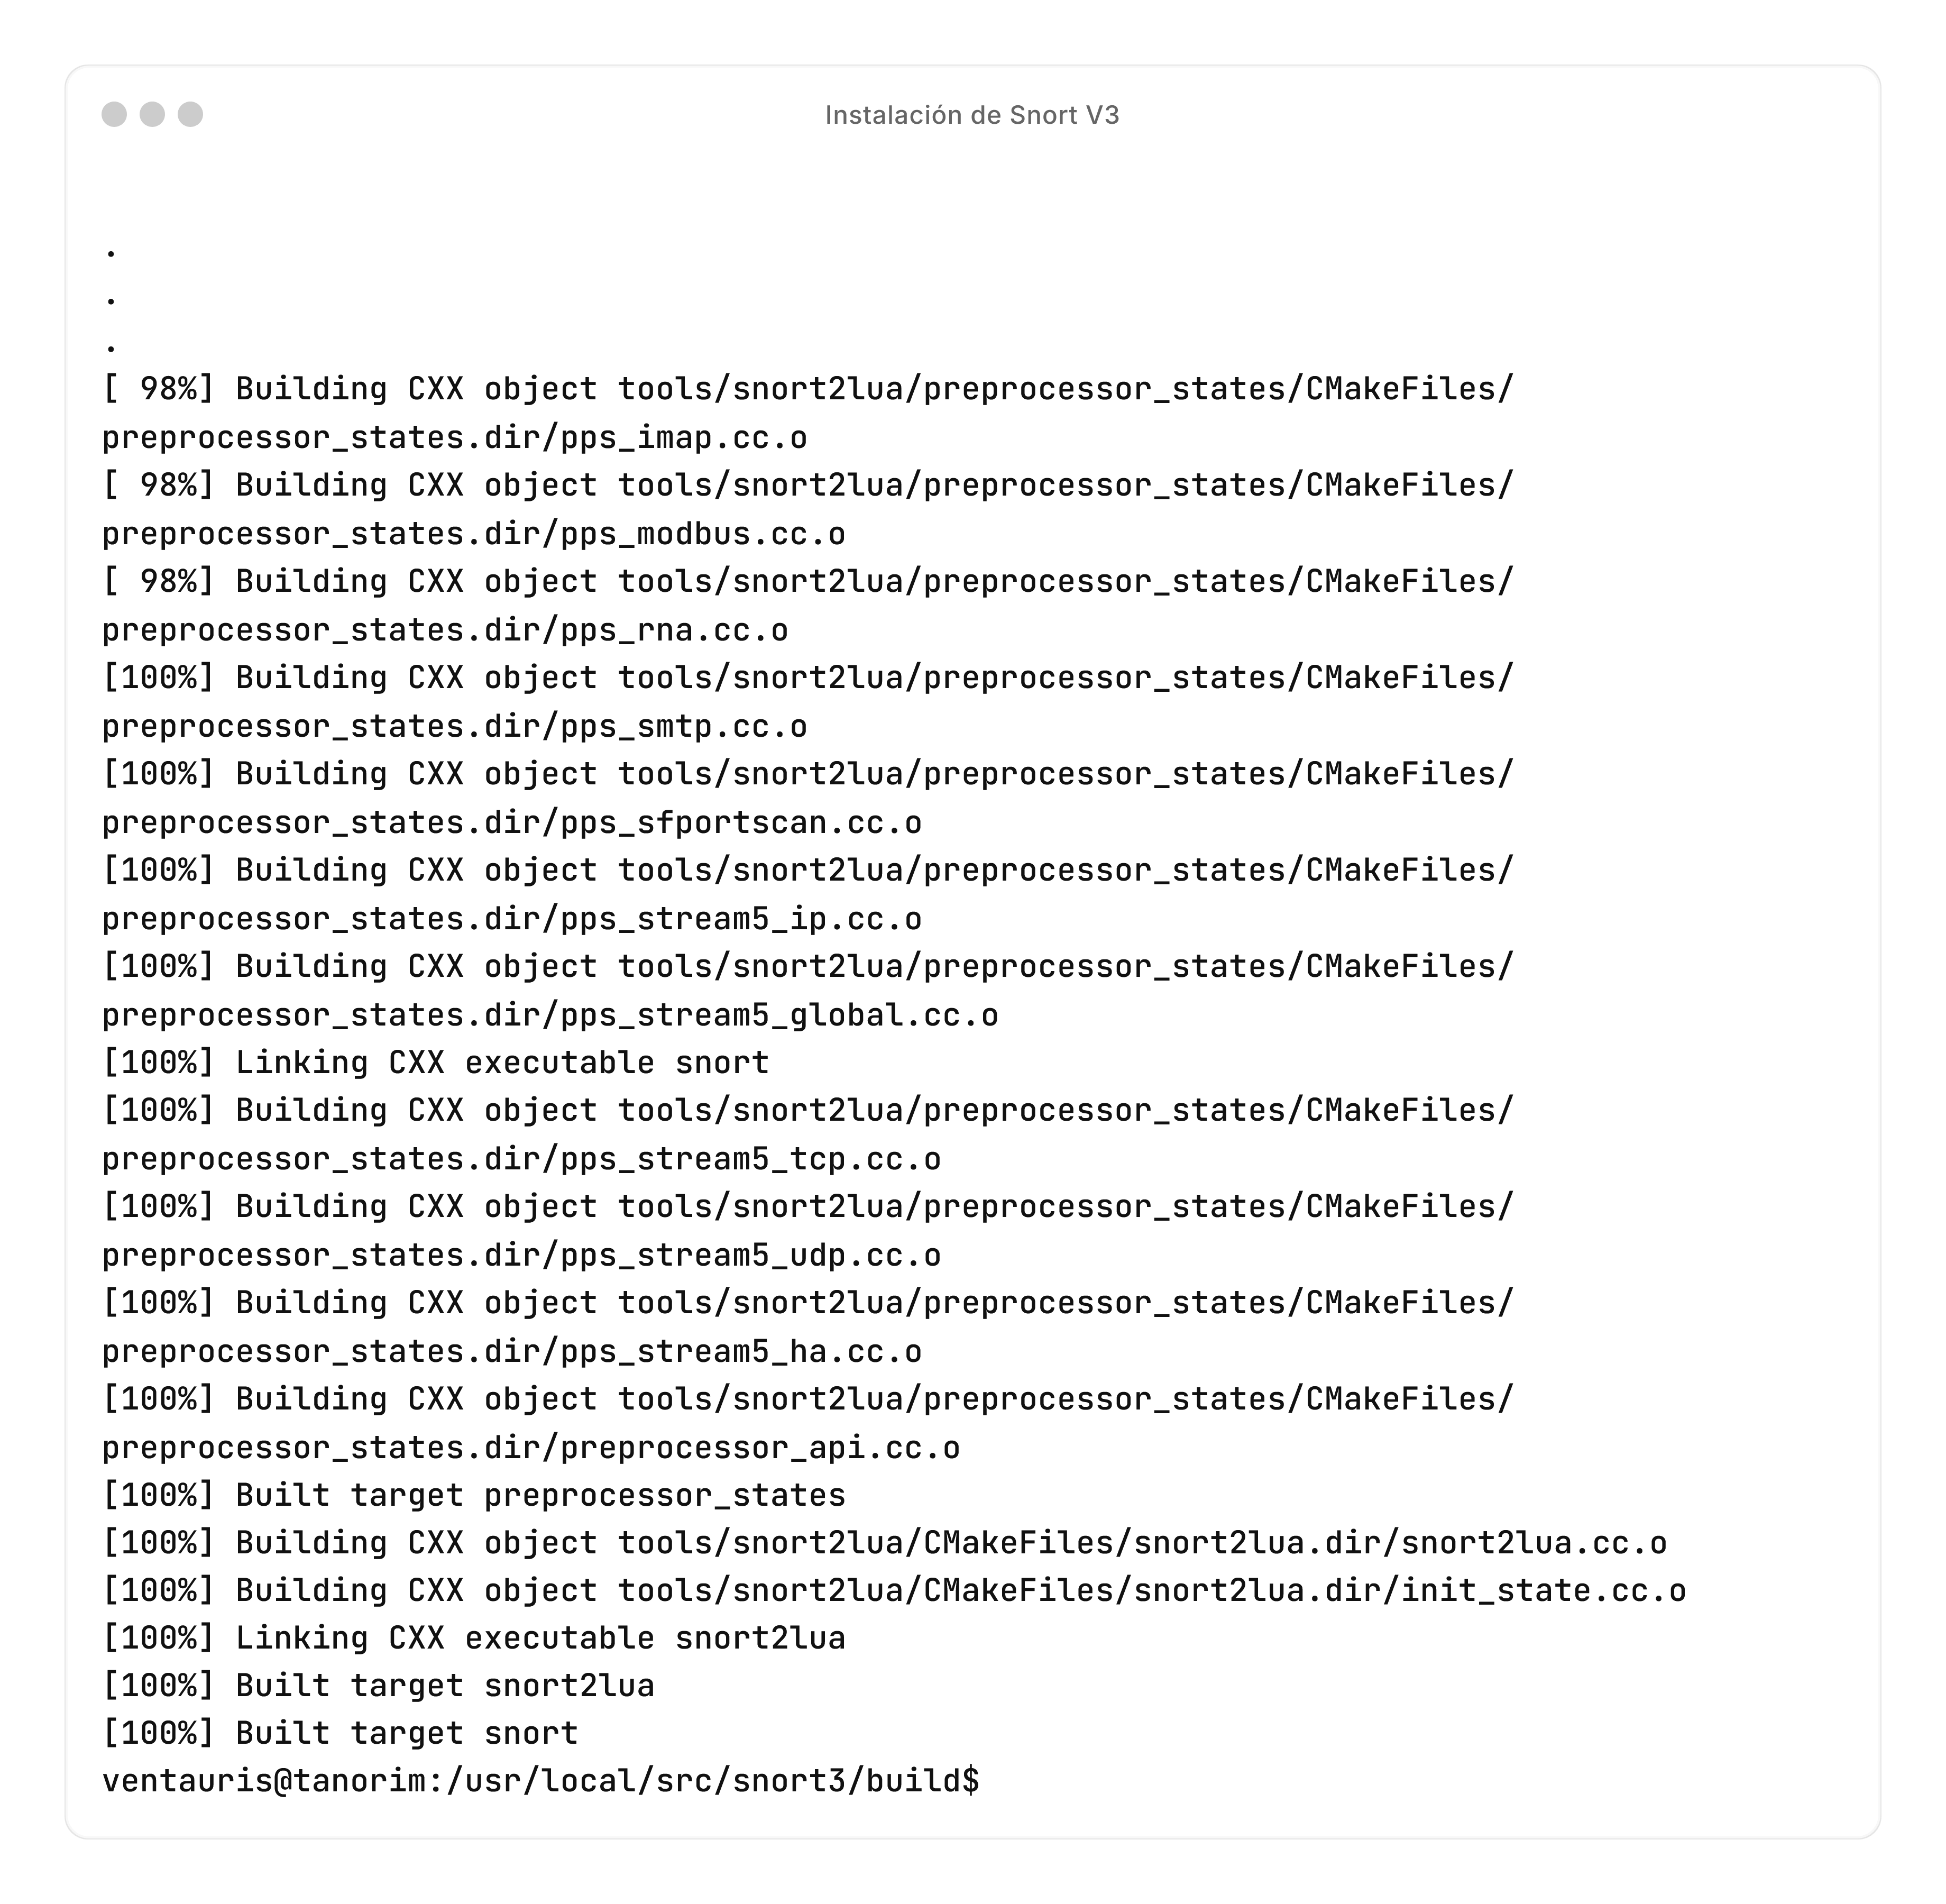
\includegraphics[scale=0.12]{instalacion_snort/22-22.png}
	\caption{Compilación de Snort.}
\end{figure}

\newpage

Instalamos Snort tras haberlo compilado con \texttt{sudo make install}. Este comando copia los archivos generados en sus respectivas ubicaciones dentro del sistema.

\begin{figure}[H]
	\centering
	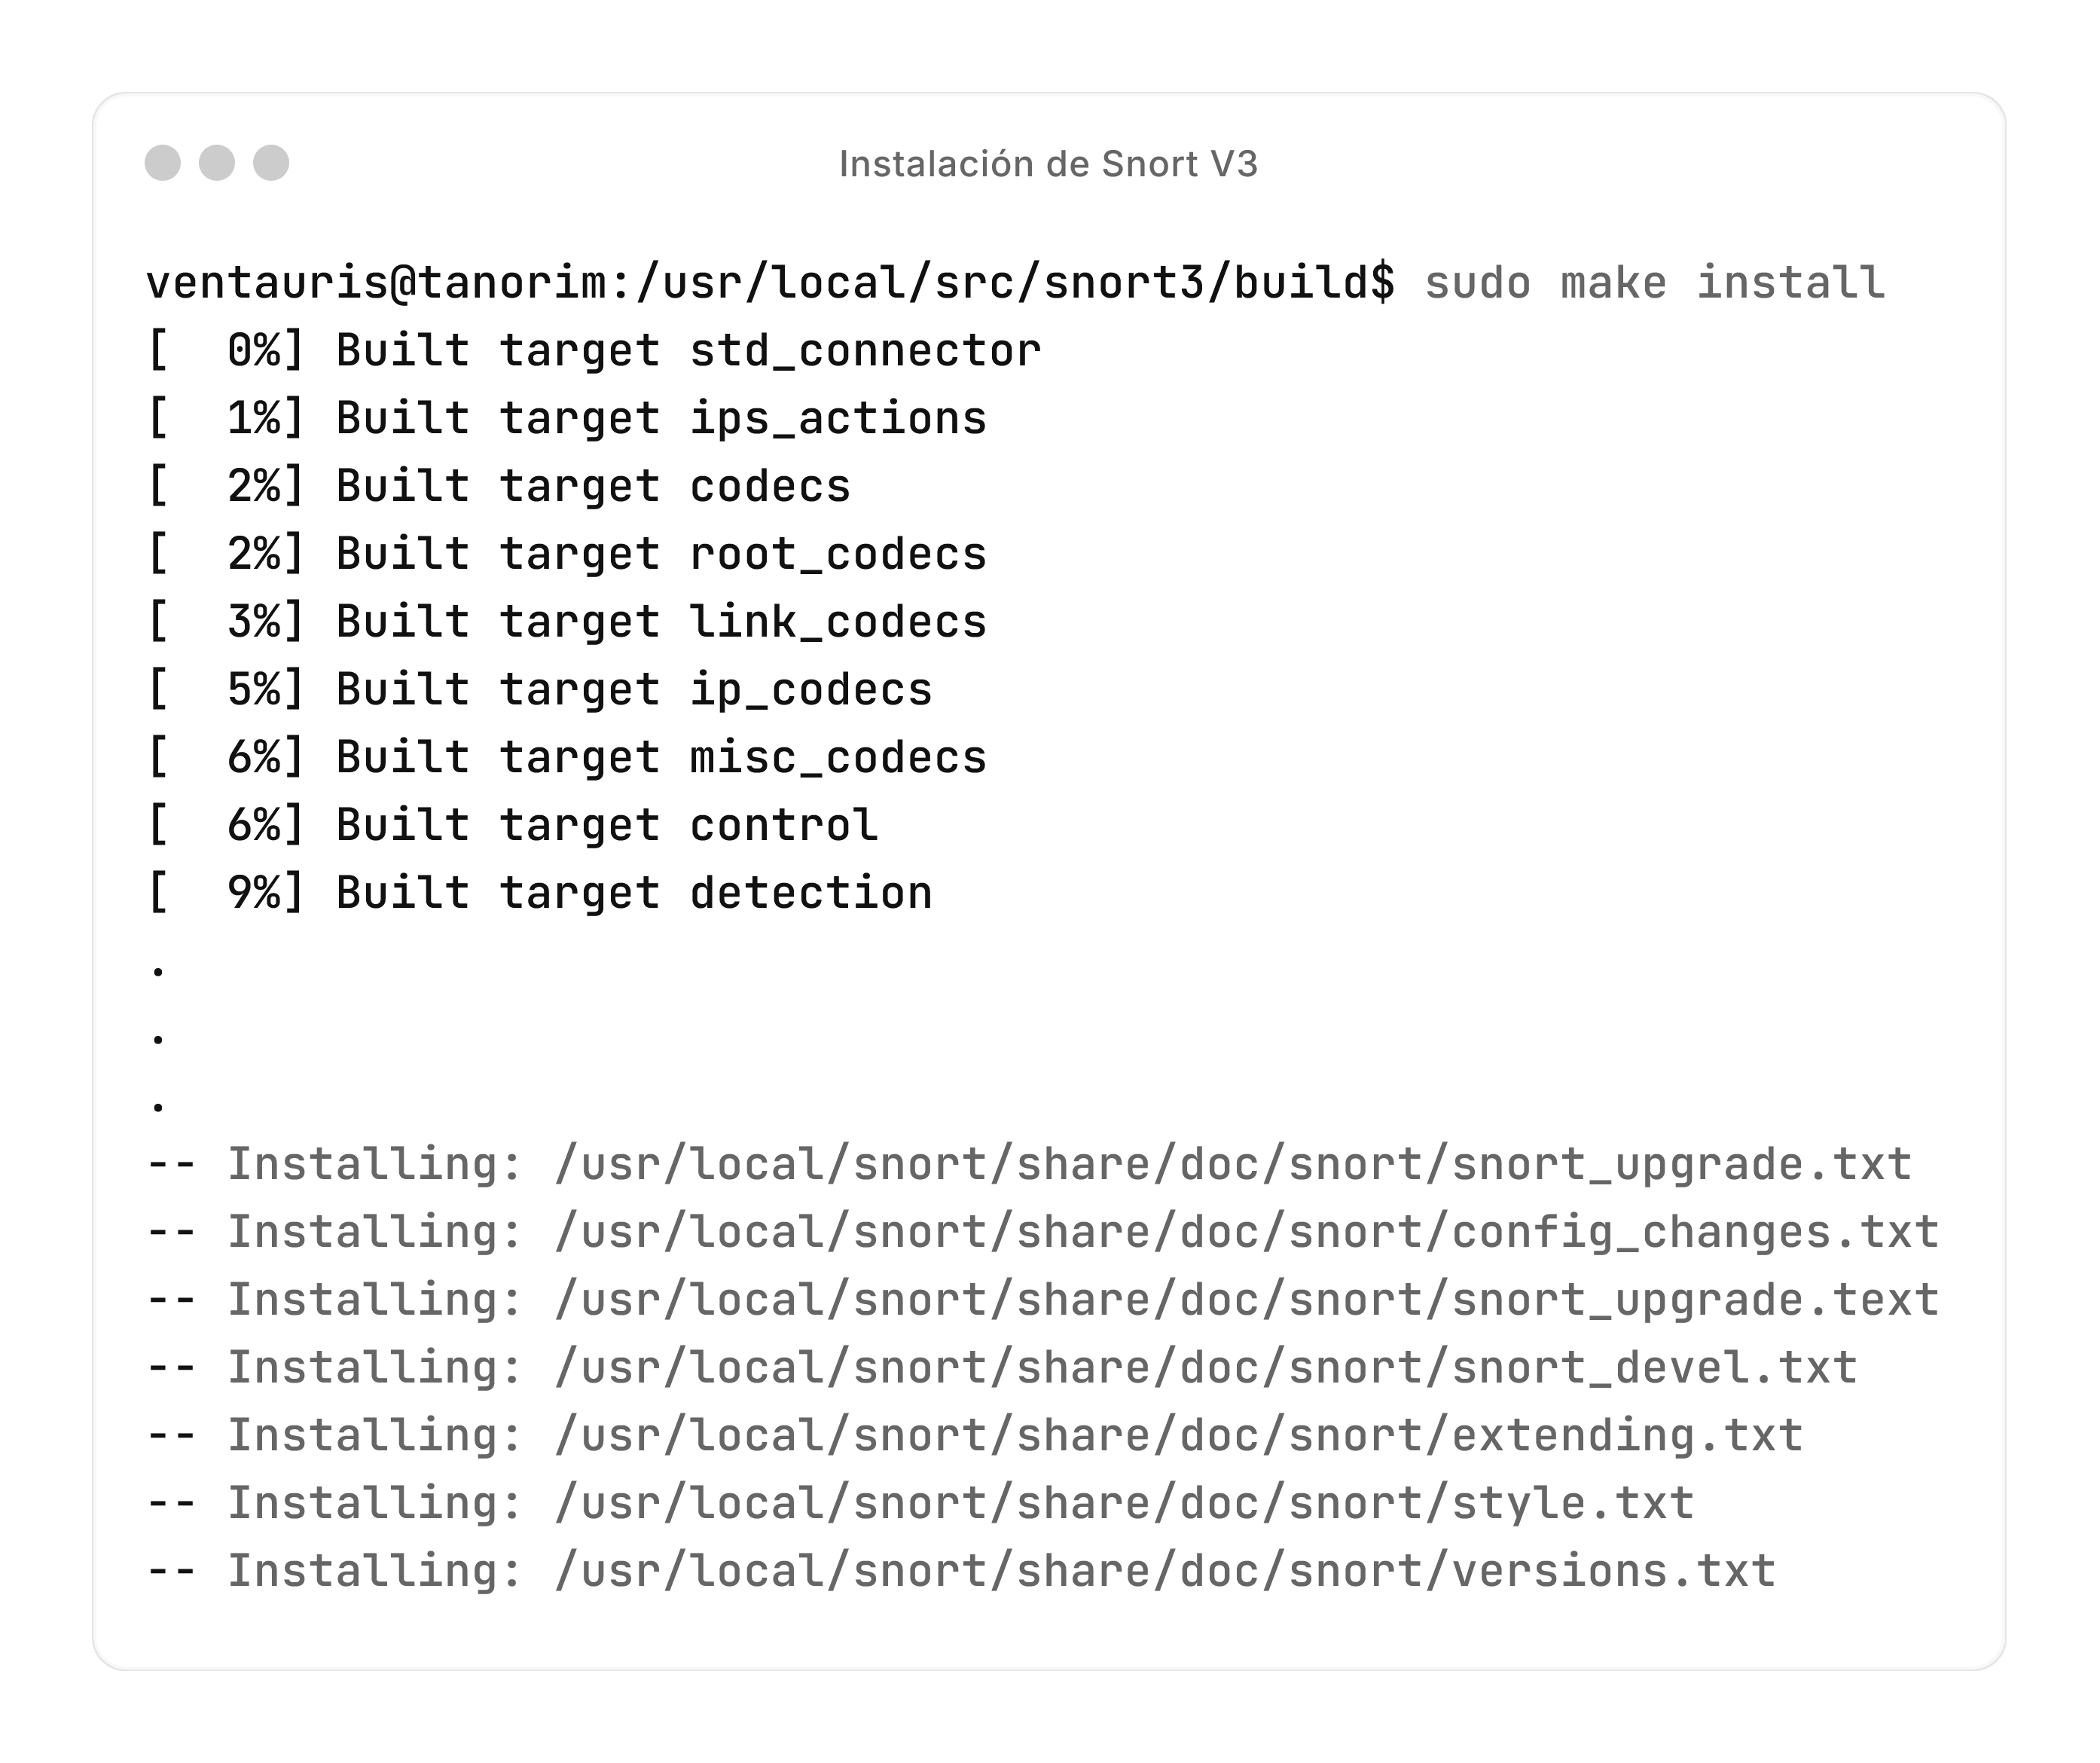
\includegraphics[scale=0.12]{instalacion_snort/23-23.png}
	\caption{Instalación de Snort.}
\end{figure}

Finalmente, verificamos que \textbf{Snort} se ha instalado correctamente con el comando \texttt{/usr/local/snort/bin/snort -V}. Esto nos muestra la versión instalada (\textbf{3.7.1.0}) junto con las bibliotecas y dependencias utilizadas, como \texttt{DAQ}, \texttt{libpcap}, \texttt{LuaJIT}, \texttt{OpenSSL}, entre otras.

\begin{figure}[H]
	\centering
	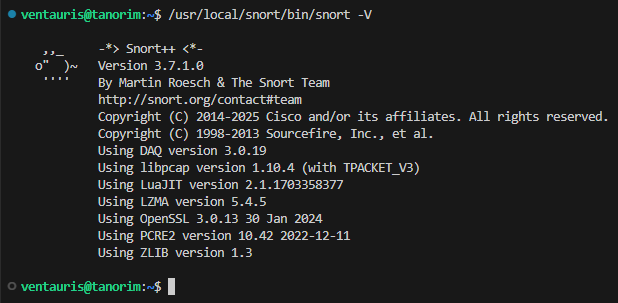
\includegraphics[scale=0.7]{instalacion_snort/24.png}
	\caption{Snort instalado con éxito.}
\end{figure}

\newpage

Creamos el directorio de configuración de Snort (\texttt{/usr/local/snort/etc/snort}) y copiamos los archivos de configuración en formato \texttt{Lua} desde el directorio fuente de \textbf{Snort 3}. Luego, ejecutamos Snort con la configuración especificada para validar que todo esté correctamente configurado. La salida muestra que Snort ha cargado las reglas y módulos sin errores ni advertencias.

\begin{figure}[H]
	\centering
	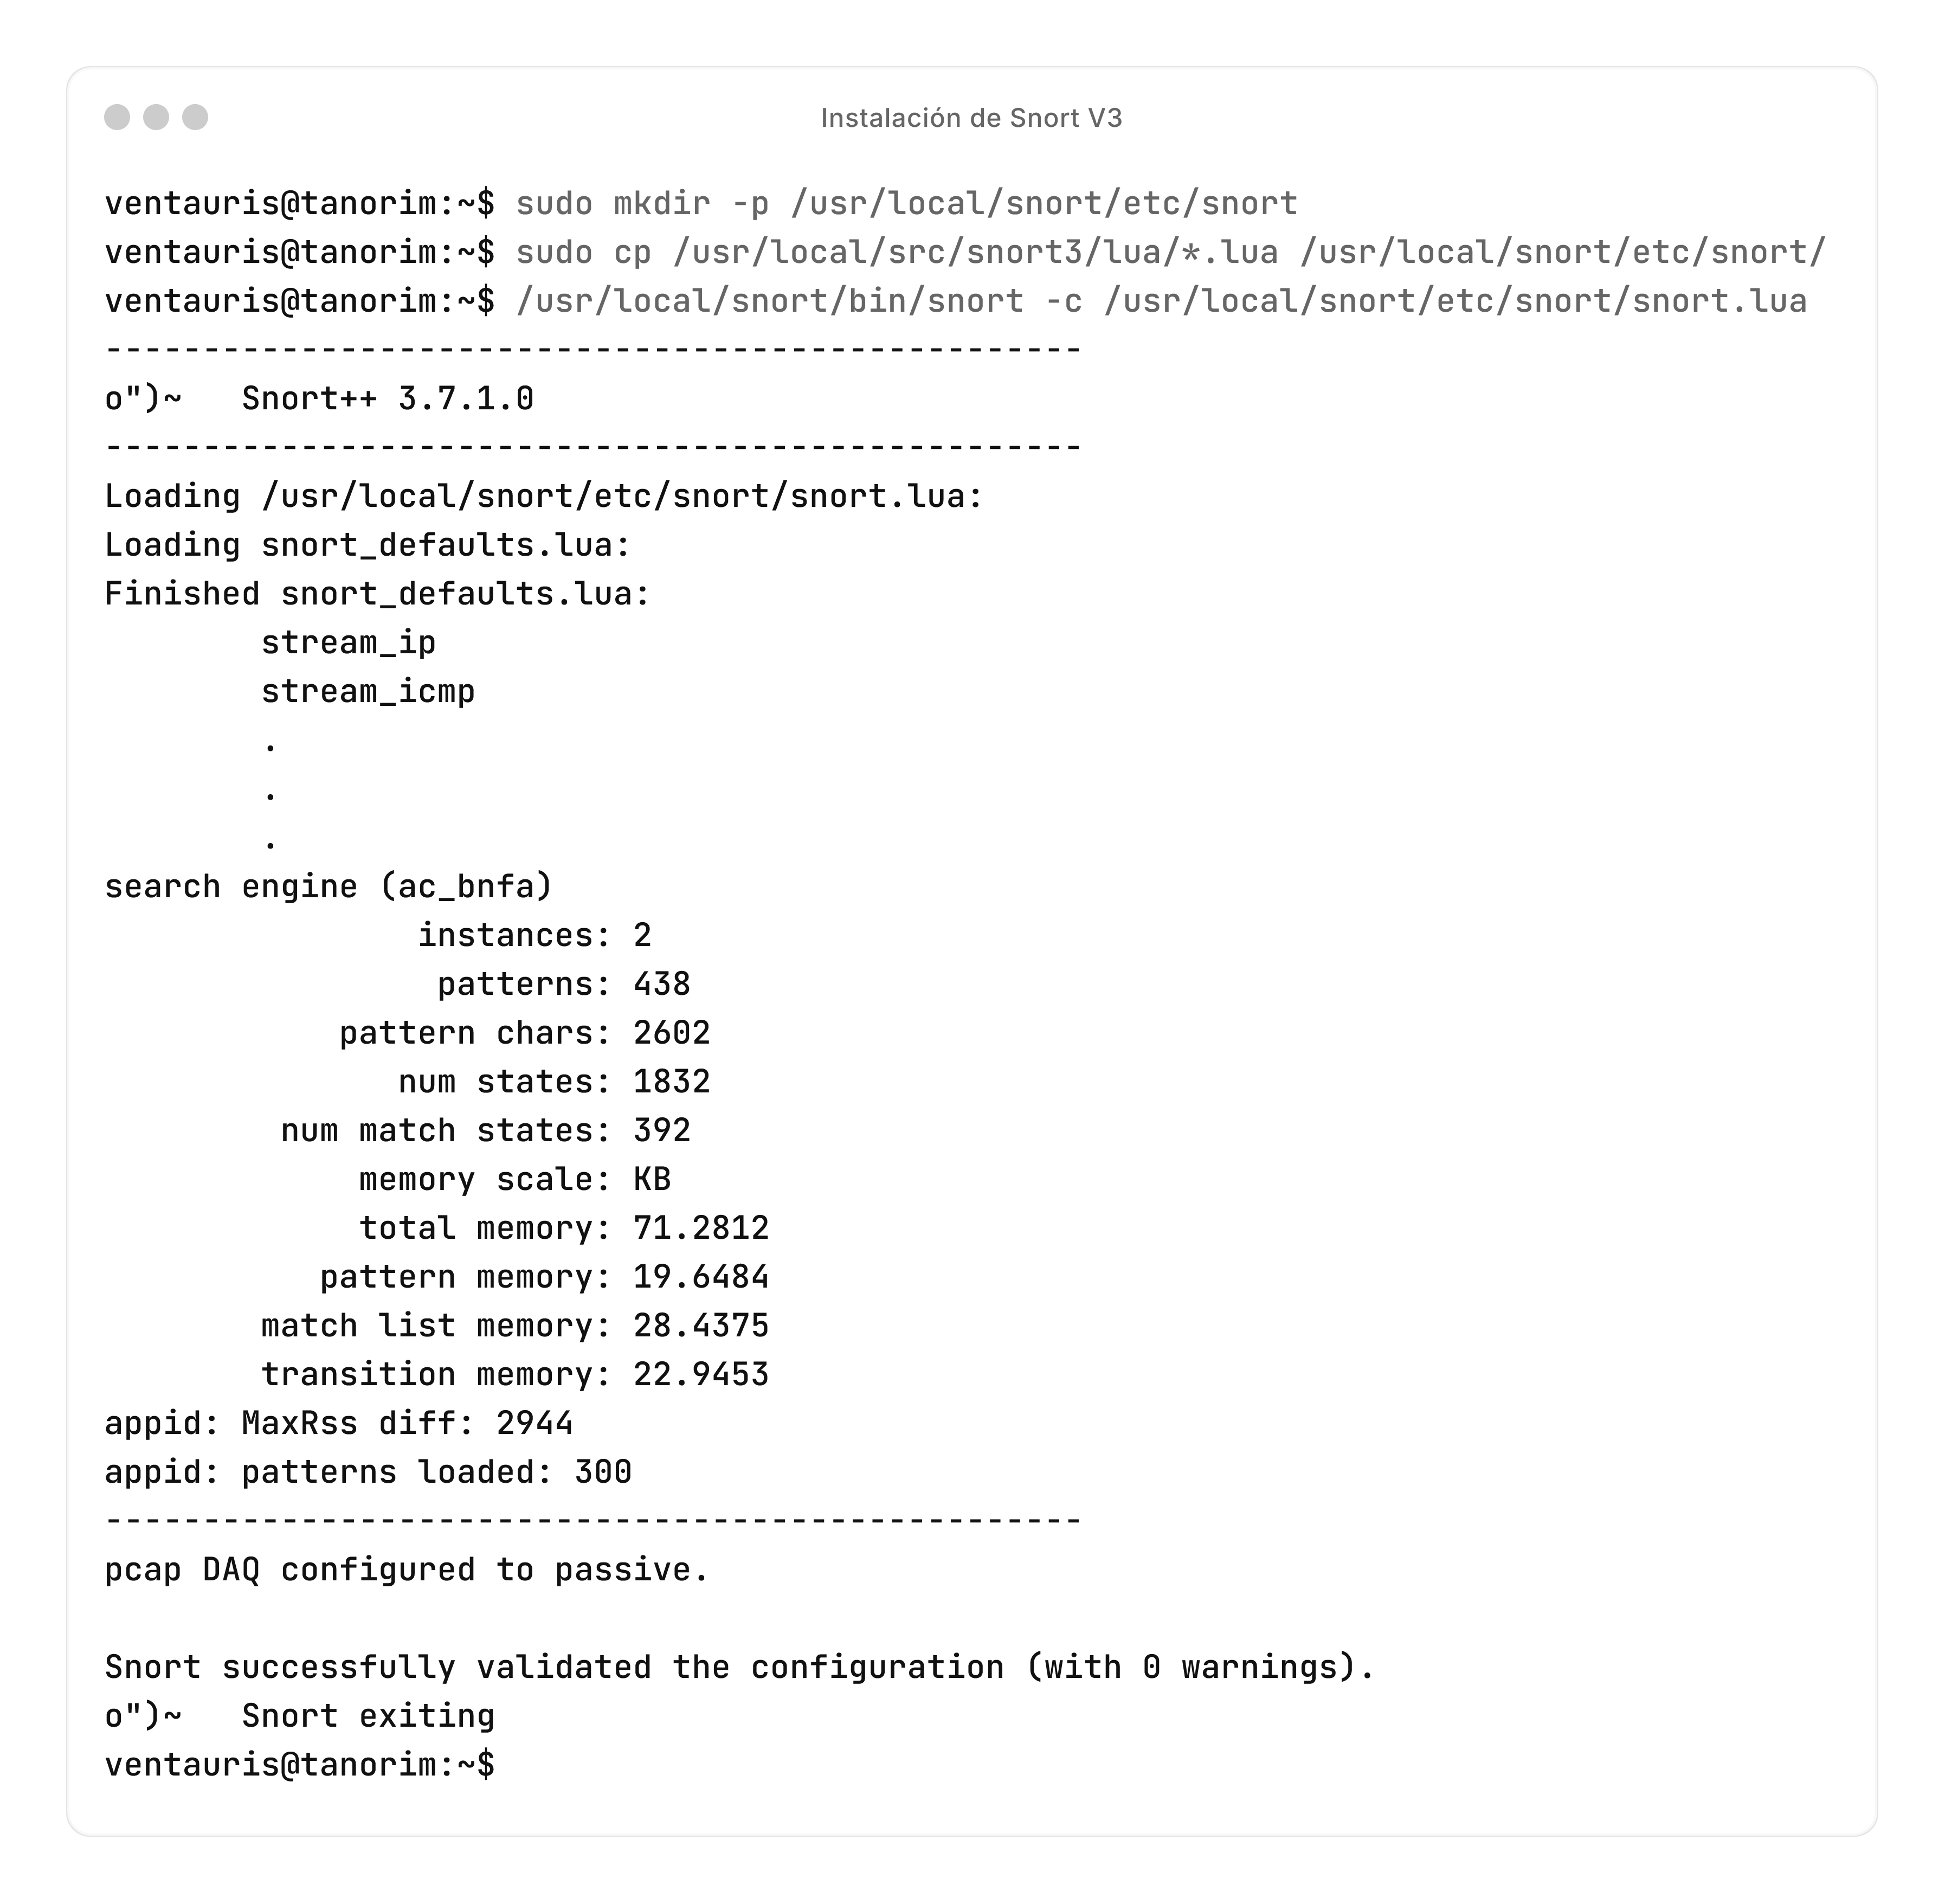
\includegraphics[scale=0.12]{instalacion_snort/25-25.png}
	\caption{Configuración de Snort validada con éxito.}
\end{figure}

%%%%%%%%%%%%%%%%%%%%%%%%%%%%HECHO3

\newpage

\subsection{Instalación de reglas y plugins}

Tras la correcta instalación de \textbf{Snort}, aprovecharemos la arquitectura modular introducida en la versión 3, la cual utiliza archivos con extensión \texttt{.lua} para gestionar su configuración de forma más flexible y estructurada. A continuación, se presenta una guía paso a paso sobre cómo instalar las reglas básicas proporcionadas por la comunidad de Snort, conocidas como \textit{Community Rules}.
\newline

Descargamos las \textit{Community Rules} de Snort utilizando el comando \texttt{wget}, seguido de su descompresión mediante \texttt{tar}. Estas reglas constituyen un conjunto de firmas predefinidas para detectar amenazas comunes en entornos de red.

\begin{figure}[H]
	\centering
	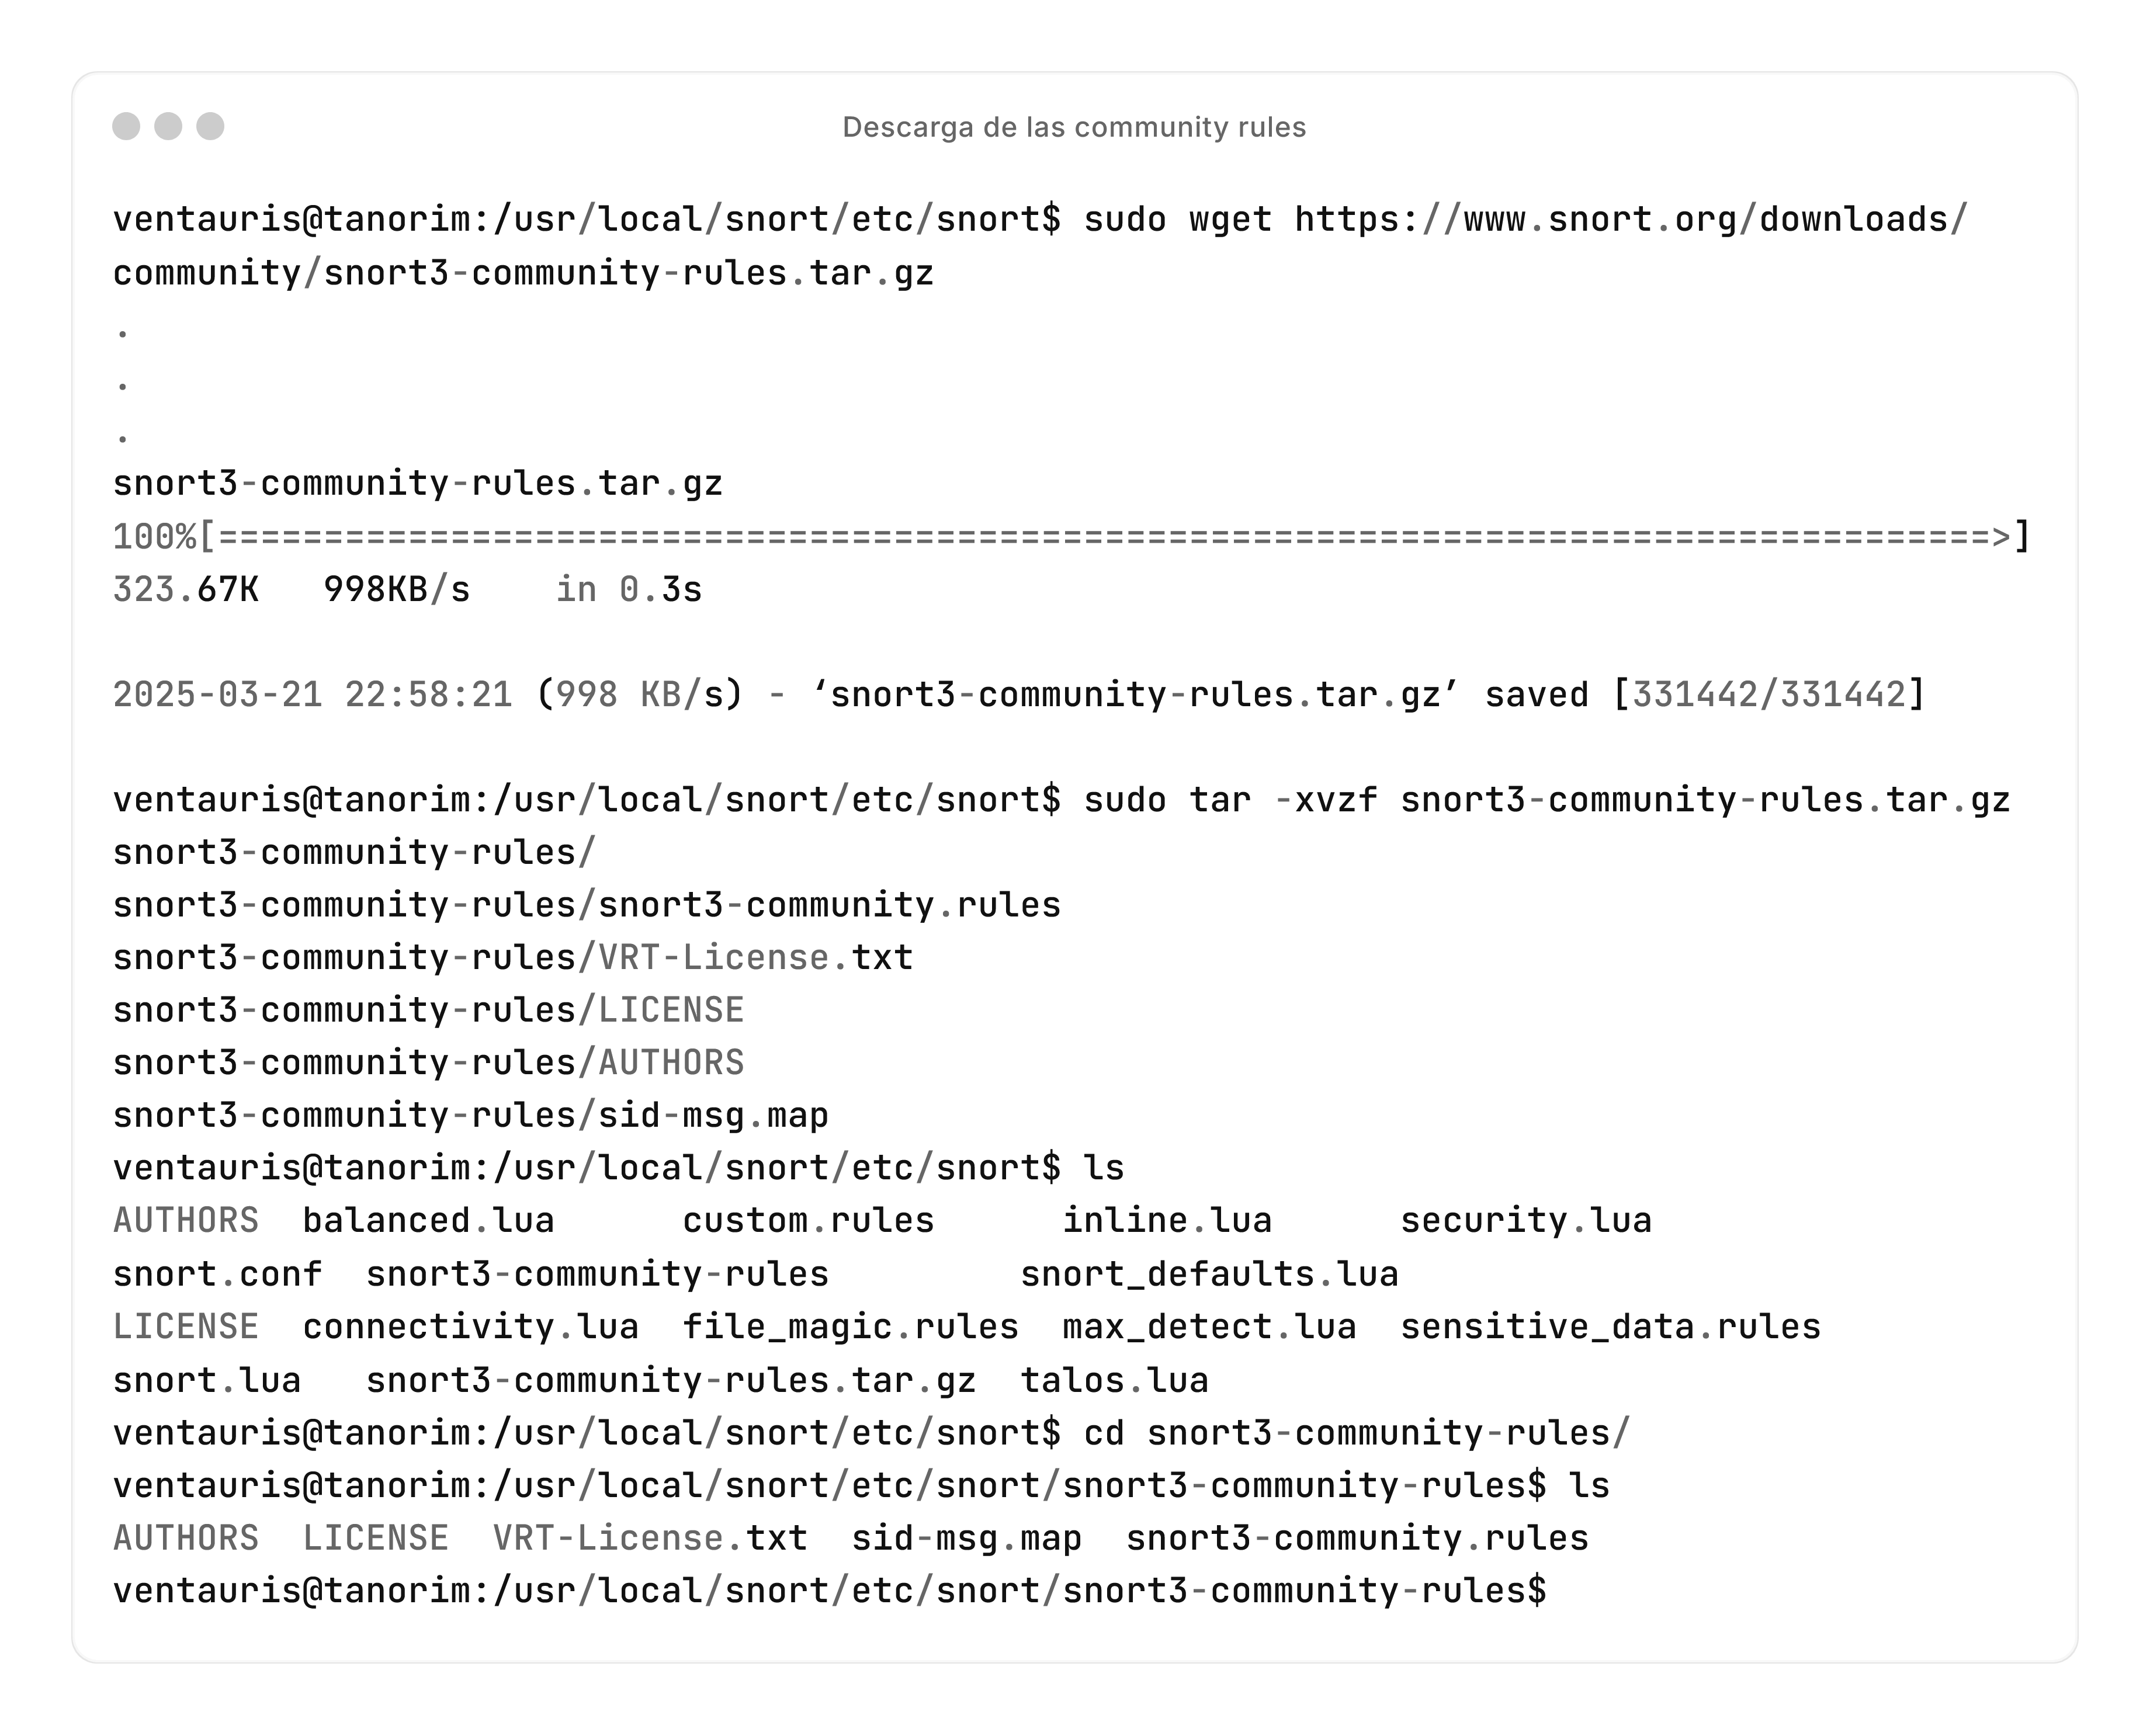
\includegraphics[scale=0.12]{instalacion_reglas_snort/1-1.png}
	\caption{Añadiendo reglas preconfiguradas a Snort.}
\end{figure}

\pagebreak

Posteriormente, editamos el archivo \texttt{snort.lua}, ubicado en \texttt{/usr/local/snort/etc/snort/}, para incluir la ruta del archivo \texttt{community.rules}. Esto permite que Snort cargue automáticamente estas reglas al iniciar y pueda utilizarlas para detectar patrones maliciosos en el tráfico de red. La edición del archivo puede realizarse con herramientas como \texttt{nano}, \texttt{vim} o cualquier otro editor de texto de preferencia.

\begin{figure}[H]
	\centering
	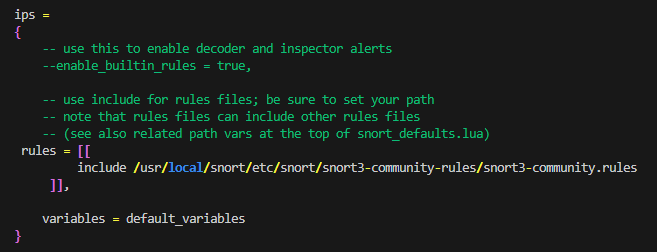
\includegraphics[scale=0.8]{instalacion_reglas_snort/2.png}
	\caption{Modificación de \texttt{snort.lua} para agregar las reglas preconfiguradas.}
\end{figure}

Una vez agregadas las reglas a \texttt{snort.lua}, realizamos una validación de la configuración ejecutando Snort en modo prueba. Esto permite comprobar que no existan errores sintácticos o de carga, garantizando así que el sistema pueda funcionar correctamente.

\begin{figure}[H]
	\centering
	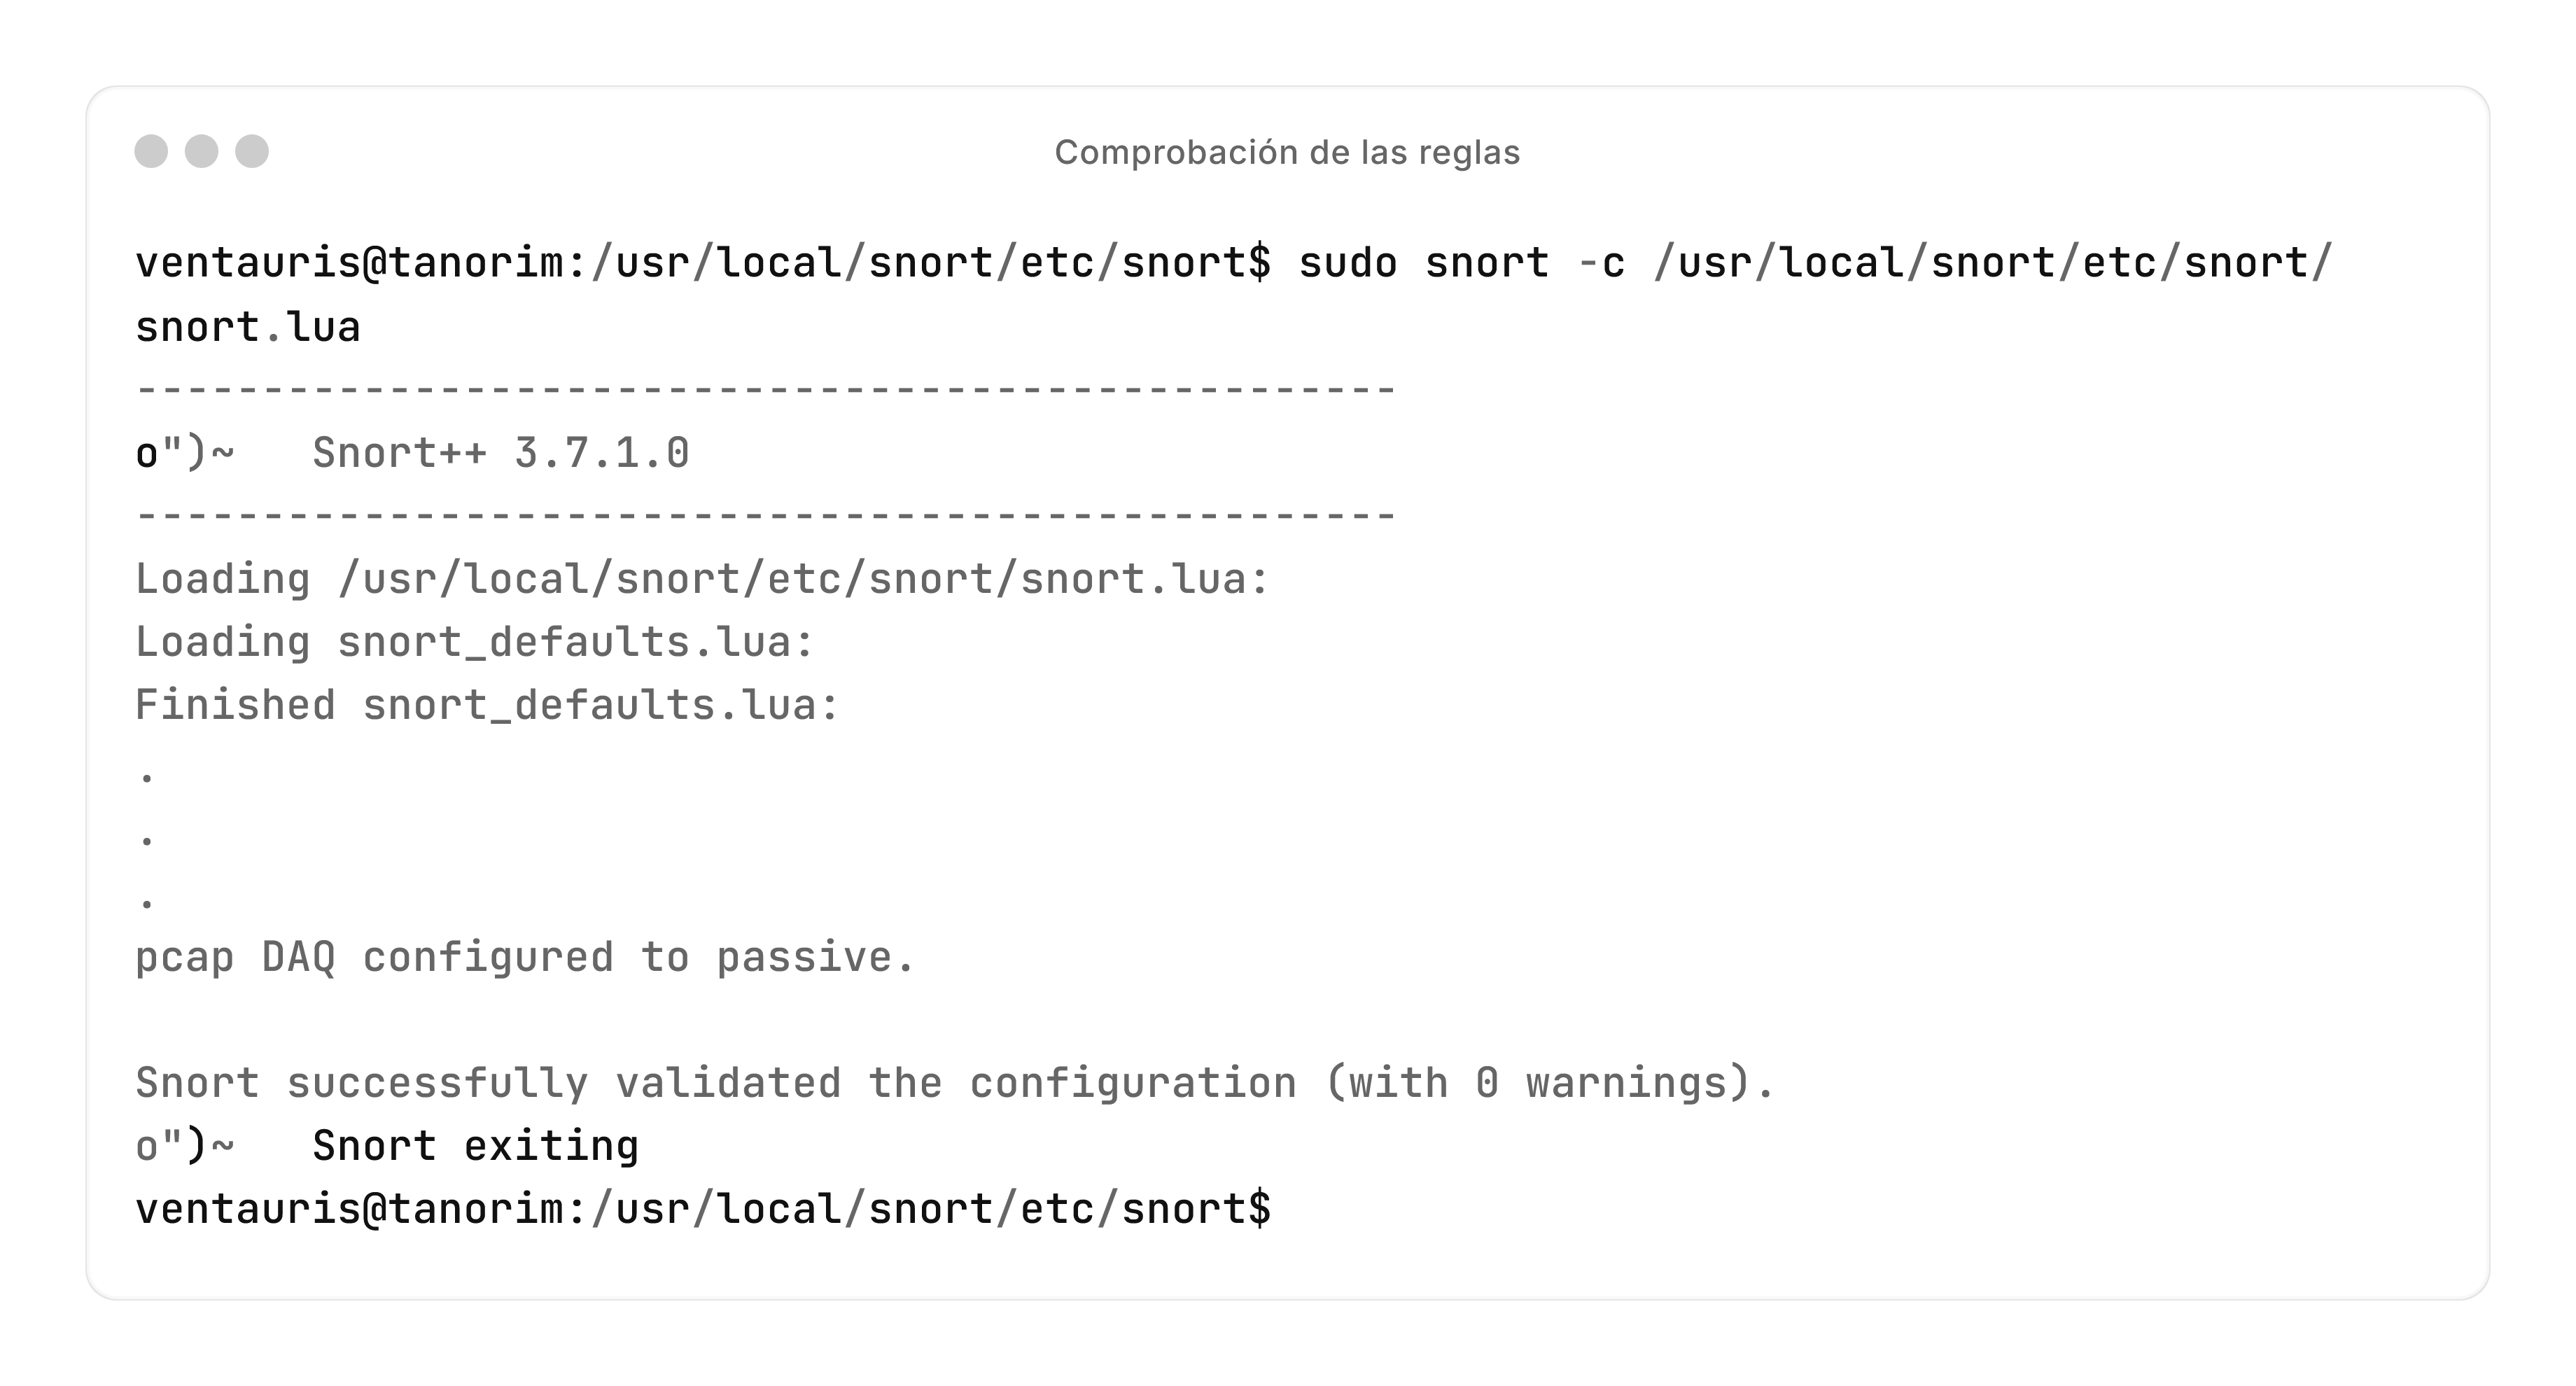
\includegraphics[scale=0.12]{instalacion_reglas_snort/3-3.png}
	\caption{Validación configuración de Snort.}
\end{figure}

\newpage

\subsection{Configuración preprocesador HTTP Inspect}

Accedemos al archivo \texttt{snort.lua} y localizamos la sección correspondiente al preprocesador \texttt{http\_inspect = \{\}}. En ella escribimos los parámetros adecuados para la gestión y protección de una red corporativa de pequeña o mediana empresa (PYME). Esta configuración permite a Snort analizar a fondo el tráfico HTTP y detectar comportamientos anómalos asociados a amenazas comunes como ataques por inyección, carga de malware o manipulación de cabeceras.

Las reglas aplicadas son las siguientes:
\newline

\begin{table}[ht]
	\centering
	\begin{tabular}{l l p{7cm}}
		\hline
		\textbf{Parámetro} & \textbf{Valor} & \textbf{Uso en una PYME}\\
		\hline
		\texttt{request\_depth}       & \texttt{-1} & Inspeccionar todo el contenido de la petición HTTP. Permite detectar inyecciones SQL, código malicioso y malware embebido.\\
		\texttt{response\_depth}      & \texttt{-1} & Revisar la totalidad de la respuesta enviada por el servidor, útil para detectar descargas de archivos maliciosos.\\
		\texttt{unzip}                & \texttt{true} & Habilita la descompresión de contenidos codificados como gzip o deflate. Evita que el contenido malicioso comprimido pase desapercibido.\\
		\texttt{oversize\_dir\_length}& \texttt{500} & Genera alertas si una URI presenta una ruta anormalmente larga, característica común en ataques de desbordamiento o evasión.\\
		\texttt{maximum\_headers}     & \texttt{200} & Detecta un número excesivo de cabeceras HTTP, que puede ser indicio de ataques por manipulación de protocolo.\\
		\hline
	\end{tabular}
	\caption{Parámetros de \texttt{http\_inspect}.}
\end{table}

\begin{figure}[H]
	\centering
	\begin{minipage}[b]{0.45\textwidth}
		\centering
		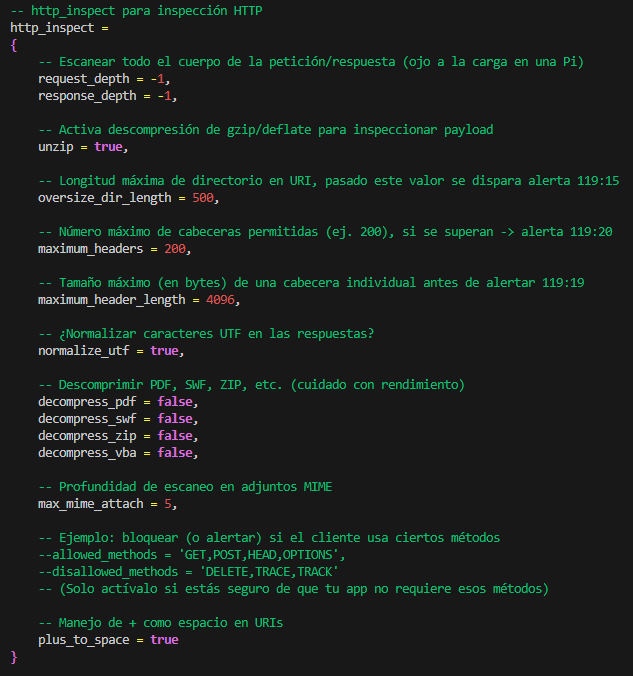
\includegraphics[scale=0.4]{http_inspect/4.png}
		\caption{Configuración \texttt{http\_inspect}.}
	\end{minipage}
	\hfill
	\begin{minipage}[b]{0.45\textwidth}
		\centering
		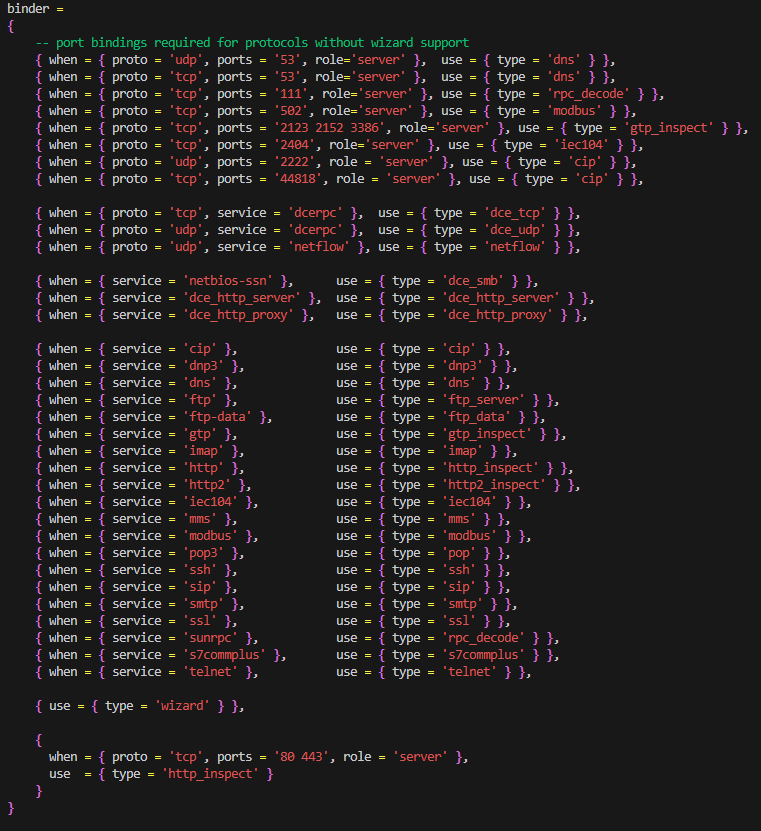
\includegraphics[scale=0.35]{http_inspect/5.png}
		\caption{Configuración de \texttt{binders}.}
	\end{minipage}
\end{figure}

%%%%%%%%%%%%%%%%%%HECHO4

Además de la configuración general de \texttt{http\_inspect} mostrada en la Figura 6.30, es necesario agregar, al final de la sección de \texttt{binders} en el archivo \texttt{snort.lua}, el bloque de código representado en la Figura 6.31 para asegurar su correcto funcionamiento.
\newline

Esta configuración adicional es esencial para que \textbf{Snort} pueda vincular correctamente el tráfico HTTP con su correspondiente módulo de inspección durante el análisis en tiempo real. Sin este paso, es posible que el motor de detección no aplique correctamente las reglas diseñadas para HTTP, reduciendo así la eficacia del sistema de detección de intrusiones.
\newline

Por último, validamos la configuración ejecutando Snort en modo prueba para asegurarnos de que no se han introducido errores y que todas las configuraciones han sido cargadas exitosamente.

\begin{figure}[H]
	\centering
	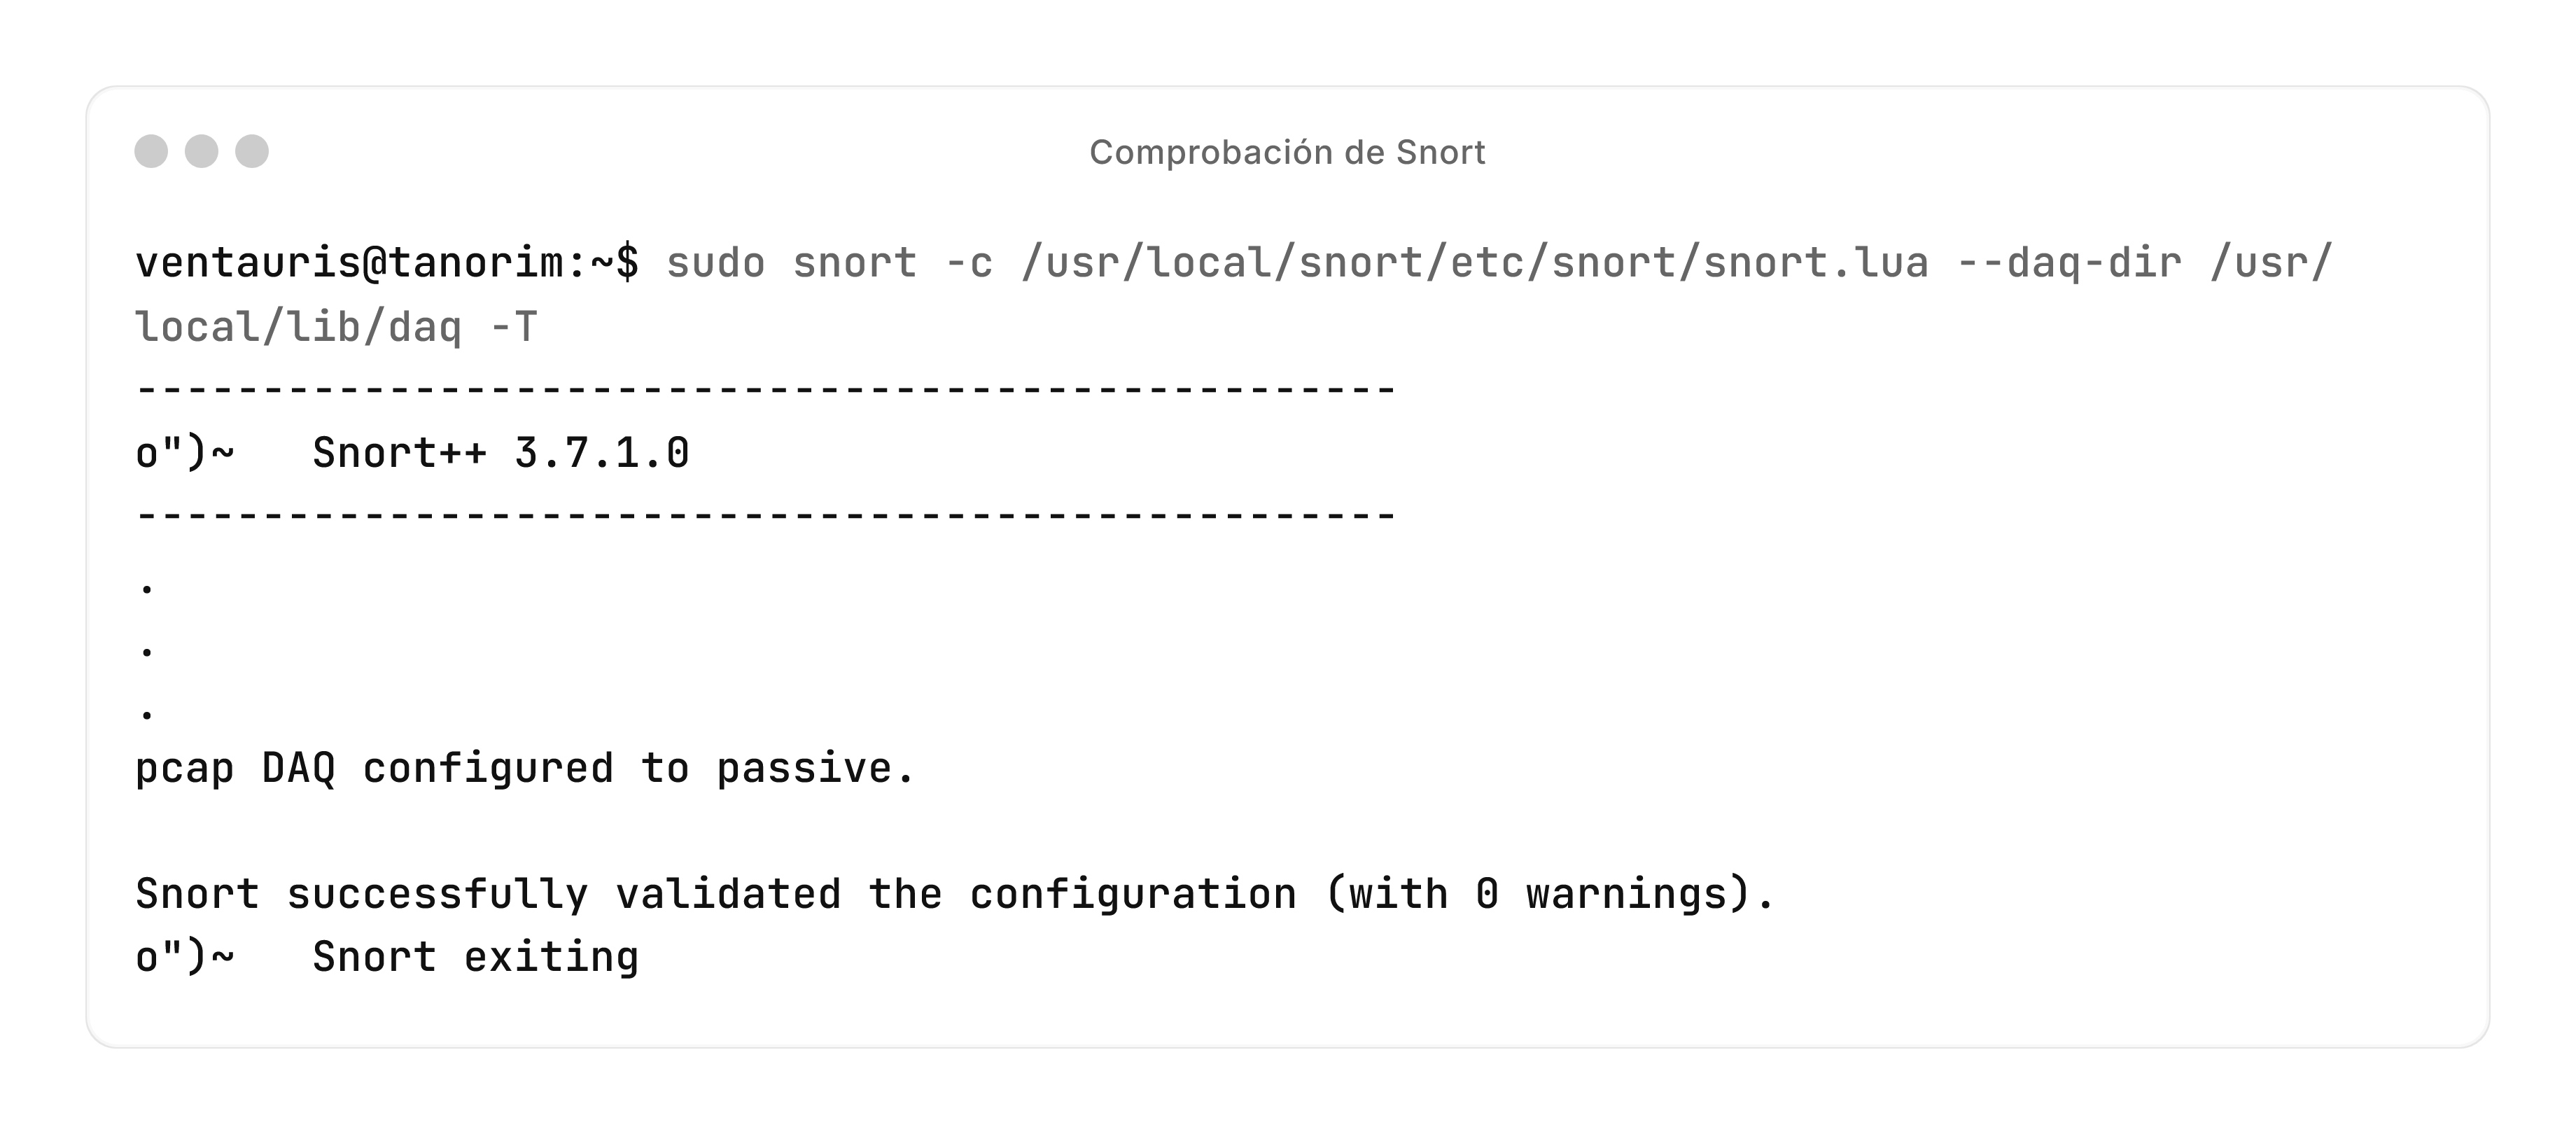
\includegraphics[scale=0.1]{http_inspect/6-6.png}
	\caption{Validación de la configuración.}
\end{figure}


\subsection{SSL Inspector}

El siguiente módulo que habilitaremos será el \textbf{SSL Inspector}. El procedimiento de activación es similar al seguido en módulos anteriores. Comenzaremos por modificar el archivo \texttt{snort.lua}, donde localizaremos la sección correspondiente a \texttt{ssl} y añadiremos el bloque de configuración mostrado a continuación.

\begin{figure}[H]
	\centering
	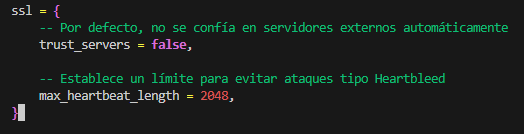
\includegraphics[scale=0.8]{ssl_inspect/8.png}
	\caption{Configuración de SSL.}
\end{figure}

Posteriormente, es necesario vincular la configuración de \texttt{ssl} en la sección \texttt{binders}, en caso de que no se haya hecho previamente. Esta vinculación garantiza que el tráfico cifrado sea correctamente dirigido al módulo de inspección SSL.

\begin{figure}[H]
	\centering
	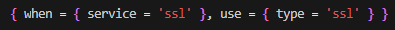
\includegraphics[scale=0.8]{ssl_inspect/9.png}
	\caption{Vincular con \texttt{binders}.}
\end{figure}

A continuación, verificamos la configuración de Snort para asegurarnos de que la sintaxis sea válida. Si todo es correcto, reiniciamos el servicio mediante \texttt{systemctl} para aplicar los cambios.

\subsection{Stream IP}

Antiguamente conocido como \texttt{Frag3}, este preprocesador ha sido reemplazado por una versión más moderna bajo el nombre de \textbf{Stream IP}. Este módulo es responsable de reensamblar fragmentos de paquetes IP para prevenir técnicas de evasión. Su configuración se realiza en el archivo \texttt{snort.lua}.

\begin{figure}[H]
	\centering
	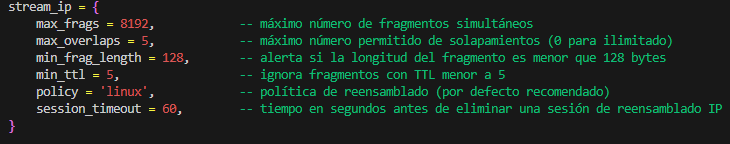
\includegraphics[scale=0.8]{stream_ip/1.png}
	\caption{Configuración de Stream IP.}
\end{figure}

Una vez completada la configuración, validamos la sintaxis del archivo y reiniciamos Snort para aplicar los cambios.

\newpage

\subsection{Stream TCP}

Otro preprocesador que puede marcar la diferencia en protección de redes SOHO es \textbf{Stream TCP}, sucesor de \texttt{Stream5}. Este módulo permite el reensamblado de flujos TCP, lo cual es esencial para una inspección precisa del tráfico de red a nivel de sesión. Su configuración se realiza de forma similar a \texttt{Stream IP}. Tras editar \texttt{snort.lua}, comprobamos la validez de la sintaxis y reiniciamos el servicio.

\begin{figure}[H]
	\centering
	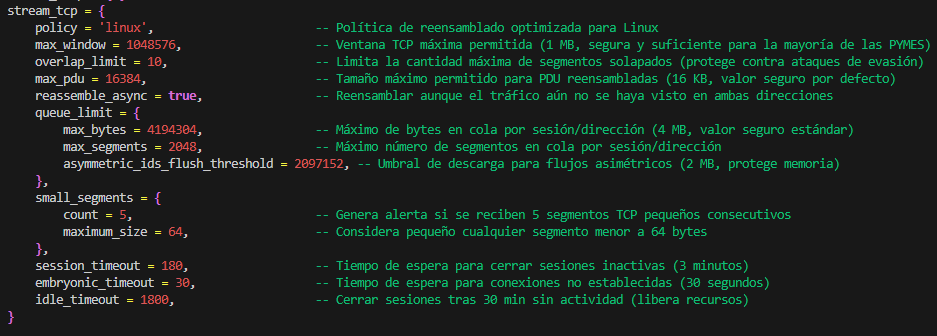
\includegraphics[scale=0.6]{stream_tcp/1.png}
	\caption{Configuración de Stream TCP.}
\end{figure}

\subsection{Reputation}

Este preprocesador permite bloquear IPs clasificadas como maliciosas utilizando listas negras. Para su funcionamiento se ha creado una carpeta \texttt{/reputation}, donde se almacena un archivo con IPs sospechosas, obtenidas del repositorio de \textit{emergingthreats.net} \cite{emerging_block_ips}. Esta funcionalidad es útil para evitar conexiones no deseadas hacia o desde nodos peligrosos.\newline

Como en los casos anteriores, tras configurar el módulo, se valida la sintaxis y se reinicia Snort para aplicar los cambios.

\begin{figure}[H]
	\centering
	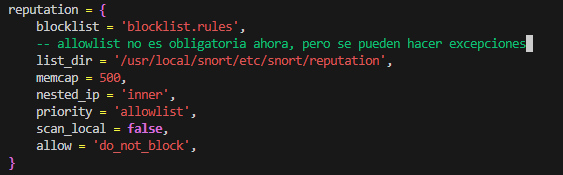
\includegraphics[scale=0.8]{reputation/1.png}
	\caption{Configuración de Reputation.}
\end{figure}

\newpage

\subsection{Datos sensibles}

En versiones anteriores de Snort existía el preprocesador \textit{Sensitive Data}, pero ha sido descontinuado en las versiones más recientes. Sin embargo, es posible emular parte de su funcionalidad adaptando expresiones regulares personalizadas que alerten sobre la presencia de datos sensibles típicos en el entorno de una PYME, como credenciales o números de tarjetas.\newline

Para ello, se crea un nuevo archivo de reglas llamado \texttt{custom.rules}, donde se definen patrones específicos a detectar.

\begin{figure}[H]
	\centering
	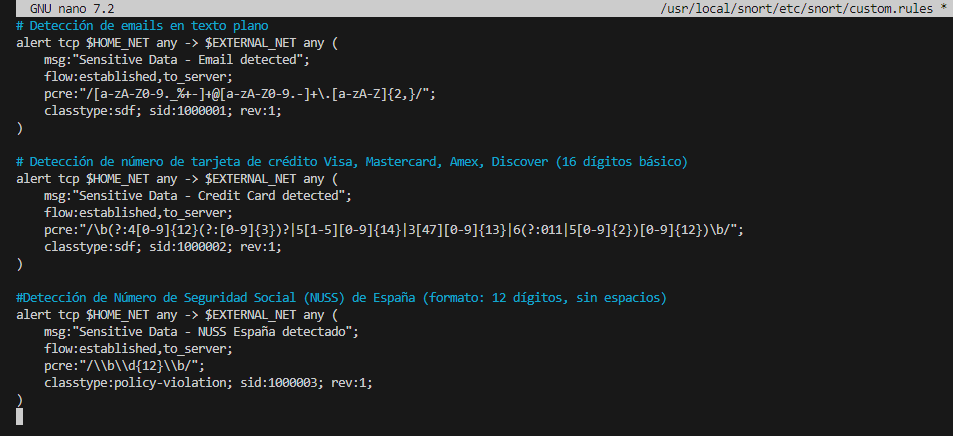
\includegraphics[scale=0.6]{sensitive/1.png}
	\caption{Expresiones regulares para protección de datos sensibles.}
\end{figure}

Posteriormente, se añade la ruta de este archivo en \texttt{snort.lua}, se comprueba la validez de la configuración utilizando \texttt{libdaq} y se reinicia el servicio para aplicar los cambios.

\begin{figure}[H]
	\centering
	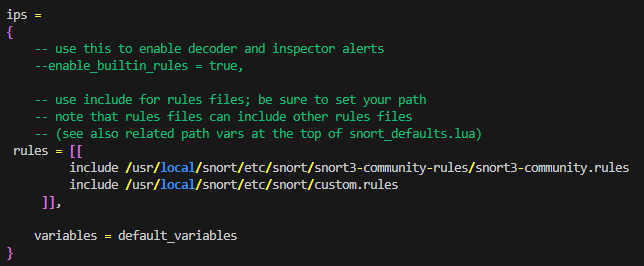
\includegraphics[scale=0.6]{sensitive/2.png}
	\caption{Agregación de \texttt{custom.rules}.}
\end{figure}

\pagebreak

\subsection{Antivirus ClamAV}

Finalmente, se procede con la instalación del antivirus \textbf{ClamAV}, una solución de código abierto utilizada para la detección de malware. Su integración complementa las capacidades de Snort mediante el análisis basado en firmas.

\begin{figure}[H]
	\centering
	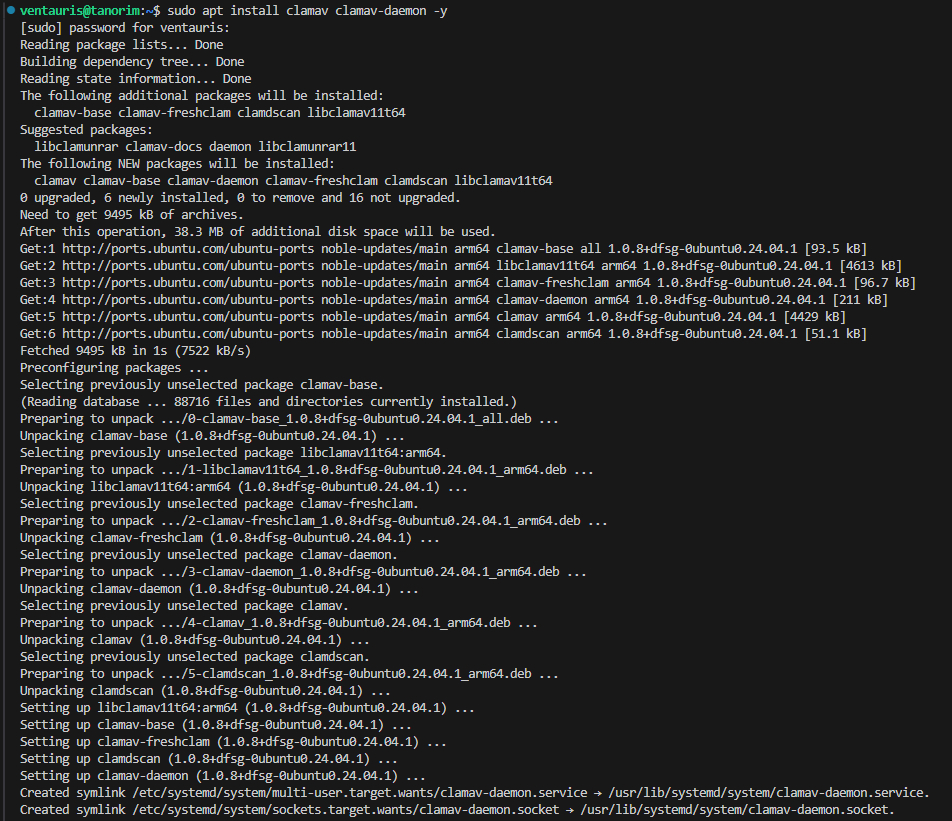
\includegraphics[scale=0.6]{clamAV/1.png}
	\caption{Instalación de ClamAV.}
\end{figure}

Tras la instalación, se detiene el servicio, se actualizan las firmas de virus y se reinicia el demonio para activar la protección.

\begin{figure}[H]
	\centering
	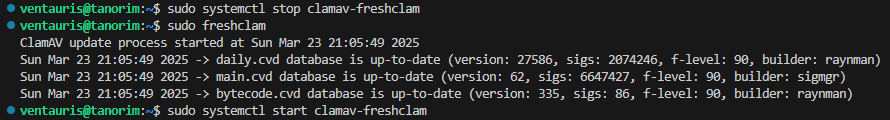
\includegraphics[scale=0.6]{clamAV/2.png}
	\caption{Actualización de firmas y reinicio del servicio ClamAV.}
\end{figure}


\newpage

%%%%%%%%%%%%%%%%%%HECHO5

\section{Generación de un script para la instalación automática}

\subsection{Esquema de red de monitorización con R-SNORT}

Para permitir la inspección total del tráfico en una red local, se diseñó un esquema de red específico que garantiza que todo el tráfico —tanto el generado entre dispositivos locales como el que entra y sale hacia Internet— pueda ser observado por el sistema \textbf{R-SNORT} de manera eficiente y no intrusiva.

\begin{figure}[H]
	\centering
	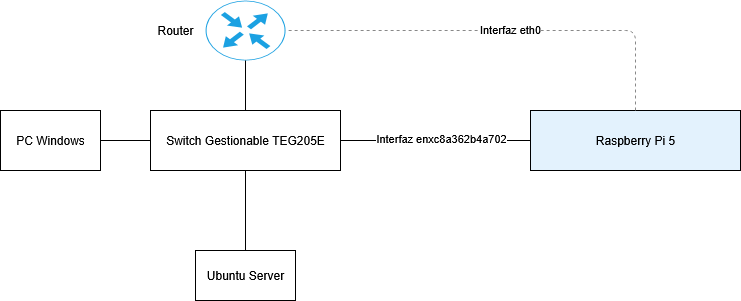
\includegraphics[scale=0.6]{script_automatico/network.png}
	\caption{Esquema de red real del proyecto.}
\end{figure}

\subsubsection{Descripción del esquema}

La red está compuesta por:

\begin{itemize}
	\item Un \textbf{switch gestionable} (modelo \texttt{Tenda TEG205E}) con capacidad de \textit{Port Mirroring}.
	\item Dos dispositivos cliente conectados a los puertos 2 y 3 del switch: un ordenador con \textbf{Windows} y una máquina con \textbf{Ubuntu Server}.
	\item Un \textbf{router doméstico} conectado al puerto 1 del switch, encargado de proporcionar acceso a Internet.
	\item Una \textbf{Raspberry Pi 5} equipada con dos interfaces de red Ethernet:
	\begin{itemize}
		\item \texttt{eth0}: conectada directamente al router, proporciona conectividad a Internet para la propia Raspberry Pi.
		\item \texttt{enxc8a362b4a702}: conectada al puerto 4 del switch, el cual está configurado como puerto espejo.
	\end{itemize}
\end{itemize}

El \textit{Port Mirroring} se configura para duplicar el tráfico de los puertos 1, 2 y 3 (los dispositivos productivos y el router) hacia el puerto 4, permitiendo que la interfaz \texttt{enxc8a362b4a702} de la Raspberry Pi capture de forma pasiva y en tiempo real todo el tráfico interno y externo de la red.

\subsubsection{Objetivo de este diseño}

El objetivo principal de esta arquitectura es que \textbf{R-SNORT} funcione como un sistema de detección de intrusiones pasivo (\textit{Network-based IDS}) sin interferir en el flujo de los datos. Para ello, deben cumplirse dos condiciones técnicas fundamentales:

\begin{enumerate}
	\item La interfaz utilizada para la captura debe operar en \textbf{modo promiscuo}, sin dirección IP asignada, actuando como una sonda pasiva totalmente invisible para el resto de la red.
	\item El switch debe soportar \textbf{duplicación de tráfico} (\textit{mirroring}) para garantizar que todo el tráfico relevante sea reenviado correctamente al puerto de análisis.
\end{enumerate}

\subsubsection{Justificación técnica}

Este tipo de arquitectura es común en entornos profesionales donde se desea realizar \textit{inspección profunda de paquetes} (\textit{Deep Packet Inspection}) sin introducir latencia ni crear puntos únicos de fallo en la red. Además, permite mantener completamente aislado el sistema IDS del resto de dispositivos, lo cual incrementa la seguridad del propio entorno de monitorización.\newline

La elección de una \textbf{Raspberry Pi 5} se justifica por su bajo consumo energético, su arquitectura ARM eficiente, y su capacidad para operar con interfaces Ethernet Gigabit, siempre que se utilice un adaptador USB 3.0 para incorporar una segunda interfaz de red.

\subsubsection{Alternativas descartadas}

Se valoró la posibilidad de implementar una arquitectura enrutada —donde todo el tráfico pasara a través de la Raspberry Pi—, sin embargo, esta solución presentaba varios inconvenientes:

\begin{itemize}
	\item Aumentaría la latencia y la carga de red para todos los dispositivos conectados.
	\item Requiere una configuración compleja de \texttt{NAT} o \texttt{bridging} en la Raspberry Pi.
	\item Introduce un punto único de fallo que compromete la disponibilidad de la red en caso de errores.
\end{itemize}

Por tanto, la arquitectura basada en un \textbf{switch con mirroring} y una sonda pasiva resulta significativamente más robusta, profesional y realista para el entorno de una pequeña o mediana empresa (\textbf{PYME}).


\subsection{Primera fase del script automático}
% Contenido de la sección 2.5
La instalación manual de \textit{Snort 3}, especialmente en dispositivos embebidos como la Raspberry Pi, puede convertirse en un proceso complejo y propenso a errores debido a la cantidad de dependencias, compilaciones desde código fuente y configuraciones específicas del sistema. Por este motivo, se ha desarrollado un script de instalación automática denominado \textbf{R-SNORT INSTALLER}, que encapsula todo el proceso de despliegue de manera modular, robusta y reproducible.

\subsubsection{Motivación y diseño modular}

Automatizar la instalación de herramientas en ciberseguridad como Snort es un paso habitual para garantizar la repetibilidad de los entornos de prueba, minimizar el error humano y facilitar la portabilidad entre dispositivos. Esta filosofía está alineada con los principios de \textit{Infrastructure as Code} (IaC), promovida en múltiples estudios recientes sobre automatización segura.
\newline

El script propuesto sigue una arquitectura modular, dividiendo su lógica en funciones independientes organizadas en ficheros temáticos:

\begin{itemize}
	\item \texttt{r-snort\_installer.sh}: núcleo del sistema, orquesta las fases del proceso de instalación desde una perspectiva modular, gestionando logs, permisos, selección de interfaz y llamadas a los demás módulos.  
	Véase la Figura~\ref{fig:r-snort_installer} para una muestra del flujo de ejecución principal.
	
	\item \texttt{core.sh}: módulo responsable de los mensajes de log, errores y el banner de bienvenida, garantizando una salida legible y profesional para el usuario.  
	Véase la Figura~\ref{fig:core-sh}.
	
	\item \texttt{checks.sh}: este módulo verifica que el script se ejecute como root y solicita al usuario que seleccione la interfaz de red sobre la que actuará Snort.  
	Representación visual en la Figura~\ref{fig:checks-sh}.
	
	\item \texttt{dependencies.sh}: instala los paquetes de compilación y bibliotecas necesarios en entornos Debian/Ubuntu.  
	La Figura~\ref{fig:dependencies-sh} muestra un fragmento de esta lógica.
	
	\item \texttt{build\_from\_source.sh}: gestiona y compila desde fuentes los componentes adicionales (luajit, daq, openssl, etc.).  
	También maneja errores comunes de compatibilidad, como se muestra a continuación:
	
	\begin{lstlisting}[language=bash, caption={Corrección de versiones incompatibles de xz/liblzma}, label=lst:xz, basicstyle=\ttfamily\footnotesize, frame=single, numbers=left, numberstyle=\tiny, breaklines=true]
		if ! xz -t "$archivo" 2>&1 | grep -qv 'version `XZ_'; then
		apt-get install --reinstall -y xz-utils liblzma5 liblzma-dev
		fi
	\end{lstlisting}
	
	\item \texttt{install\_snort.sh}: compila Snort 3.1.84.0 con correcciones específicas para evitar fallos con versiones recientes de OpenSSL y desactiva el soporte NUMA.  
	Véase la Figura~\ref{fig:install-snort}.
	
	\item \texttt{configure\_snort.sh}: prepara la configuración final de Snort, cargando reglas, scripts \texttt{.lua}, y desplegando el servicio con \texttt{systemd}.  
	Representado en la Figura~\ref{fig:configure-snort}.
	
	\item \texttt{swap.sh}: activa dinámicamente un archivo de swap temporal si se detecta menos de 1.5\,GB de RAM, evitando fallos de compilación en la Raspberry Pi.  
	Ver la Figura~\ref{fig:swap-sh}.
	
	\item \texttt{stats.sh}: recopila y presenta estadísticas del sistema tras la instalación, incluyendo versiones de Snort y ClamAV, recursos utilizados y configuración de red.  
	Ilustrado en la Figura~\ref{fig:stats-sh}.
\end{itemize}

\subsubsection{Características de robustez y control de errores}

El script implementa buenas prácticas de scripting en Bash, incluyendo:

\begin{itemize}
	\item Uso de \texttt{set -euo pipefail} para evitar ejecuciones silenciosas tras errores.
	\item Captura de errores con \texttt{trap} para identificar fallos que desestabilicen o anulen la instalación.
	\item Registro detallado en \texttt{/var/log/snort\_install.log} mediante redirección directa del flujo de salida.
\end{itemize}

Además, cada función de especial importancia o con condiciones de carrera se acompaña de validaciones explícitas. Por ejemplo, antes de descomprimir archivos \texttt{.tar.gz} o \texttt{.tar.xz}, se comprueba su integridad con \texttt{gzip -t} o \texttt{xz -t}, y se mitigan fallos comunes de \texttt{liblzma} con reinstalación forzada si es necesario.

\begin{lstlisting}[language=bash, caption={Validación e instalación segura de paquetes .xz}, label=lst:xz]
	if ! xz -t "$archivo" 2>&1 | grep -qv 'version `XZ_'; then
	apt-get install --reinstall -y xz-utils liblzma5 liblzma-dev
	fi
\end{lstlisting}

\subsubsection{Automatización total del servicio Snort}

Una vez instalado, \texttt{Snort} es configurado automáticamente como un servicio \texttt{systemd}. El script genera dinámicamente el archivo \texttt{snort.service} y lo enlaza al directorio correcto, con los parámetros adecuados de reinicio automático, límites de recursos y uso de la interfaz de red seleccionada interactivamente por el usuario.

\begin{lstlisting}[language=bash, caption={Sección relevante del systemd generado}, label=lst:systemd]
	[Service]
	ExecStart=/usr/local/snort/bin/snort -c /usr/local/snort/etc/snort/snort.lua -i eth0 -A alert_fast
	Restart=always
	User=root
	Group=root
\end{lstlisting}

\subsubsection{Mitigación de limitaciones de hardware}

Para abordar las limitaciones de memoria RAM propias de sistemas como la ARM (no presente en Raspberry Pi 5 de 8GB de RAM), el script evalúa si el sistema posee menos de 1.5GB de RAM y en ese caso crea un archivo de swap temporal de 2GB:

\begin{lstlisting}[language=bash]
	if [ "$mem_kb" -lt 1500000 ]; then
	fallocate -l 2G /swapfile_snort
\end{lstlisting}

Esta característica permite compilar Snort de forma estable incluso en configuraciones reducidas, evitando fallos durante la fase de \texttt{make -j\$(nproc)}.

\subsubsection{Instalación adicional de ClamAV y control antivirus}

Dado que el proyecto R-Snort está pensado como un sistema IDS autónomo para pequeñas y medianas empresas, se incluyó también la instalación automática de \texttt{ClamAV}, permitiendo disponer de un escáner antivirus activo desde el arranque. La instalación es completamente silenciosa y actualiza su base de firmas mediante \texttt{freshclam}.

\subsubsection{Resultados e impacto del diseño}

El instalador automático consigue reducir a menos de 15 minutos la instalación completa de Snort, desde dependencias hasta configuración funcional. Esta reducción de complejidad aumenta la fiabilidad y la reproducibilidad del entorno, dos factores muy demandados para sistemas de detección de intrusos.\newline

Además, se ha verificado que, tras una ejecución limpia del instalador, Snort queda operativo como servicio persistente, escuchando tráfico en tiempo real y generando alertas sobre tráfico malicioso, todo ello sin intervención posterior del usuario.

\pagebreak

%%%%%%%%%%%%HECHO6

\subsection{Transición a paquete \texttt{.deb}}

Con el objetivo de profesionalizar el despliegue de \textbf{R-SNORT} y facilitar su uso en entornos reales, se reestructuró el proyecto como un paquete Debian estándar. Esta decisión permite que el propio sistema operativo gestione la instalación, dependencias, configuración y servicio a través de scripts como \texttt{postinst} (ver Figura~\ref{fig:postinst}), \texttt{prerm} (ver Figura~\ref{fig:prerm}) y \texttt{postrm} (ver Figura~\ref{fig:postrm}), alineándose con las buenas prácticas del ecosistema Debian.
\newline

El resultado es una arquitectura empaquetada bajo el nombre \texttt{r-snort-deb.deb}, que se instala fácilmente mediante un único comando y permite revertir el proceso de instalación sin dejar rastros en el sistema.

\begin{figure}[H]
	\centering
	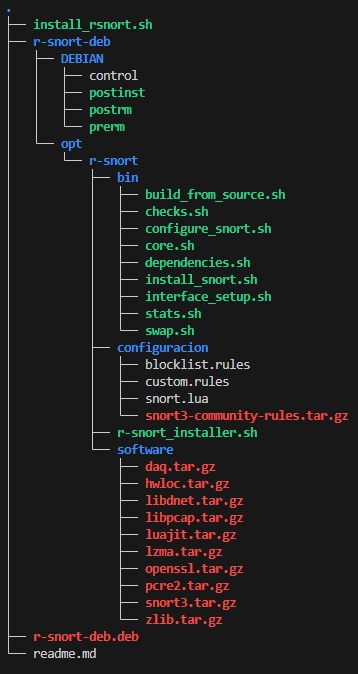
\includegraphics[scale=0.8]{script_automatico/13.png}
	\caption{Estructura del proyecto reempaquetado como archivo \texttt{.deb}.}
\end{figure}

\subsubsection{Mejoras introducidas}

La transición al formato \texttt{.deb} permitió incorporar una serie de mejoras que anteriormente solo podían aplicarse de forma manual:

\begin{itemize}
	\item \textbf{Selección dinámica de interfaz:} se desarrolló un script de instalación previa, \texttt{install\_rsnort.sh} (ver Figura~\ref{fig:install_rsnort}), que detecta automáticamente las interfaces Ethernet disponibles y permite al usuario seleccionar la que se conectará al puerto espejo del switch. La elección se guarda en \texttt{/etc/rsnort\_iface} para que pueda ser utilizada posteriormente por otros componentes del sistema.
	
	\item \textbf{Modo promiscuo y sin IP:} se creó el script \texttt{interface\_setup.sh} (ver Figura~\ref{fig:interface_setup}) que activa automáticamente la interfaz seleccionada, elimina cualquier dirección IP existente para evitar conflictos, y la configura en modo \textit{promiscuo}. Este paso es esencial para que Snort pueda inspeccionar todo el tráfico redirigido desde el switch sin interferir en el funcionamiento de la red.
	
	\begin{lstlisting}[language=bash, caption={Activación automática del modo promiscuo en interface\_setup.sh}, label=lst:promiscuo, basicstyle=\ttfamily\footnotesize, frame=single, numbers=left, numberstyle=\tiny, breaklines=true]
	if [[ "$state" != "UP" ]]; then
		ip link set dev "$iface" up
	fi
	
	ip addr flush dev "$iface"
	ip link set "$iface" promisc on
	\end{lstlisting}
	
	\item \textbf{Despliegue como servicio \texttt{systemd}:} se redefinió el proceso de inicio de Snort mediante una unidad personalizada de \texttt{systemd}, lo que permite un arranque automático, supervisión y control del servicio tras cada reinicio del sistema.
	
	\item \textbf{Fortalecimiento con ClamAV:} para añadir una capa extra de protección, se integró la instalación y activación automática del antivirus ClamAV. Esto es especialmente útil en entornos donde Snort pueda capturar tráfico de archivos potencialmente contaminados o vectores de malware.
\end{itemize}

\subsubsection{Justificación del rediseño}

Este rediseño responde no solo a criterios técnicos, sino también a aspectos de usabilidad. En entornos reales, como pequeñas y medianas empresas (PYMEs), que desean adoptar soluciones \textit{NIDS}, es esencial que la herramienta pueda instalarse, configurarse y mantenerse sin requerir conocimientos avanzados en administración de sistemas. Gracias a esta transición, \textbf{R-SNORT} puede considerarse una solución \textit{plug-and-play}:

\begin{enumerate}
	\item El usuario ejecuta \texttt{install\_rsnort.sh} (ver Figura~\ref{fig:install_rsnort}).
	\item Selecciona la interfaz conectada al switch mediante un menú interactivo.
	\item El paquete se instala y configura automáticamente, sin intervención adicional.
\end{enumerate}

Esta arquitectura modular empaquetada sigue las mejores prácticas de la ingeniería de software y permite escalar, actualizar o personalizar R-SNORT en futuras versiones con mínima fricción.

\pagebreak

\subsubsection{Resultado final}

Gracias a la evolución hacia un paquete \texttt{.deb}, \textbf{R-SNORT} se consolida como una herramienta más robusta, mantenible y amigable con el usuario final. Es importante recordar que este proyecto busca ofrecer una solución eficaz, ligera y accesible para redes SOHO (\textit{Small Office / Home Office}). Con un enfoque modular interno y una experiencia de instalación unificada, el sistema mantiene toda su capacidad de inspección avanzada sin renunciar a la simplicidad en su despliegue.

%HECHO7


\chapter{Casos prácticos: utilización de R-Snort}

\section{Entorno de trabajo}

El sistema R-Snort ha sido desplegado en un entorno de red realista a pequeña escala, compuesto por los siguientes elementos:

\begin{itemize}
	\item Una Raspberry Pi 5 con sistema operativo Ubuntu Server, encargada de ejecutar el paquete automatizado con Snort.
	\item Un switch gestionable Tenda TEG205E, configurado para replicar todo el tráfico de red mediante la funcionalidad de \textit{port mirroring}.
	\item Un adaptador UGREEN USB 3.0 a Ethernet Gigabit conectado a la Raspberry, que actúa como interfaz de captura para Snort.
	\item Un router doméstico (F@st 5670) que proporciona conectividad a Internet a toda la red.
	\item Dos equipos cliente: un PC con Windows y otro con Ubuntu Server, ambos conectados al switch.
\end{itemize}

El puerto 4 del switch se ha configurado como destino del \textit{mirroring}, recibiendo una copia del tráfico de los puertos 1 a 3 (correspondientes al router y los dos PCs). De esta manera, R-Snort es capaz de recibir una copia tanto del tráfico interno como del proveniente de Internet. La Raspberry escucha dicho tráfico a través del adaptador UGREEN, el cual se configura automáticamente en modo promiscuo, sin dirección IP asignada, para evitar interferencias en la red.

\section{Instalación}

La instalación se ha simplificado al máximo para que cualquier usuario pueda desplegar R-Snort sin conocimientos técnicos avanzados. El proceso consta de dos fases principales:

\begin{enumerate}
	\item Ejecución del script \texttt{install\_rsnort.sh}, que actualiza paquetes, instala dependencias y solicita al usuario que seleccione la interfaz de red conectada al switch.
	\item Instalación del paquete \texttt{.deb}, que compila Snort y sus dependencias, configura la interfaz en modo promiscuo, crea el servicio en \texttt{systemd}, e inicia automáticamente el demonio de Snort.
\end{enumerate}

A continuación, se presentan algunas capturas del proceso, incluyendo tanto la preparación del hardware como de la instalación software:\newline

La Raspberry Pi 5 cuenta con dos interfaces Ethernet: una conectada directamente al router para acceder a Internet desde fuera de la red local (\texttt{eth0}), y otra a través de un adaptador USB 3.0 (UGREEN) destinada exclusivamente a capturar tráfico de red (\texttt{enxc8a362b4a702}). Esta segunda interfaz es la que recibe todo el tráfico replicado desde el switch mediante \textit{port mirroring}.

\begin{figure}[H]
	\centering
	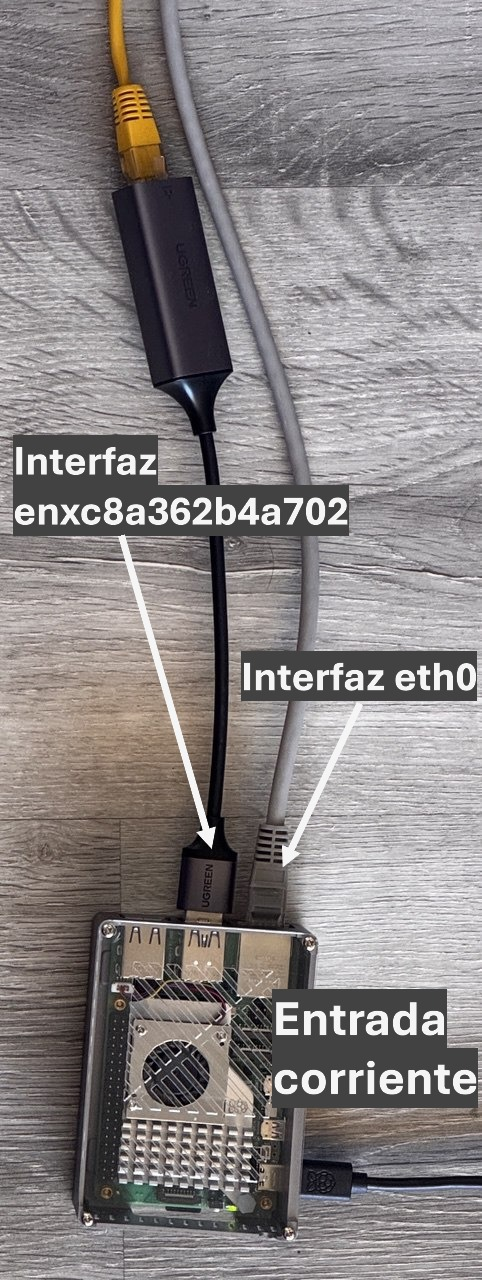
\includegraphics[width=0.35\textwidth]{pruebas_config/1-1.JPG}
	\caption{Raspberry Pi conectada con dos interfaces Ethernet.}
\end{figure}

\pagebreak

\subsection*{Asignación de dispositivos al switch}

El switch gestionable Tenda permite configurar el tráfico de cada puerto. En este caso, se conectaron el router, los dos PCs (Windows y Ubuntu Server) y la Raspberry Pi. Esta última se conecta a un puerto configurado como espejo de los demás, lo que le permite capturar el tráfico replicado.

\begin{figure}[H]
	\centering
	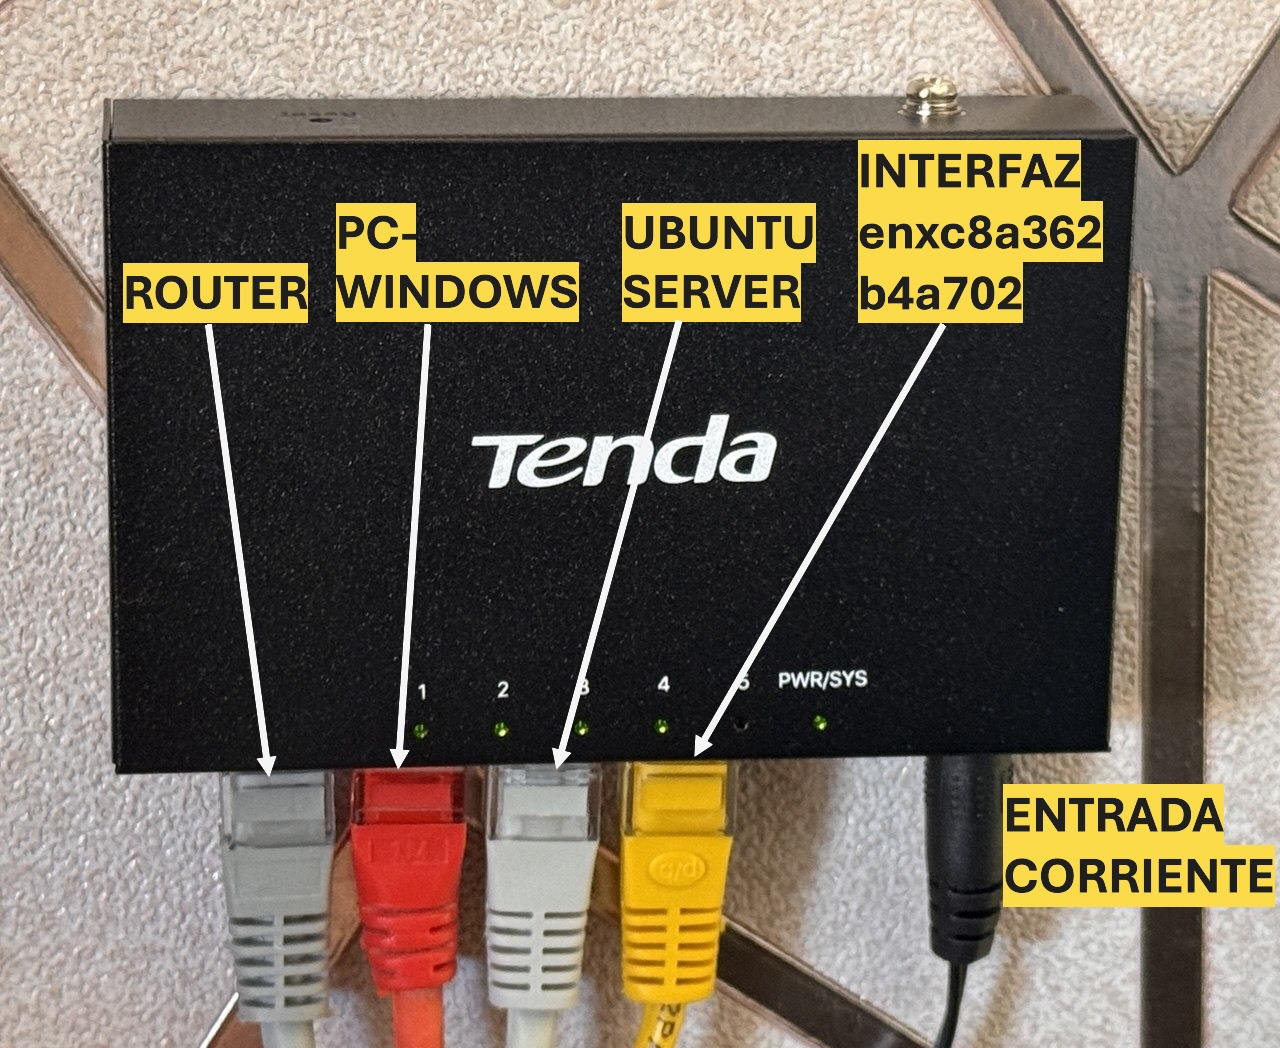
\includegraphics[width=0.65\textwidth]{pruebas_config/2-2.JPG}
	\caption{Conexiones físicas al switch gestionable.}
\end{figure}

\subsection*{Identificación del entorno LAN}

Desde la interfaz web del router se pueden visualizar todos los dispositivos conectados. Esto permite verificar que tanto el switch como la Raspberry Pi están correctamente integrados en la red y responden a su dirección IP.

\begin{figure}[H]
	\centering
	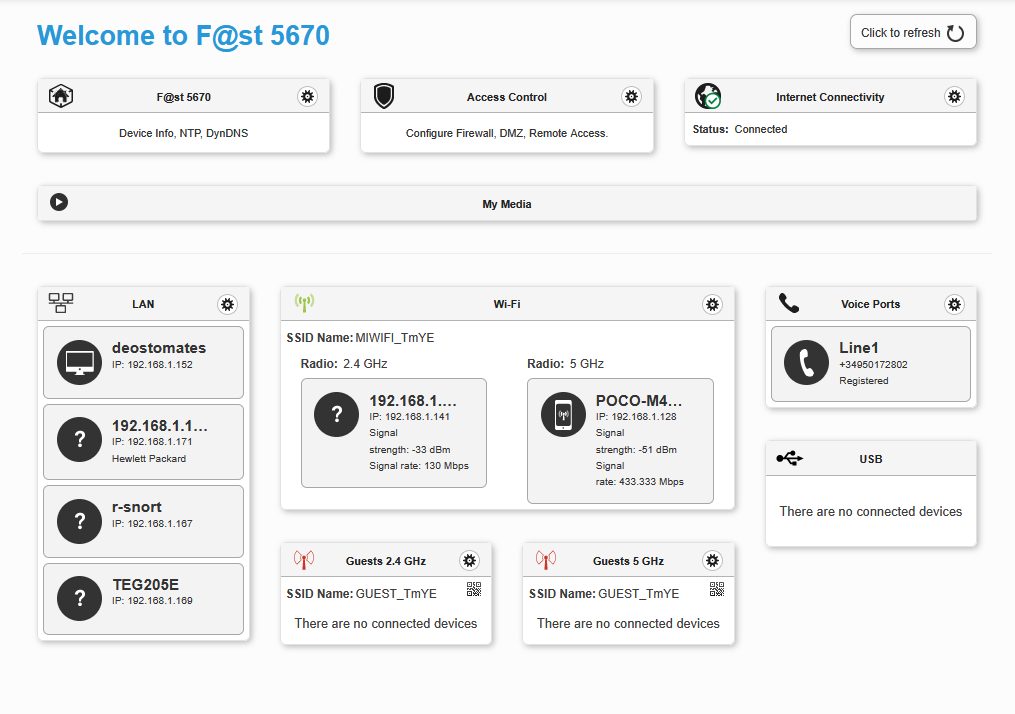
\includegraphics[width=0.65\textwidth]{pruebas_config/3-router.png}
	\caption{Dispositivos visibles en la red doméstica.}
\end{figure}

\subsection*{Acceso al switch Tenda}

Para configurar el port mirroring es necesario acceder al panel web del switch. Para ello, se localiza su dirección IP desde el router (192.168.1.169) y se accede a ella mediante un navegador web.

\begin{figure}[H]
	\centering
	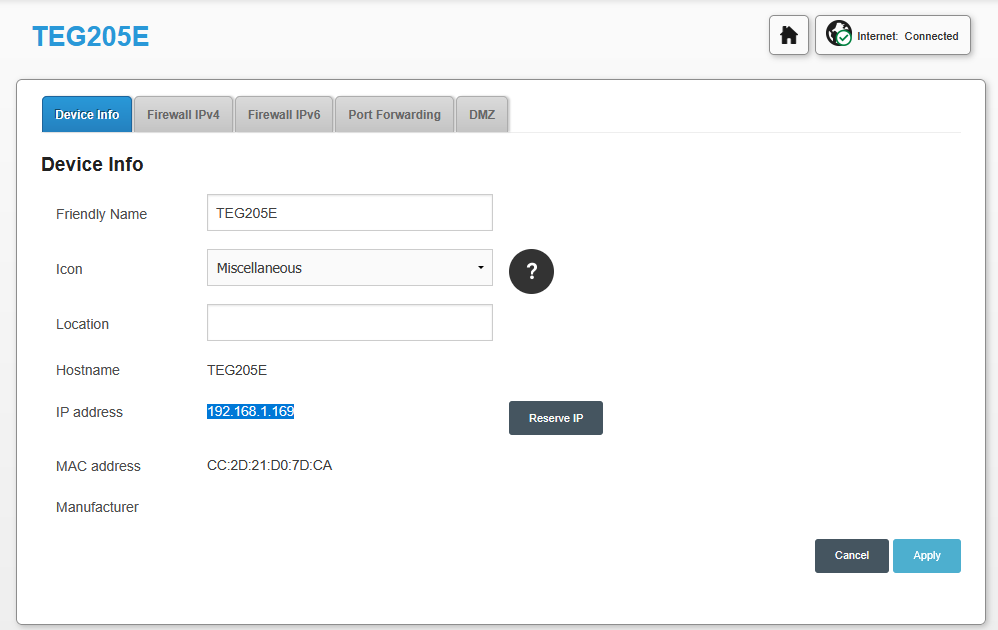
\includegraphics[width=0.65\textwidth]{pruebas_config/4-localizar_tenda.png}
	\caption{IP local del switch detectada desde el router.}
\end{figure}

\begin{figure}[H]
	\centering
	
\includegraphics[width=0.5\textwidth]{pruebas_config/5-tenda_web.png}
	\caption{Pantalla de acceso al panel de administración.}
\end{figure}

\pagebreak

\subsection*{Seguridad inicial del dispositivo}

En el primer acceso al switch, el sistema solicita el cambio obligatorio de la contraseña predeterminada para mejorar la seguridad del entorno.

\begin{figure}[H]
	\centering
	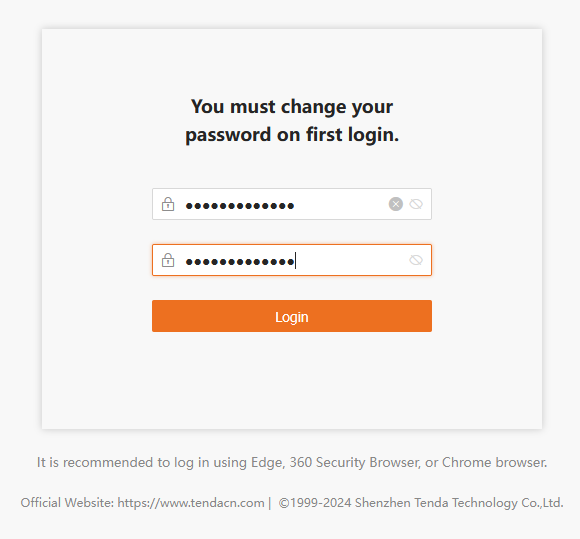
\includegraphics[width=0.5\textwidth]{pruebas_config/6-cambio_pass_tenda.png}
	\caption{Cambio obligatorio de contraseña en el primer inicio.}
\end{figure}

\subsection*{Configuración avanzada del switch}

Una vez autenticados, accedemos a la interfaz de administración, donde es posible configurar diversos parámetros del dispositivo. Desde esta sección se define el \textit{port mirroring}, se habilitan o deshabilitan puertos y se monitoriza el estado de la red.

\begin{figure}[H]
	\centering
	\includegraphics[width=0.8\textwidth]{pruebas_config/7-pagina_tenda.png}
	\caption{Vista general del panel de gestión del switch.}
\end{figure}

\pagebreak

\subsection*{Activación del Port Mirroring}

Desde el apartado \texttt{switching > port mirroring}, activamos esta funcionalidad para duplicar el tráfico de red. Se configura el switch para replicar el tráfico de los puertos donde están conectados el router y los PCs (puertos 1, 2 y 3) hacia el puerto 4, que está vinculado a la interfaz de análisis de la Raspberry Pi. Esto permite que Snort reciba una copia completa del tráfico local y externo.

\begin{figure}[H]
	\centering
	\includegraphics[width=0.65\textwidth]{pruebas_config/9-asignacion_port.png}
	\caption{Verificación del estado de los puertos tras la configuración.}
\end{figure}

\pagebreak

Finalmente, ejecutamos como administrador el script \texttt{installer\_snort.sh} para iniciar la instalación de R-Snort. Se selecciona la interfaz de red correspondiente al puerto 4 del switch, que es el que recibe el tráfico duplicado. Una vez finalizado el proceso, el sistema queda completamente operativo. El código fuente del instalador puede consultarse en el Anexo~\ref{anexo_repositorio}.

\begin{figure}[H]
	\centering
	\begin{minipage}[b]{0.48\textwidth}
		\centering
		\includegraphics[scale=0.4]{script_automatico/14.png}
		\caption*{(a) Ejecución de R-Snort.}
	\end{minipage}
	\hfill
	\begin{minipage}[b]{0.48\textwidth}
		\centering
		\includegraphics[scale=0.4]{pruebas_config/10-10.png}
		\caption*{(b) Finalización del instalador.}
	\end{minipage}
	\caption{Proceso completo de instalación automática de R-Snort.}
\end{figure}

%HECHO8

% --> Aquí se insertan las figuras

\section{Utilización y pruebas}

Una vez completada la instalación, se procedió a la validación funcional del sistema y a su evaluación de rendimiento. El objetivo principal es demostrar que R-Snort es capaz de monitorizar eficazmente todo el tráfico de red y detectar amenazas sin saturar los recursos del sistema.

\subsection{Benchmark de rendimiento}

\subsubsection{Metodología}

Para medir el rendimiento de R-Snort, se utilizó la herramienta \texttt{dstat}, que permite monitorizar en tiempo real diversos parámetros del sistema, como el uso de CPU, memoria, red y disco. Se realizaron dos sesiones de captura de datos:

\begin{itemize}
	\item Una con Snort encendido y funcionando en modo \textit{inline}, procesando el tráfico en tiempo real.
	\item Otra con Snort completamente apagado, lo que permitió establecer una línea base del consumo del sistema sin el IDS.
\end{itemize}

Cada sesión de monitoreo generó un archivo CSV con un intervalo de muestreo de 1 segundo, que posteriormente fue procesado para generar gráficas comparativas. Se utilizó Python, junto con las bibliotecas \texttt{pandas} y \texttt{matplotlib}, para el análisis y visualización de datos.

\subsubsection{Resultados e interpretación de gráficas}

A continuación, se presentan las gráficas obtenidas:

\begin{figure}[H]
	\centering
	\includegraphics[width=\textwidth]{graficas/net_recv.png}
	\caption{Red: Bytes recibidos por segundo}
\end{figure}
\textbf{Análisis:} Se observa un patrón de tráfico más irregular y, en ocasiones, más intenso cuando Snort está apagado. Con Snort activo, el tráfico parece más contenido, probablemente porque parte de los paquetes son descartados o procesados de forma más lenta. Esto sugiere una influencia directa del IDS sobre el tráfico recibido.

\begin{figure}[H]
	\centering
	\includegraphics[width=\textwidth]{graficas/net_send.png}
	\caption{Red: Bytes enviados por segundo}
\end{figure}
\textbf{Análisis:} El patrón de tráfico enviado es bajo en ambas sesiones, aunque con Snort encendido se detecta un ligero aumento en los picos. Esto puede deberse a respuestas generadas por Snort tras detectar actividad anómala, como en pruebas de copia de datos o escaneo de puertos.

\begin{figure}[H]
	\centering
	\includegraphics[width=\textwidth]{graficas/context_switch.png}
	\caption{Context switches por segundo}
\end{figure}
\textbf{Análisis:} El número de cambios de contexto se incrementa notablemente con Snort activo. Este comportamiento es esperable, ya que el análisis en tiempo real de paquetes obliga al sistema a alternar con mayor frecuencia entre procesos.

\begin{figure}[H]
	\centering
	\includegraphics[width=\textwidth]{graficas/cpu_idle.png}
	\caption{CPU inactiva (\%)}
\end{figure}
\textbf{Análisis:} La CPU permanece prácticamente inactiva cuando Snort está apagado. Al activarlo, se reduce levemente el porcentaje de inactividad, indicando un impacto ligero pero constante sobre el procesador.

\begin{figure}[H]
	\centering
	\includegraphics[width=\textwidth]{graficas/cpu_sys.png}
	\caption{Uso de CPU del sistema (\%)}
\end{figure}
\textbf{Análisis:} Se observa un aumento en el uso de CPU en espacio de sistema con Snort activo. Este comportamiento es coherente con el hecho de que el IDS opera en niveles bajos, haciendo uso intensivo de bibliotecas como \texttt{libpcap} para la captura de paquetes.

\begin{figure}[H]
	\centering
	\includegraphics[width=\textwidth]{graficas/cpu_usr.png}
	\caption{Uso de CPU del usuario (\%)}
\end{figure}
\textbf{Análisis:} El impacto en el espacio de usuario es moderado. Aunque no se alcanzan valores elevados, la diferencia entre tener Snort encendido o apagado es clara, reflejando la carga asociada al motor de detección.

\begin{figure}[H]
	\centering
	\includegraphics[width=\textwidth]{graficas/disk_read.png}
	\caption{Lectura de disco (B/s)}
\end{figure}
\textbf{Análisis:} No se detectan lecturas de disco relevantes en ninguna de las dos sesiones. Este resultado es esperado, dado que Snort opera principalmente en memoria RAM y no realiza accesos intensivos a disco en su modo de funcionamiento habitual.

\begin{figure}[H]
	\centering
	\includegraphics[width=\textwidth]{graficas/disk_write.png}
	\caption{Escritura de disco (B/s)}
\end{figure}
\textbf{Análisis:} Se registra un aumento significativo en la escritura en disco cuando Snort está activo, correspondiente a la generación de logs y alertas de seguridad.

\begin{figure}[H]
	\centering
	\includegraphics[width=\textwidth]{graficas/mem_used.png}
	\caption{Memoria usada (bytes)}
\end{figure}
\textbf{Análisis:} El uso de memoria crece de forma progresiva cuando Snort está encendido. Esto se debe a la carga de reglas, buffers de captura y estructuras internas del IDS. Al desactivarlo, el consumo de RAM disminuye considerablemente.

\pagebreak

En conjunto, estos resultados permiten concluir que R-Snort es eficiente y tiene un impacto reducido sobre el sistema en términos de consumo de recursos. No obstante, su actividad es claramente detectable, lo cual es esperable para un sistema de detección de intrusos activo y en tiempo real.\newline

Las pruebas de rendimiento se han enfocado en dos métricas principales:

\begin{itemize}
	\item \textbf{Carga del sistema:} se monitorizó el uso de CPU y RAM bajo escenarios de carga de red baja, media y alta. Esto se realizó utilizando herramientas como \texttt{htop}, \texttt{free -h} y el script de estadísticas internas de R-Snort.
	\item \textbf{Capacidad de análisis:} se evaluó la cantidad de paquetes por segundo que Snort puede procesar sin pérdidas ni errores, mediante herramientas de generación de tráfico como \texttt{iperf3} y \texttt{ping flood} desde los dos PCs.
\end{itemize}

Para poner estos datos en contexto, se compararon con estudios previos presentes en la literatura sobre el rendimiento de sistemas IDS en dispositivos embebidos. Los resultados obtenidos confirman que R-Snort ofrece un rendimiento competitivo incluso en hardware de bajo consumo.


\subsection{Pruebas}

Se han llevado a cabo distintas pruebas funcionales para verificar el correcto comportamiento del sistema:

\begin{itemize}
	\item \textbf{Detección de escaneos:} se lanzó un escaneo Nmap desde el PC con Ubuntu Server al equipo con Windows, generándose correctamente alertas visibles en el panel web.
	\item \textbf{Generación de tráfico legítimo:} navegación web, transferencia de archivos y conexión SSH, asegurando que Snort discrimina adecuadamente entre tráfico benigno y potencialmente malicioso.
	\item \textbf{Visualización en el panel web:} las alertas generadas por Snort se muestran en tiempo real en el dashboard desarrollado con Angular y Spring Boot.
\end{itemize}

Estas pruebas confirman que el sistema funciona de forma autónoma, detecta tráfico relevante sin incurrir en falsos positivos masivos y expone la información de manera clara y accesible para el usuario final.\newline

A continuación, se presentan pruebas reales ejecutadas en el entorno definido anteriormente (ver sección de topología de red), en las que R-Snort demuestra su capacidad de detección a través de reglas personalizadas y comunitarias. Cada caso incluye la alerta generada y una breve explicación técnica.

\vspace{0.5cm}

\subsubsection*{1. PINGs malformados y tráfico ICMP inusual}

Desde el equipo Ubuntu Server (\texttt{192.168.1.171}) se ejecutó un ping continuo hacia Google DNS (\texttt{8.8.8.8}):

\begin{verbatim}
	ping 8.8.8.8
\end{verbatim}

Snort generó múltiples alertas relacionadas con tráfico ICMP, incluyendo paquetes tipo \texttt{Unix ping}, \texttt{Echo reply} y PINGs anómalos. Esto confirma el correcto funcionamiento de los preprocesadores \texttt{stream}, \texttt{icmp} y la inspección de TTLs habilitada en \texttt{stream\_ip}.

\textbf{Configuración personalizada validada:} ajuste de parámetros como \texttt{min\_ttl}, \texttt{max\_overlaps} y \texttt{policy} en el bloque \texttt{stream\_ip}.

\begin{figure}[H]
	\centering
	\includegraphics[width=\textwidth]{pruebas/3.png}
	\caption{Tráfico ICMP detectado por preprocesadores y reglas comunitarias.}
\end{figure}

\vspace{0.5cm}

\subsubsection*{2. Fugas de datos sensibles (emails y tarjetas)}

Se evaluó el funcionamiento de las reglas definidas en \texttt{custom.rules}, simulando la filtración de datos confidenciales desde Ubuntu hacia el router:

\begin{verbatim}
	curl -d "Mi email es prueba@ejemplo.com" http://192.168.1.1
	curl -d "Mi tarjeta es 4111111111111111" http://192.168.1.1
\end{verbatim}

Snort detectó ambas cadenas mediante expresiones regulares, generando alertas en tiempo real por detección de datos sensibles.

\textbf{Configuración personalizada validada:} uso de reglas propias con \texttt{pcre} y \texttt{flow}, integradas correctamente desde \texttt{custom.rules} en el archivo \texttt{snort.lua}.

\begin{figure}[H]
	\centering
	\includegraphics[width=\textwidth]{pruebas/4.png}
	\caption{Alertas generadas por reglas personalizadas ante filtraciones de datos.}
\end{figure}

\vspace{0.5cm}

\subsubsection*{3. Tráfico DNS sospechoso detectado automáticamente}

Sin necesidad de ejecutar comandos específicos, Snort detectó respuestas DNS con TTL muy bajo y sin autoridad, consideradas como posibles intentos de \textit{spoofing}.

Estas alertas se originaron durante la navegación web desde el PC con Windows, demostrando la efectividad de las reglas comunitarias aplicadas sobre el módulo DNS.

\textbf{Configuración personalizada validada:} activación del módulo \texttt{dns} mediante los bloques \texttt{binder} y \texttt{default\_mod} en \texttt{snort.lua}.

\begin{figure}[H]
	\centering
	\includegraphics[width=\textwidth]{pruebas/2.png}
	\caption{Respuestas DNS con TTL anómalo detectadas como tráfico malicioso.}
\end{figure}

\vspace{0.5cm}

\subsubsection*{4. Escaneo SNMP detectado con Nmap}

Se realizó un escaneo UDP desde el Ubuntu Server al equipo Windows para evaluar la detección de tráfico SNMP:

\begin{verbatim}
	sudo nmap -sU -p 161,705 192.168.1.152
\end{verbatim}

Snort identificó intentos de conexión tanto al puerto SNMP clásico como al puerto de AgentX, clasificándolos como intentos de reconocimiento o fuga de información.

\textbf{Configuración personalizada validada:} activación explícita de \texttt{rpc\_decode} y \texttt{snmp} en \texttt{snort.lua}, además de reglas comunitarias específicas para tráfico SNMP.

\begin{figure}[H]
	\centering
	\includegraphics[width=\textwidth]{pruebas/5.png}
	\caption{Detección de actividad SNMP sospechosa tras escaneo dirigido.}
\end{figure}

\vspace{0.5cm}

\subsubsection*{5. Detección de NUSS (Número de Seguridad Social)}

Se evaluó una regla personalizada para detectar cadenas numéricas de 12 dígitos que simulan un NUSS español. Desde el equipo Ubuntu se ejecutó:

\begin{verbatim}
	curl -d "Mi número de SSN es 123456789012" http://192.168.1.1
\end{verbatim}

Snort detectó la cadena como una posible violación de privacidad, generando una alerta con la clasificación y prioridad definidas manualmente.\newline

\textbf{Configuración personalizada validada:} expresión regular para patrones tipo NUSS, con una \texttt{classtype} propia y prioridad 1.

\begin{figure}[H]
	\centering
	\includegraphics[width=\textwidth]{pruebas/6.png}
	\caption{Alerta generada por la regla personalizada de detección de NUSS.}
\end{figure}

\section{Resumen}

Una vez completada la instalación de R-Snort, se ha evaluado su comportamiento en un entorno de red real, midiendo tanto su impacto en los recursos de la Raspberry Pi como su capacidad de detección. Para ello, se utilizó la herramienta \texttt{dstat} con el fin de comparar el rendimiento del sistema con Snort activado y desactivado. Los resultados indican que, aunque se observa un incremento en el uso de CPU, memoria y escritura en disco, dicho impacto es moderado y asumible para un dispositivo de recursos limitados. Asimismo, el tráfico de red presenta una leve alteración con Snort activo, lo que sugiere una ligera contención de paquetes provocada por el procesamiento en tiempo real.\newline

Además, se llevaron a cabo pruebas prácticas orientadas a validar las capacidades de detección del sistema. Acciones como escaneos de puertos con \texttt{Nmap} o el envío de datos sensibles (correos electrónicos, números de tarjeta o NUSS) fueron correctamente identificadas y notificadas mediante alertas. El sistema demostró una buena capacidad de diferenciación entre tráfico legítimo (por ejemplo, navegación web, transferencia de archivos o pings) y actividades potencialmente maliciosas. Estas alertas fueron reflejadas de forma inmediata en el panel web desarrollado, validando la integración completa entre el motor de detección y la interfaz de visualización.\newline

En conjunto, los resultados confirman que R-Snort es una solución eficaz para proteger redes pequeñas, ofreciendo capacidades avanzadas de detección sin comprometer el rendimiento del sistema ni la experiencia de usuario.


% Resultados y discusión
\chapter*{Resultados y discusión}
\addcontentsline{toc}{chapter}{Resultados y discusión}
% Contenido de resultados y discusión

% Conclusiones
\chapter*{Conclusiones}
\addcontentsline{toc}{chapter}{Conclusiones}

Tras las pruebas realizadas con R-Snort y el análisis del tráfico real, se concluye que el sistema presenta un consumo de recursos moderado y perfectamente asumible. Aunque se observa un incremento en la actividad de la CPU y la memoria cuando el motor de Snort está activo, el sistema permanece estable y responde adecuadamente en todo momento. Resulta destacable el rendimiento de la Raspberry Pi, que, a pesar de sus limitaciones de hardware, soporta con solvencia la carga asociada a la monitorización en tiempo real.\newline

Durante la fase de pruebas, R-Snort logró detectar una amplia variedad de eventos, desde peticiones ICMP simples (como \texttt{ping} hacia \texttt{8.8.8.8}) hasta escaneos de puertos mediante \texttt{Nmap}, pasando por intentos simulados de fuga de información con datos sensibles como correos electrónicos o números de tarjeta de crédito. En todos los casos, el sistema generó alertas precisas y en tiempo real.\newline

Un aspecto especialmente relevante es que la inspección continua del tráfico no interfiere de manera perceptible con el uso cotidiano de la red. Durante tareas como navegación web, descarga de archivos o conexiones SSH, el rendimiento se mantuvo fluido, lo que demuestra que R-Snort puede operar como una sonda pasiva sin afectar negativamente la experiencia del usuario. Incluso ante picos de tráfico, el sistema continúa funcionando de forma aceptable, aunque con una carga adicional esperada en el procesador.\newline

En resumen, desplegar R-Snort en un dispositivo tan compacto como una Raspberry Pi proporciona una solución de monitorización efectiva, de bajo impacto y con resultados fiables. Su capacidad para detectar comportamientos anómalos, generar alertas útiles y operar de forma transparente en la red lo convierten en una herramienta idónea para entornos domésticos o pequeñas oficinas, ofreciendo una capa adicional de seguridad sin requerir una infraestructura compleja ni costosa.


% Bibliografía
\begin{thebibliography}{29}
	
	\bibitem{enisa_smes}
	European Union Agency for Cybersecurity (ENISA). \textit{Cybersecurity for SMEs: Challenges and Recommendations}, 2021. Disponible en: \url{https://www.enisa.europa.eu/sites/default/files/publications/ENISA%20Report%20-%20Cybersecurity%20for%20SMES%20Challenges%20and%20Recommendations.pdf}. Último acceso: 9 abril 2025.
	
	\bibitem{rodriguez2018cluster}
	Rodríguez Eguren, P. S., Chichizola, F., y Rucci, E. (2018). \textit{Análisis del uso de un cluster de Raspberry Pi para cómputo de alto rendimiento}. En XXIV Congreso Argentino de Ciencias de la Computación (CACIC 2018), La Plata, Argentina, pp. 134-144. Disponible en: \url{http://sedici.unlp.edu.ar/handle/10915/73047}. Último acceso: 9 abril 2025.
	
	\bibitem{roesch1999snort}
	M. Roesch, ``Snort: Lightweight Intrusion Detection for Networks,'' en \textit{Proceedings of the 13th USENIX Conference on System Administration (LISA '99)}, Seattle, Washington, USA, 1999. Disponible en: \url{https://www.usenix.org/legacy/event/lisa99/full_papers/roesch/roesch.pdf}.
	
	\bibitem{snort3_official}
	Cisco Systems. \textit{Snort 3 Official Website}. Disponible en: \url{https://www.snort.org/snort3}. Último acceso: 9 abril 2025.
	
	\bibitem{insani2023implementation}
	Insani, P. P., Kanedi, I., y Al Akbar, A. (2023). \textit{Implementation of Snort as a Wireless Network Security Detection Tool Using Linux Ubuntu}. *Jurnal Komputer, Informasi dan Teknologi*, 3(2), 443--458.
	
	\bibitem{gkamas2022performance}
	Gkamas, T., Karaiskos, V., y Kontogiannis, S. (2022). \textit{Performance evaluation of distributed database strategies using Docker as a Service for industrial IoT data: Application to Industry 4.0}. *Information*, 13(4), 190. MDPI.
	
	\bibitem{o2015snort}
	O'Leary, M. (2015). \textit{Snort}. En *Cyber Operations: Building, Defending, and Attacking Modern Computer Networks* (pp. 605--641). Springer.
	
	\bibitem{snort3_3184}
	Snort Team. \textit{Snort 3 version 3.1.84.0 Release Notes}. GitHub, 2023. Disponible en: \url{https://github.com/snort3/snort3/releases/tag/3.1.84.0}. Último acceso: 9 abril 2025.
	
	\bibitem{kuruvila2022explainable}
	Kuruvila, A. P., Meng, X., Kundu, S., Pandey, G., y Basu, K. (2022). \textit{Explainable machine learning for intrusion detection via hardware performance counters}. *IEEE Transactions on Computer-Aided Design of Integrated Circuits and Systems*, 41(11), 4952--4964. IEEE.
	
	\bibitem{cocsar2017firewall}
	Coşar, M., y Karasartova, S. (2017). \textit{A firewall application on SOHO networks with Raspberry Pi and Snort}. En *2017 International Conference on Computer Science and Engineering (UBMK)* (pp. 1000--1003). IEEE.
	
	\bibitem{cichonski2012guide}
	P. Cichonski, T. Millar, T. Grance, K. Scarfone. \textit{Guide to Intrusion Detection and Prevention Systems (IDPS)}. NIST Special Publication 800-94, 2012. Disponible en: \url{https://nvlpubs.nist.gov/nistpubs/Legacy/SP/nistspecialpublication800-94.pdf}.
	
	\bibitem{abbas2023ids}
	Abbas, S., Naser, W., y Kadhim, A. \textit{Subject review: Intrusion detection system (IDS) and intrusion prevention system (IPS)}. Global Journal of Engineering and Technology Advances, vol. 2, nº 14, pp. 155–158, 2023.
	
	\bibitem{garcia2009anomaly}
	Garcia-Teodoro, P., Diaz-Verdejo, J., Maciá-Fernández, G., y Vázquez, E. (2009). \textit{Anomaly-based network intrusion detection: Techniques, systems and challenges}. *Computers \& Security*, 28(1–2), 18--28. Elsevier.
	
	
	\bibitem{detection2005signature}
	Signature-based Detection. (2005). \textit{Signature-based Intrusion Detection}.
	
	\bibitem{younus2023detect}
	Younus, Z. S., y Alanezi, M. (2023). \textit{Detect and Mitigate Cyberattacks Using SIEM}. En *2023 16th International Conference on Developments in eSystems Engineering (DeSE)* (pp. 510--515). IEEE.
	
	\bibitem{cortes2017amenazas}
	Cortés Novoa, A. F. (2017). \textit{Amenazas persistentes avanzadas (APT): modelo de funcionamiento y análisis al caso de estudio ProjectSauron} (Tesis de grado). Universidad Piloto de Colombia.
	
	\bibitem{travis2004analysis}
	Travis, G., Balas, E., Ripley, D., y Wallace, S. (2004). \textit{Analysis of the “SQL Slammer” worm and its effects on Indiana University and related institutions}. Indiana University. Disponible en: \url{https://www.megasecurity.org/papers/Back-Doored%20by%20the%20Slammer.pdf}. Último acceso: 9 abril 2025.
	
	\bibitem{kerr2010stuxnet}
	Kerr, P. K., Rollins, J., y Theohary, C. A. (2010). \textit{The Stuxnet computer worm: Harbinger of an emerging warfare capability}. Congressional Research Service, Washington, DC. Disponible en: \url{https://cyberwar.nl/d/R41524.pdf}. Último acceso: 9 abril 2025.
	
	\bibitem{al2018stuxnet}
	Al-Rabiaah, S. (2018). \textit{The “Stuxnet” virus of 2010 as an example of a “APT” and its “Recent” variances}. En *2018 21st Saudi Computer Society National Computer Conference (NCC)* (pp. 1--5). IEEE.
	
	\bibitem{snort3_rules_docs}
	Cisco Systems. \textit{Rule Writer’s Guide to Snort 3 Rules}. Disponible en: \url{https://snort-org-site.s3.amazonaws.com/production/document_files/files/000/000/596/original/Rules_Writers_Guide_to_Snort_3_Rules.pdf}. Último acceso: 9 abril 2025.
	
	\bibitem{snort3_installation_pdf}
	Cisco Systems. \textit{Snort 3.1.8.0 Installation Guide for Ubuntu 18 and 20}. Disponible en: \url{https://snort-org-site.s3.amazonaws.com/production/document_files/files/000/012/147/original/Snort_3.1.8.0_on_Ubuntu_18_and_20.pdf}. Último acceso: 9 abril 2025.
	
	\bibitem{suricata_official}
	Open Information Security Foundation (OISF). \textit{Suricata Official Website}. Disponible en: \url{https://suricata.io/}. Último acceso: 9 abril 2025.
	
	\bibitem{snort_talos}
	Cisco Talos. \textit{Snort and Talos Ruleset Overview}. Disponible en: \url{https://www.snort.org/talos}. Último acceso: 9 abril 2025.
	
	\bibitem{ruedarevisiting}
	Rueda, Á. F., Rodríguez García, J. A., y Sanz de Castro, I. (s.f.). \textit{Revisiting SOHO Router Attacks}. En *In Depth Security Vol. II* (p. 135). Disponible en: \url{https://d-nb.info/115018552X/34#page=143}. Último acceso: 9 abril 2025.
	
	\bibitem{bakhshi2024review}
	Bakhshi, T., Ghita, B., \& Kuzminykh, I. (2024). \textit{A review of IoT firmware vulnerabilities and auditing techniques}. Sensors, 24(2), 708. MDPI. Recuperado de \url{https://www.mdpi.com/1424-8220/24/2/708/pdf}. Último acceso: 9 abril 2025.
	
	\bibitem{park2017performance}
	Park, W., y Ahn, S. (2017). \textit{Performance comparison and detection analysis in Snort and Suricata environment}. *Wireless Personal Communications*, 94, 241--252. Springer.
	
	\bibitem{snort_gui_update}
	Netgate. \textit{Snort 3.2.9.14 and Snort 4.1.1 Updates – Release Notes for pfSense 2.4.5\_p1 and pfSense 2.5}, 2020. Disponible en: \url{https://forum.netgate.com/topic/155429/snort-3-2-9-14-and-snort-4-1-1-updates-release-notes-for-pfsense-2-4-5_p1-and-pfsense-2-5}. Último acceso: 9 abril 2025.
	
	\bibitem{combs2020snort}
	Combs, R., \& Munshaw, J. (2020). \textit{The major differences that set Snort 3 apart from Snort 2}. Recuperado de \url{https://blog.snort.org/2020/08/snort-3-2-differences.html}. Último acceso: 9 abril 2025.
	
	\bibitem{emerging_block_ips} Emerging Threats. (2025). \textit{Emerging Threats Firewall Block List}. Recuperado de \url{https://rules.emergingthreats.net/fwrules/emerging-Block-IPs.txt}. Último acceso: 10 abril 2025.
	
	
\end{thebibliography}

% Anexos
\appendix
\chapter{Anexo A}
\label{anexo_repositorio}

El código completo del instalador R-Snort, incluyendo los scripts modulares, archivos de configuración, reglas y paquetes necesarios para compilar Snort 3 en sistemas ARM como Raspberry Pi 5, se encuentra disponible en el siguiente repositorio:

\begin{itemize}
	\item \textbf{Repositorio GitHub:} \url{https://github.com/deianp189/r-snort-installer.git}
	\item \textbf{Última versión estable:} \texttt{v1.0.0}
	\item \textbf{Tipo de licencia:} UAL
\end{itemize}

Este repositorio puede ser clonado con el siguiente comando:

\begin{lstlisting}[language=bash]
	git clone https://github.com/deianp189/r-snort-installer.git
\end{lstlisting}

\chapter{Anexo B}
% Contenido del anexo B

\begin{figure}[H]
	\centering
	\includegraphics[scale=0.08]{script_automatico/1.png}
	\caption{Script principal \texttt{r-snort\_installer.sh}}
	\label{fig:r-snort_installer}
\end{figure}

\begin{figure}[H]
	\centering
	\includegraphics[scale=0.12]{script_automatico/2.png}
	\caption{Banner de bienvenida \texttt{core.sh}}
	\label{fig:core-sh}
\end{figure}

\begin{figure}[H]
	\centering
	\includegraphics[scale=0.12]{script_automatico/3.png}
	\caption{Comprobador de root e interfaces \texttt{checks.sh}}
	\label{fig:checks-sh}
\end{figure}

\begin{figure}[H]
	\centering
	\includegraphics[scale=0.12]{script_automatico/4.png}
	\caption{Instalador de dependencias \texttt{dependencies.sh}}
	\label{fig:dependencies-sh}
\end{figure}

\begin{figure}[H]
	\centering
	\includegraphics[scale=0.065]{script_automatico/5.png}
	\caption{Instalador de paquetes \texttt{build\_from\_source.sh}}
	\label{fig:build-from-source}
\end{figure}

\begin{figure}[H]
	\centering
	\includegraphics[scale=0.12]{script_automatico/6.png}
	\caption{Compilador de snort \texttt{install\_snort.sh}}
	\label{fig:install-snort}
\end{figure}

\begin{figure}[H]
	\centering
	\includegraphics[scale=0.12]{script_automatico/8.png}
	\caption{Configurador de snort \texttt{configure\_snort.sh}}
	\label{fig:configure-snort}
\end{figure}

\begin{figure}[H]
	\centering
	\includegraphics[scale=0.12]{script_automatico/10.png}
	\caption{Comprobador de swap \texttt{swap.sh}}
	\label{fig:swap-sh}
\end{figure}

\begin{figure}[H]
	\centering
	\includegraphics[scale=0.12]{script_automatico/9.png}
	\caption{Estadísticas finales \texttt{stats.sh}}
	\label{fig:stats-sh}
\end{figure}

\begin{figure}[H]
	\centering
	\includegraphics[width=0.9\textwidth]{script_automatico/15.png}
	\caption{Contenido del script \texttt{postinst} utilizado durante la instalación del paquete.}
	\label{fig:postinst}
\end{figure}

\begin{figure}[H]
	\centering
	\includegraphics[width=0.9\textwidth]{script_automatico/16.png}
	\caption{Contenido del script \texttt{prerm} ejecutado antes de desinstalar el paquete.}
	\label{fig:prerm}
\end{figure}

\begin{figure}[H]
	\centering
	\includegraphics[width=0.9\textwidth]{script_automatico/17.png}
	\caption{Contenido del script \texttt{postrm} ejecutado después de la desinstalación del paquete.}
	\label{fig:postrm}
\end{figure}

\begin{figure}[H]
	\centering
	\includegraphics[width=0.9\textwidth]{script_automatico/18.png}
	\caption{Script \texttt{install\_rsnort.sh} encargado del proceso de instalación automatizada y selección de interfaz.}
	\label{fig:install_rsnort}
\end{figure}

\begin{figure}[H]
	\centering
	\includegraphics[width=0.9\textwidth]{script_automatico/19.png}
	\caption{Script \texttt{interface\_setup.sh} encargado de configurar la interfaz en modo promiscuo y sin dirección IP.}
	\label{fig:interface_setup}
\end{figure}

\end{document}
